\chapter{Designing Highly Usable Gesture-based Applications} \label{chap:lui}

Effective gesture-based interfaces should feature a concise set of gestures that are consistent across the application and align with user expectations, as hand gestures can be challenging to learn~\cite{Fruchard:2018}, produce~\cite{Vatavu:2013}, and remember~\cite{Nacenta:2013}. 
%
However, as we concluded in Section~\ref{sec:state_of_the_art:overview:summary}, designing such interfaces is a complex process that often confronts user preferences with the technical challenges of gesture recognition.
%
Active involvement of designers and end users throughout the whole development process is thus paramount to achieving an optimal outcome, \eg by collecting user preferences through GESs (Section~\ref{sec:state_of_the_art:overview:ges}) and by conducting usability evaluations.
%
In an attempt to lower the barriers to entry for the development of intuitive gestural interfaces, this chapter addresses one of the five research questions defined in Section~\ref{sec:introduction:research:research-questions}: 
\begin{itemize}
    \item [RQ5] \textit{How can tools and methods aid in designing gesture-based applications that operate independently of gesture recognition logic?}
\end{itemize}
To do so, we propose a user-centered iterative development method and evaluation protocol for gesture-based interfaces, which aims to support the development of highly usable gestural interfaces. We apply this method to \lui, a gesture-based application for browsing and manipulating multimedia content. 
%
\fig~\ref{fig:quantumleap-testing:graphical-summary} illustrates these contributions and how they fit within this thesis.

\begin{figure}
    \centering
    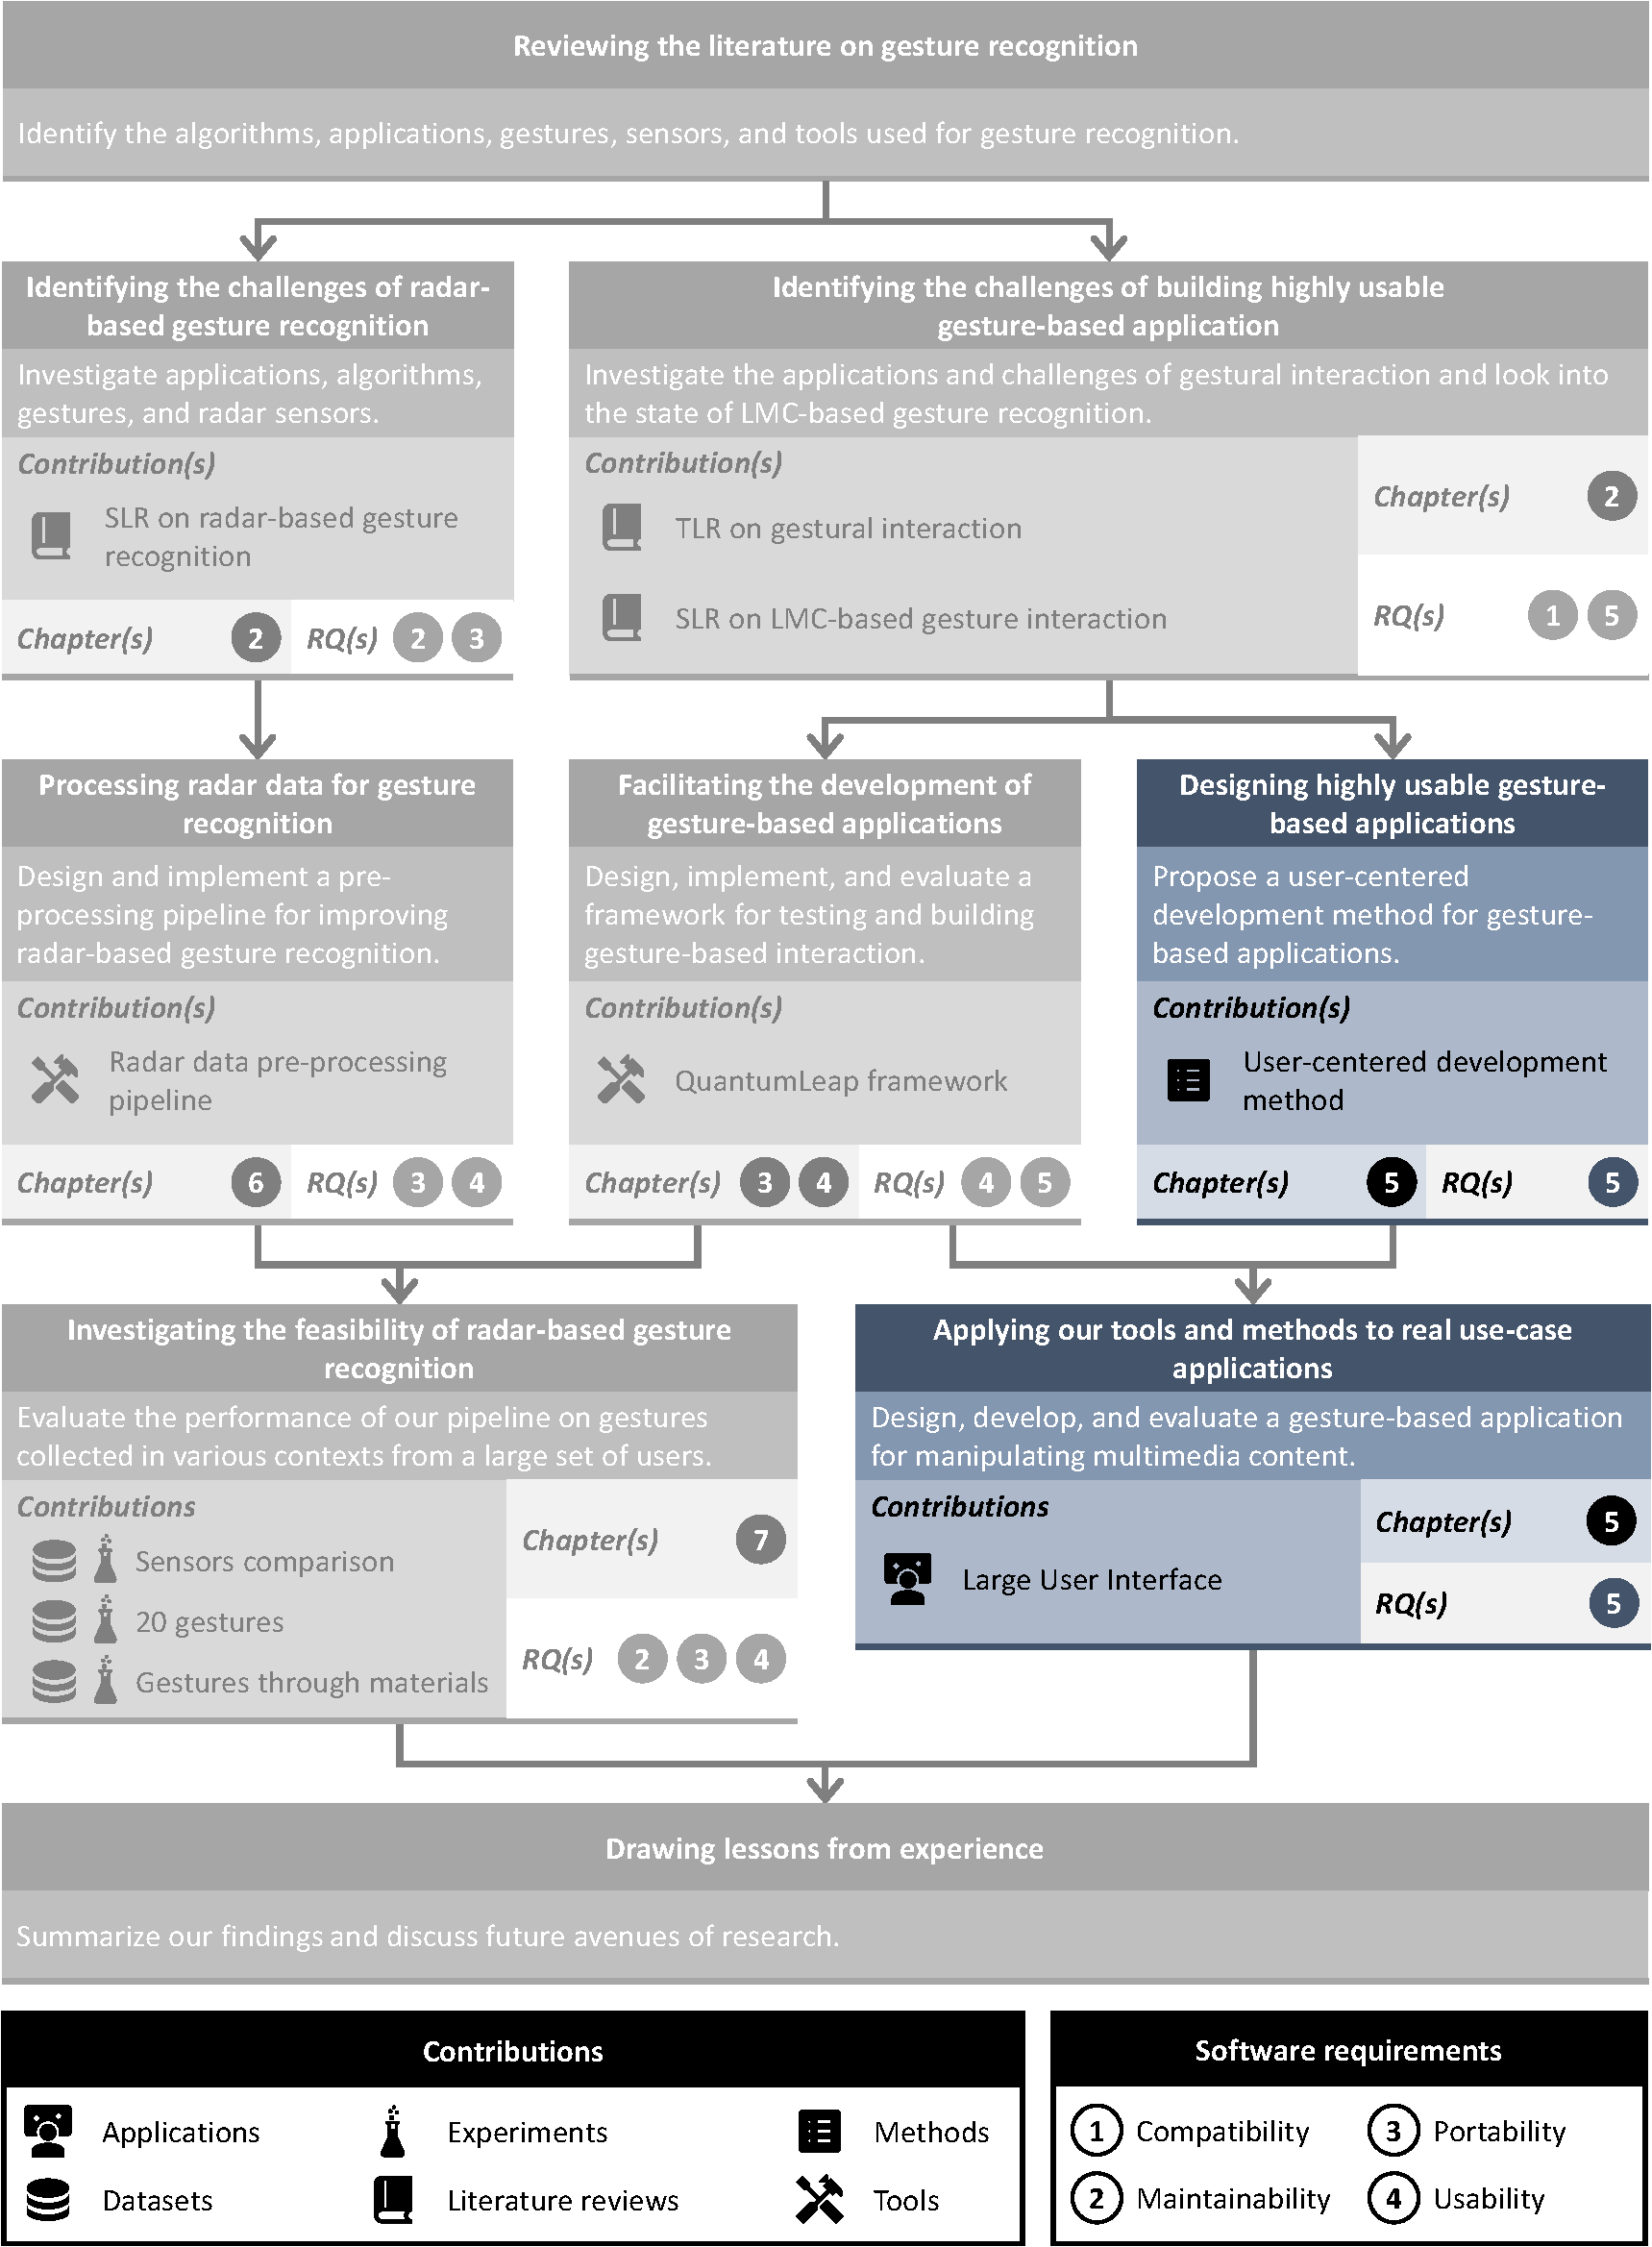
\includegraphics[width=\linewidth]{Figures/LUI/graphical-summary-large-user-interface.pdf}
    \vspace{-18pt}
    \caption{Main contributions of this chapter.}
    \label{fig:lui:graphical-summary}
\end{figure}

The rest of this chapter is organized as follows.
Section~\ref{sec:lui:description} first overviews the \lui application, its concepts, software architecture, and design requirements, and summarizes the differences between its three iterations.
Section~\ref{sec:lui:development-method} then details the stages of the development method used for \lui, including the design of a consistent gesture set, and the use of \ql for testing and implementing gesture interaction.
Section~\ref{sec:lui:evaluation} evaluates the overall quality of the interface, as well as the memorability and efficacy of the implemented gestures.
Finally, Section~\ref{sec:lui:discussion}  discusses the main strengths and limitations of \lui and Section~\ref{sec:lui:conclusion} concludes this chapter.

\paragraph{Publications.} This chapter is based on two papers published in the IJHCI journal~\cite{Sluyters:2022:LUI} and IJHCS journal~\cite{Sellier:2024}.

\paragraph{Resources.} The \lui application source code and its \ql configuration are available on GitHub at \url{https://github.com/sluyters/LUI}. Demonstration videos of \lui are available at \url{https://www.youtube.com/playlist?list=PLj1KcEqIa0fGRb0Z5E7f0UoL4LaxiKbm4}.

%================================================================================%
\section{The \lui Application} \label{sec:lui:description}

%--------------------------------------------------------------------------------%
\subsection{Overview} \label{sec:lui:description:overview}
\lui is a gesture-based interactive application for manipulating multimedia objects on large displays, such as TVs and wall displays, in a semi-public environment.
It currently focuses on interaction with photos, videos, documents, and maps, for which different sets of functions are desired (\tab~\ref{tab:lui:media-actions}). \lui is designed to be widely distributed and easily installed by being cheap to set up and easy to use. As such, we settled on using the Leap Motion Controller (LMC)\footnote{See \url{https://www.ultraleap.com/product/leap-motion-controller/}} for hand tracking, a cheap off-the-shelf sensor (less than 100\$) that can be plugged via USB to the computer. We selected the LMC for mid-air gesture interaction because it tracks two hands and their ten fingers~\cite{Colgan:2017} with high precision and robustness~\cite{Weichert:2013}, including the palm vector and hand radius. This sensor is comprised of two cameras and three infrared (IR) LEDs. The interaction space is .6m wide by .6m long by .6m deep, resulting in an .22 cubic meter volumetric space which takes the shape of an inverted pyramid above the sensor.
The LMC API~\cite{Spiegelmock:2013} enables to natively recognize a handful of system-defined gestures~\cite{Brandon:2014}, but custom gesture recognition algorithms often support a wider range of gestures~\cite{Bachmann:2018}. The LMC benefits from better accuracy and precision than other devices, such as an MS Kinect~\cite{Guzsvinecz:2019} or an Intel RealSense~\cite{Khalaf:2019}.
It is also widely used in many domains of applications such as augmented reality~\cite{Lopez:2015} and activity recognition~\cite{Marin:2016}. Several LMC-based gesture recognition algorithms exist~\cite{Bachmann:2018}. No study compares them on the same basis, apart from \cite{Filho:2018} with three classical machine learning algorithms, but without any recent recognizer such as DeepGru~\cite{Maghoumi:2019}.

\begin{table}
%    \vspace{-11pt}
    \footnotesize
    \centering
    \begin{tabular}{lcccc}
        \toprule
        \multicolumn{1}{c}{\multirow{2}{*}{\textbf{Function}}} & \multicolumn{4}{c}{\textbf{Media type}} \\
        & Photos & Videos & Documents & Maps \\
        \midrule
        Fullscreen on/off & \fullcirc & \fullcirc & \fullcirc & \fullcirc \\
        Like/dislike & \fullcirc & \fullcirc & \fullcirc & \fullcirc \\
        Previous/Next & \fullcirc & \fullcirc & \fullcirc & \emptycirc \\
        Zoom in/out & \fullcirc & \emptycirc & \fullcirc & \fullcirc \\
        Rotate & \fullcirc & \emptycirc & \fullcirc & \fullcirc \\
        Pan & \fullcirc & \emptycirc & \fullcirc & \fullcirc \\
        Change brightness & \fullcirc & \emptycirc & \emptycirc & \emptycirc \\
        Change contrast & \fullcirc & \emptycirc & \emptycirc & \emptycirc \\
        Play/pause & \emptycirc & \fullcirc & \emptycirc & \emptycirc \\
        Show/hide subtitles & \emptycirc & \fullcirc & \emptycirc & \emptycirc \\
        Volume up/down & \emptycirc & \fullcirc & \emptycirc & \emptycirc \\
        Fast-forward/backward & \emptycirc & \fullcirc & \emptycirc & \emptycirc \\
        Highlight text & \emptycirc & \emptycirc & \fullcirc & \emptycirc \\
        Place marker & \emptycirc & \emptycirc & \emptycirc & \fullcirc \\
        Change layer & \emptycirc & \emptycirc & \emptycirc & \fullcirc \\
        \bottomrule
    \end{tabular}
    \vspace{-4pt}
    \caption{List of functions for each media type.}
    % \vspace{-10pt}
    \label{tab:lui:media-actions}
\end{table}

\begin{figure}[p]
    \centering
    % \vspace{-10pt}
    \begin{subfigure}{.47\textwidth}
        \centering
        
\includegraphics[width=.96\linewidth]{Figures/LUI/UI/welcome_screen_lui.pdf}  
        \vspace{-5pt}
        \captionsetup{width=.9\linewidth}
        \caption{Welcome screen.}
        \label{fig:lui:screenshots:welcome-screen}
    \end{subfigure}
    \begin{subfigure}{.47\textwidth}
        \centering
        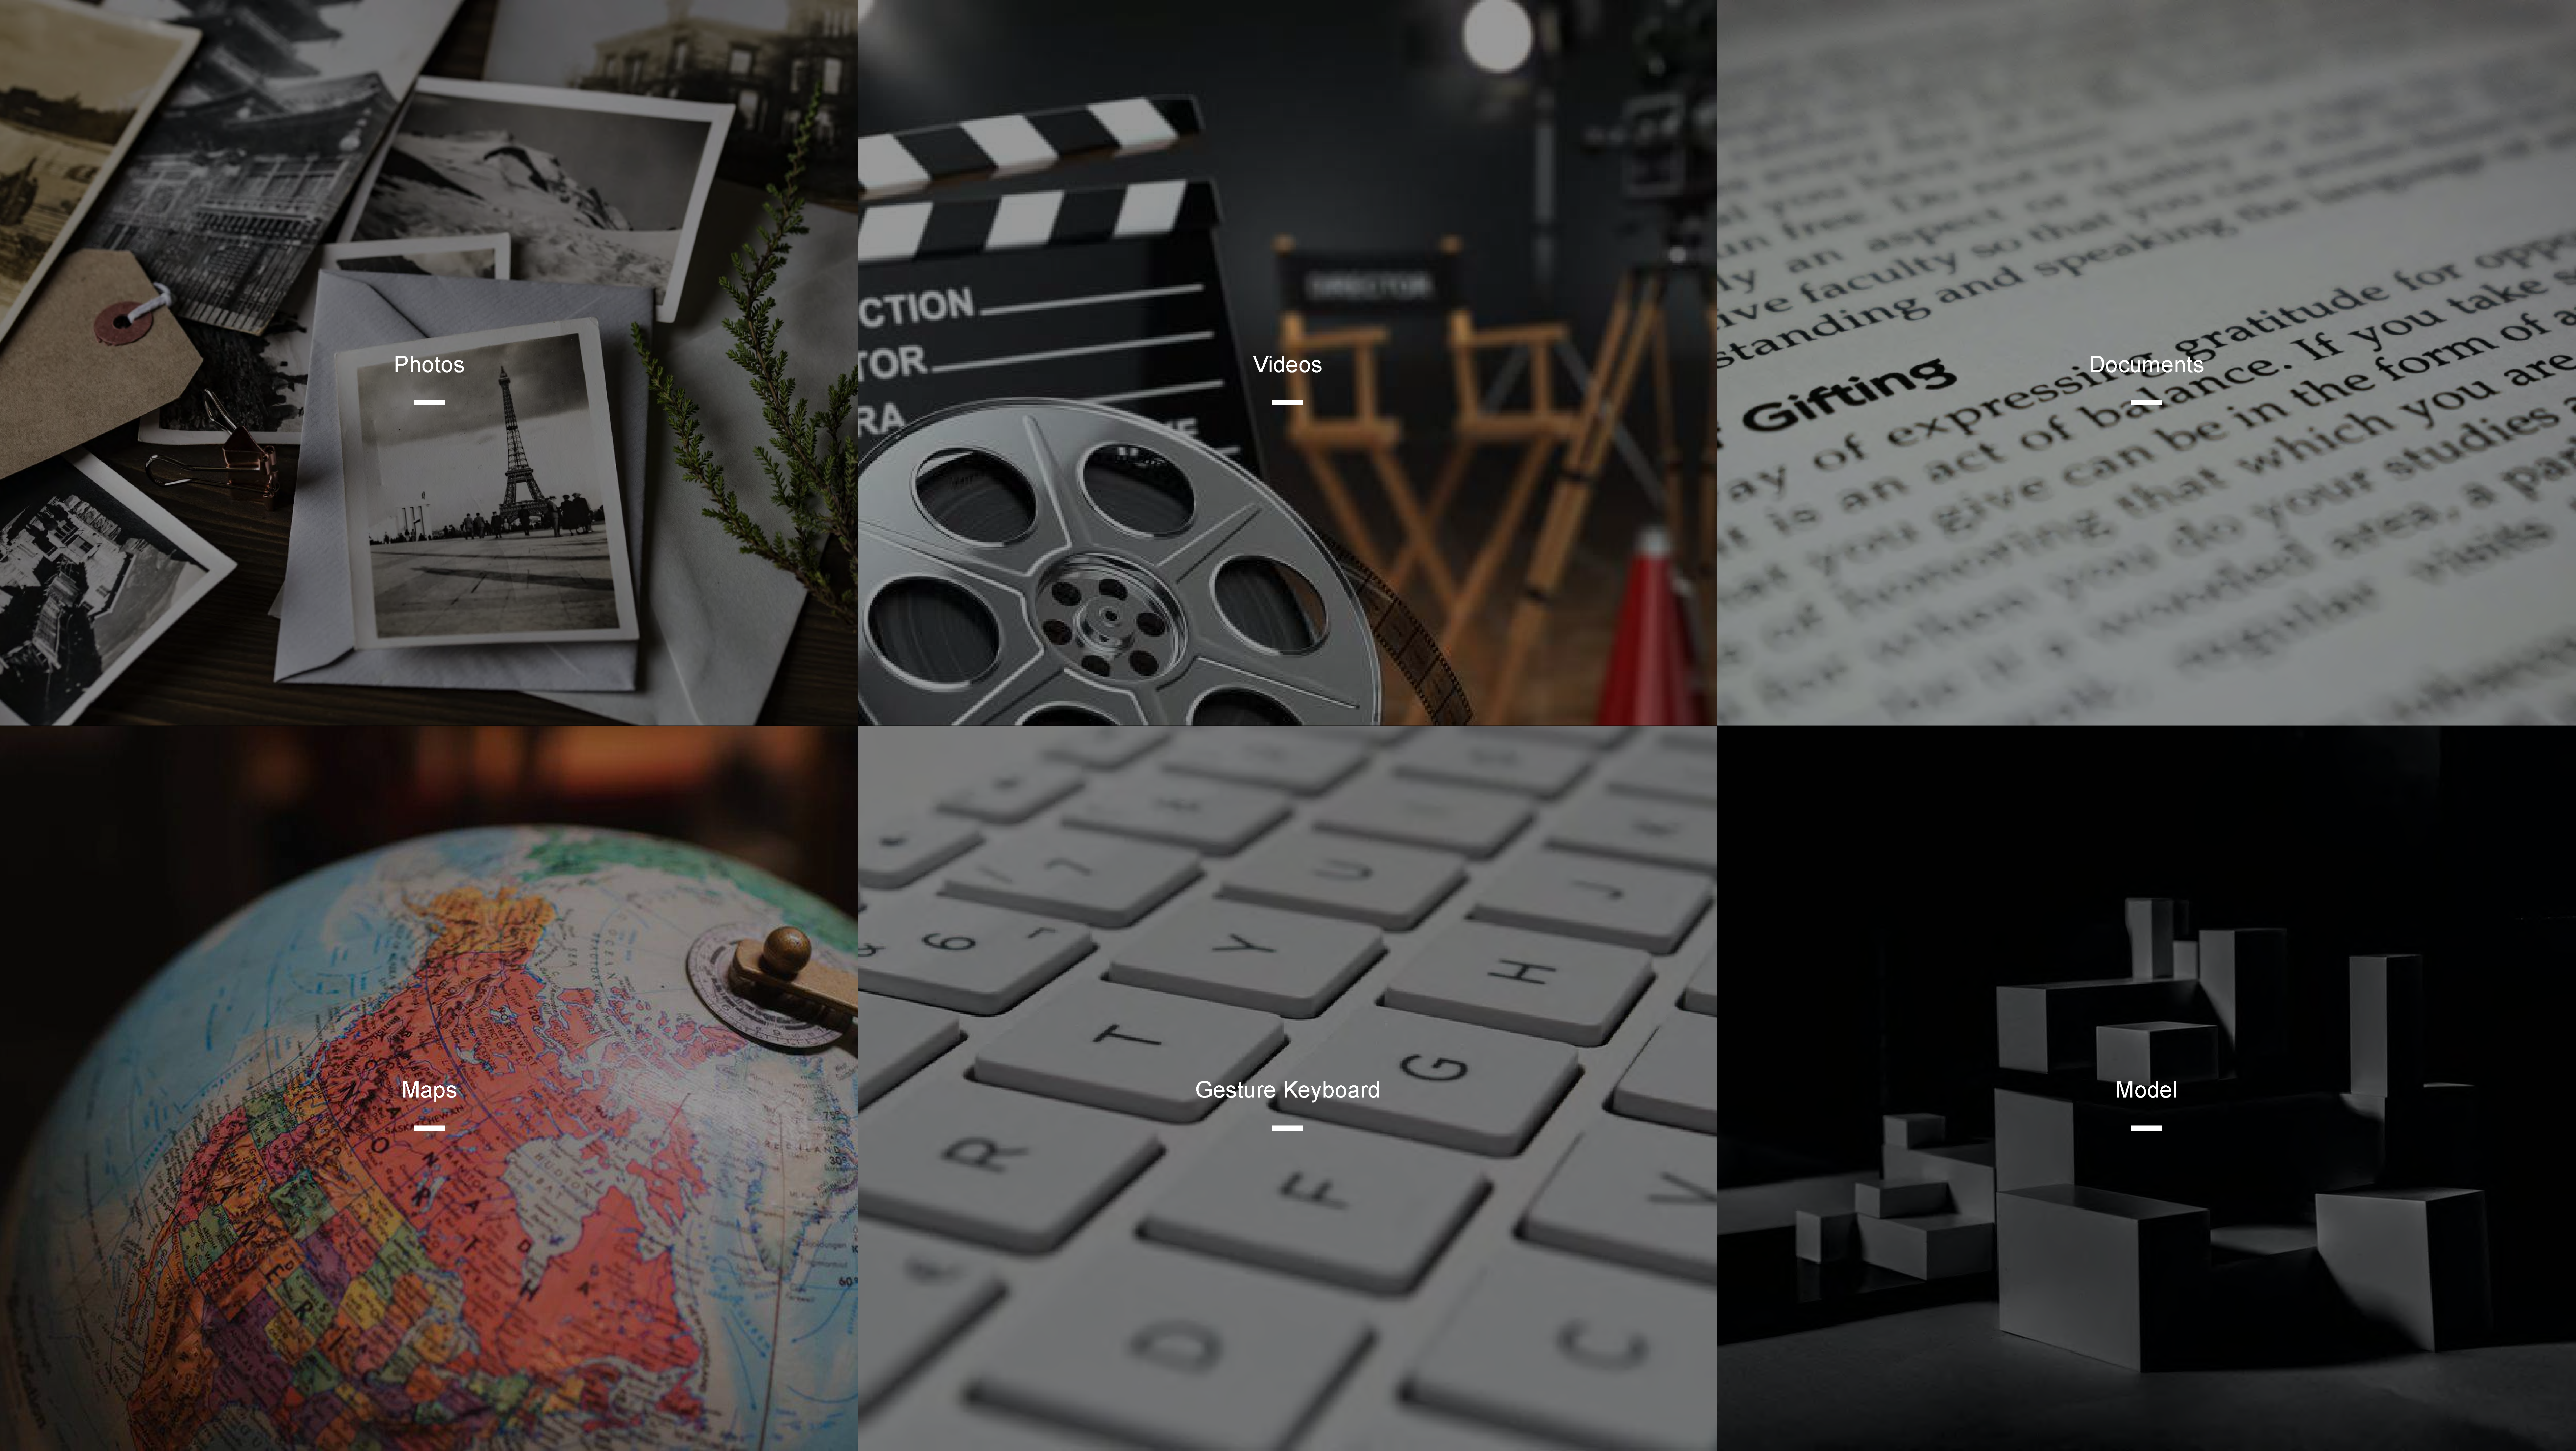
\includegraphics[width=.96\linewidth]{Figures/LUI/UI/app_menu.pdf}  
        \vspace{-5pt}
        \captionsetup{width=.9\linewidth}
        \caption{Application menu.}
        \label{fig:lui:screenshots:app-menu}
    \end{subfigure}

    \begin{subfigure}{.47\textwidth}
        \centering
        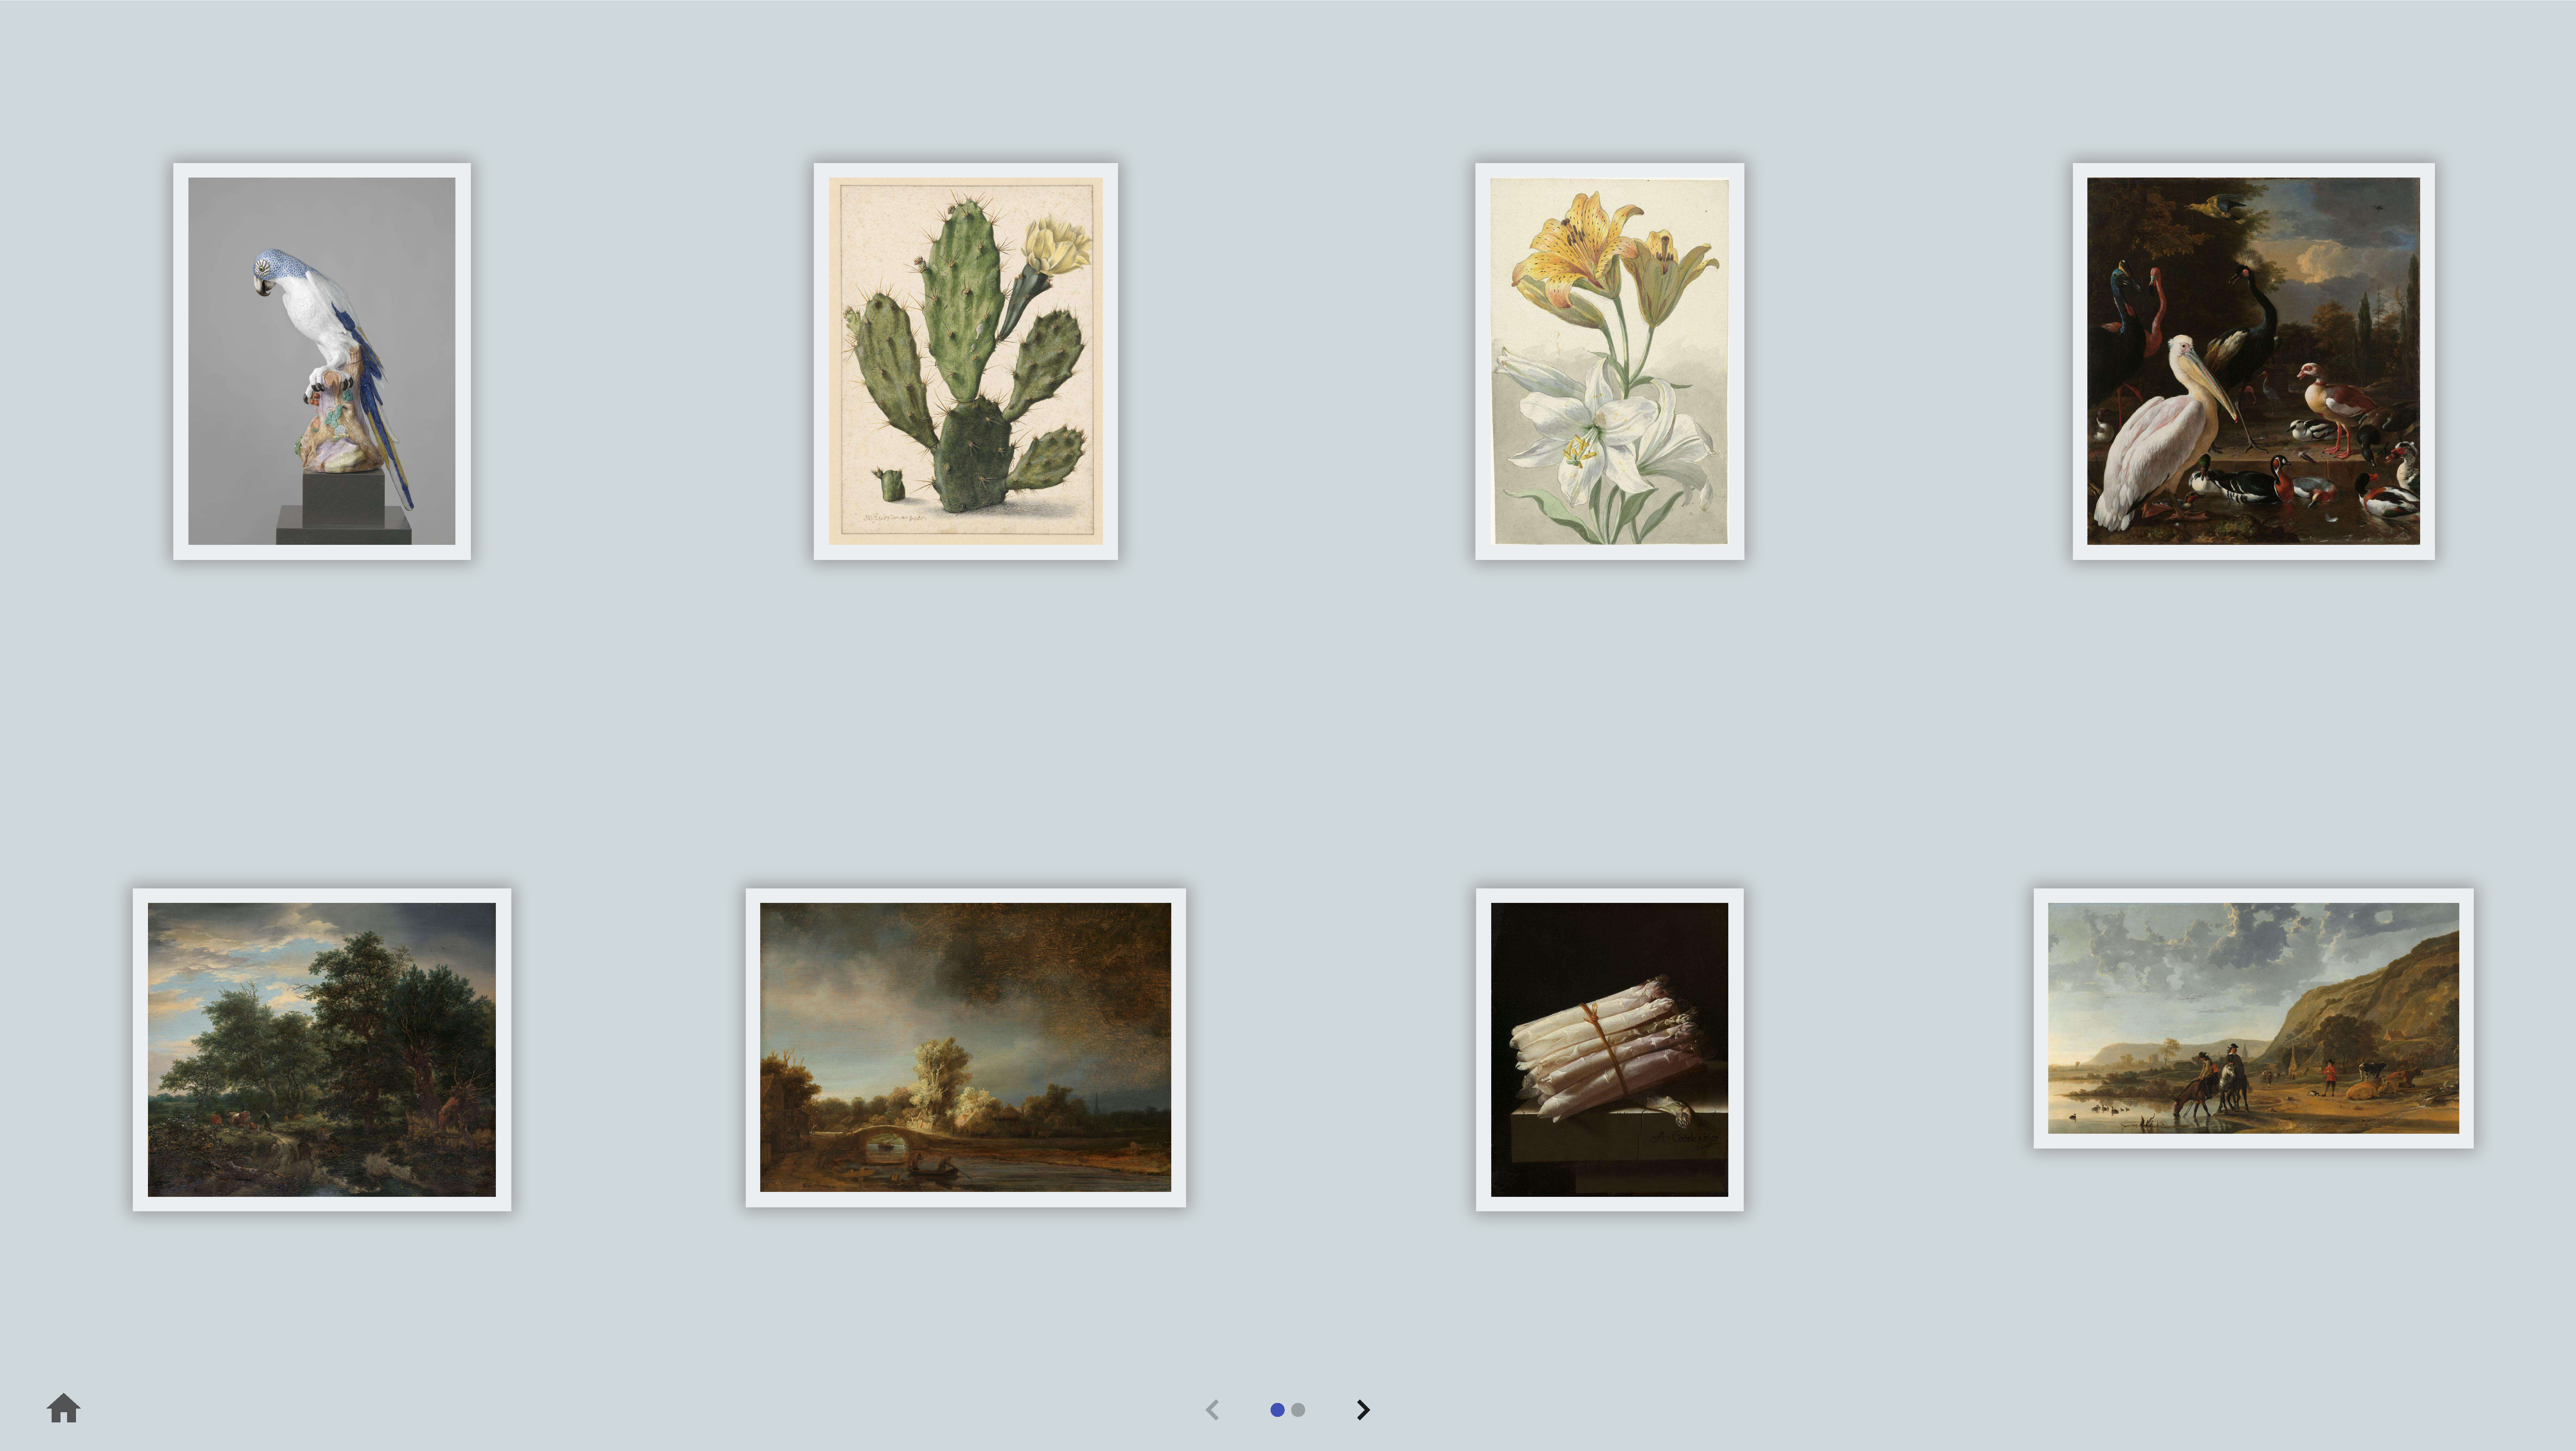
\includegraphics[width=.96\linewidth]{Figures/LUI/UI/photos-list.pdf}  
        \vspace{-5pt}
        \captionsetup{width=.9\linewidth}
        \caption{Photos app (list).}
        \label{fig:lui:screenshots:photos-list}
    \end{subfigure}
    \begin{subfigure}{.47\textwidth}
        \centering
        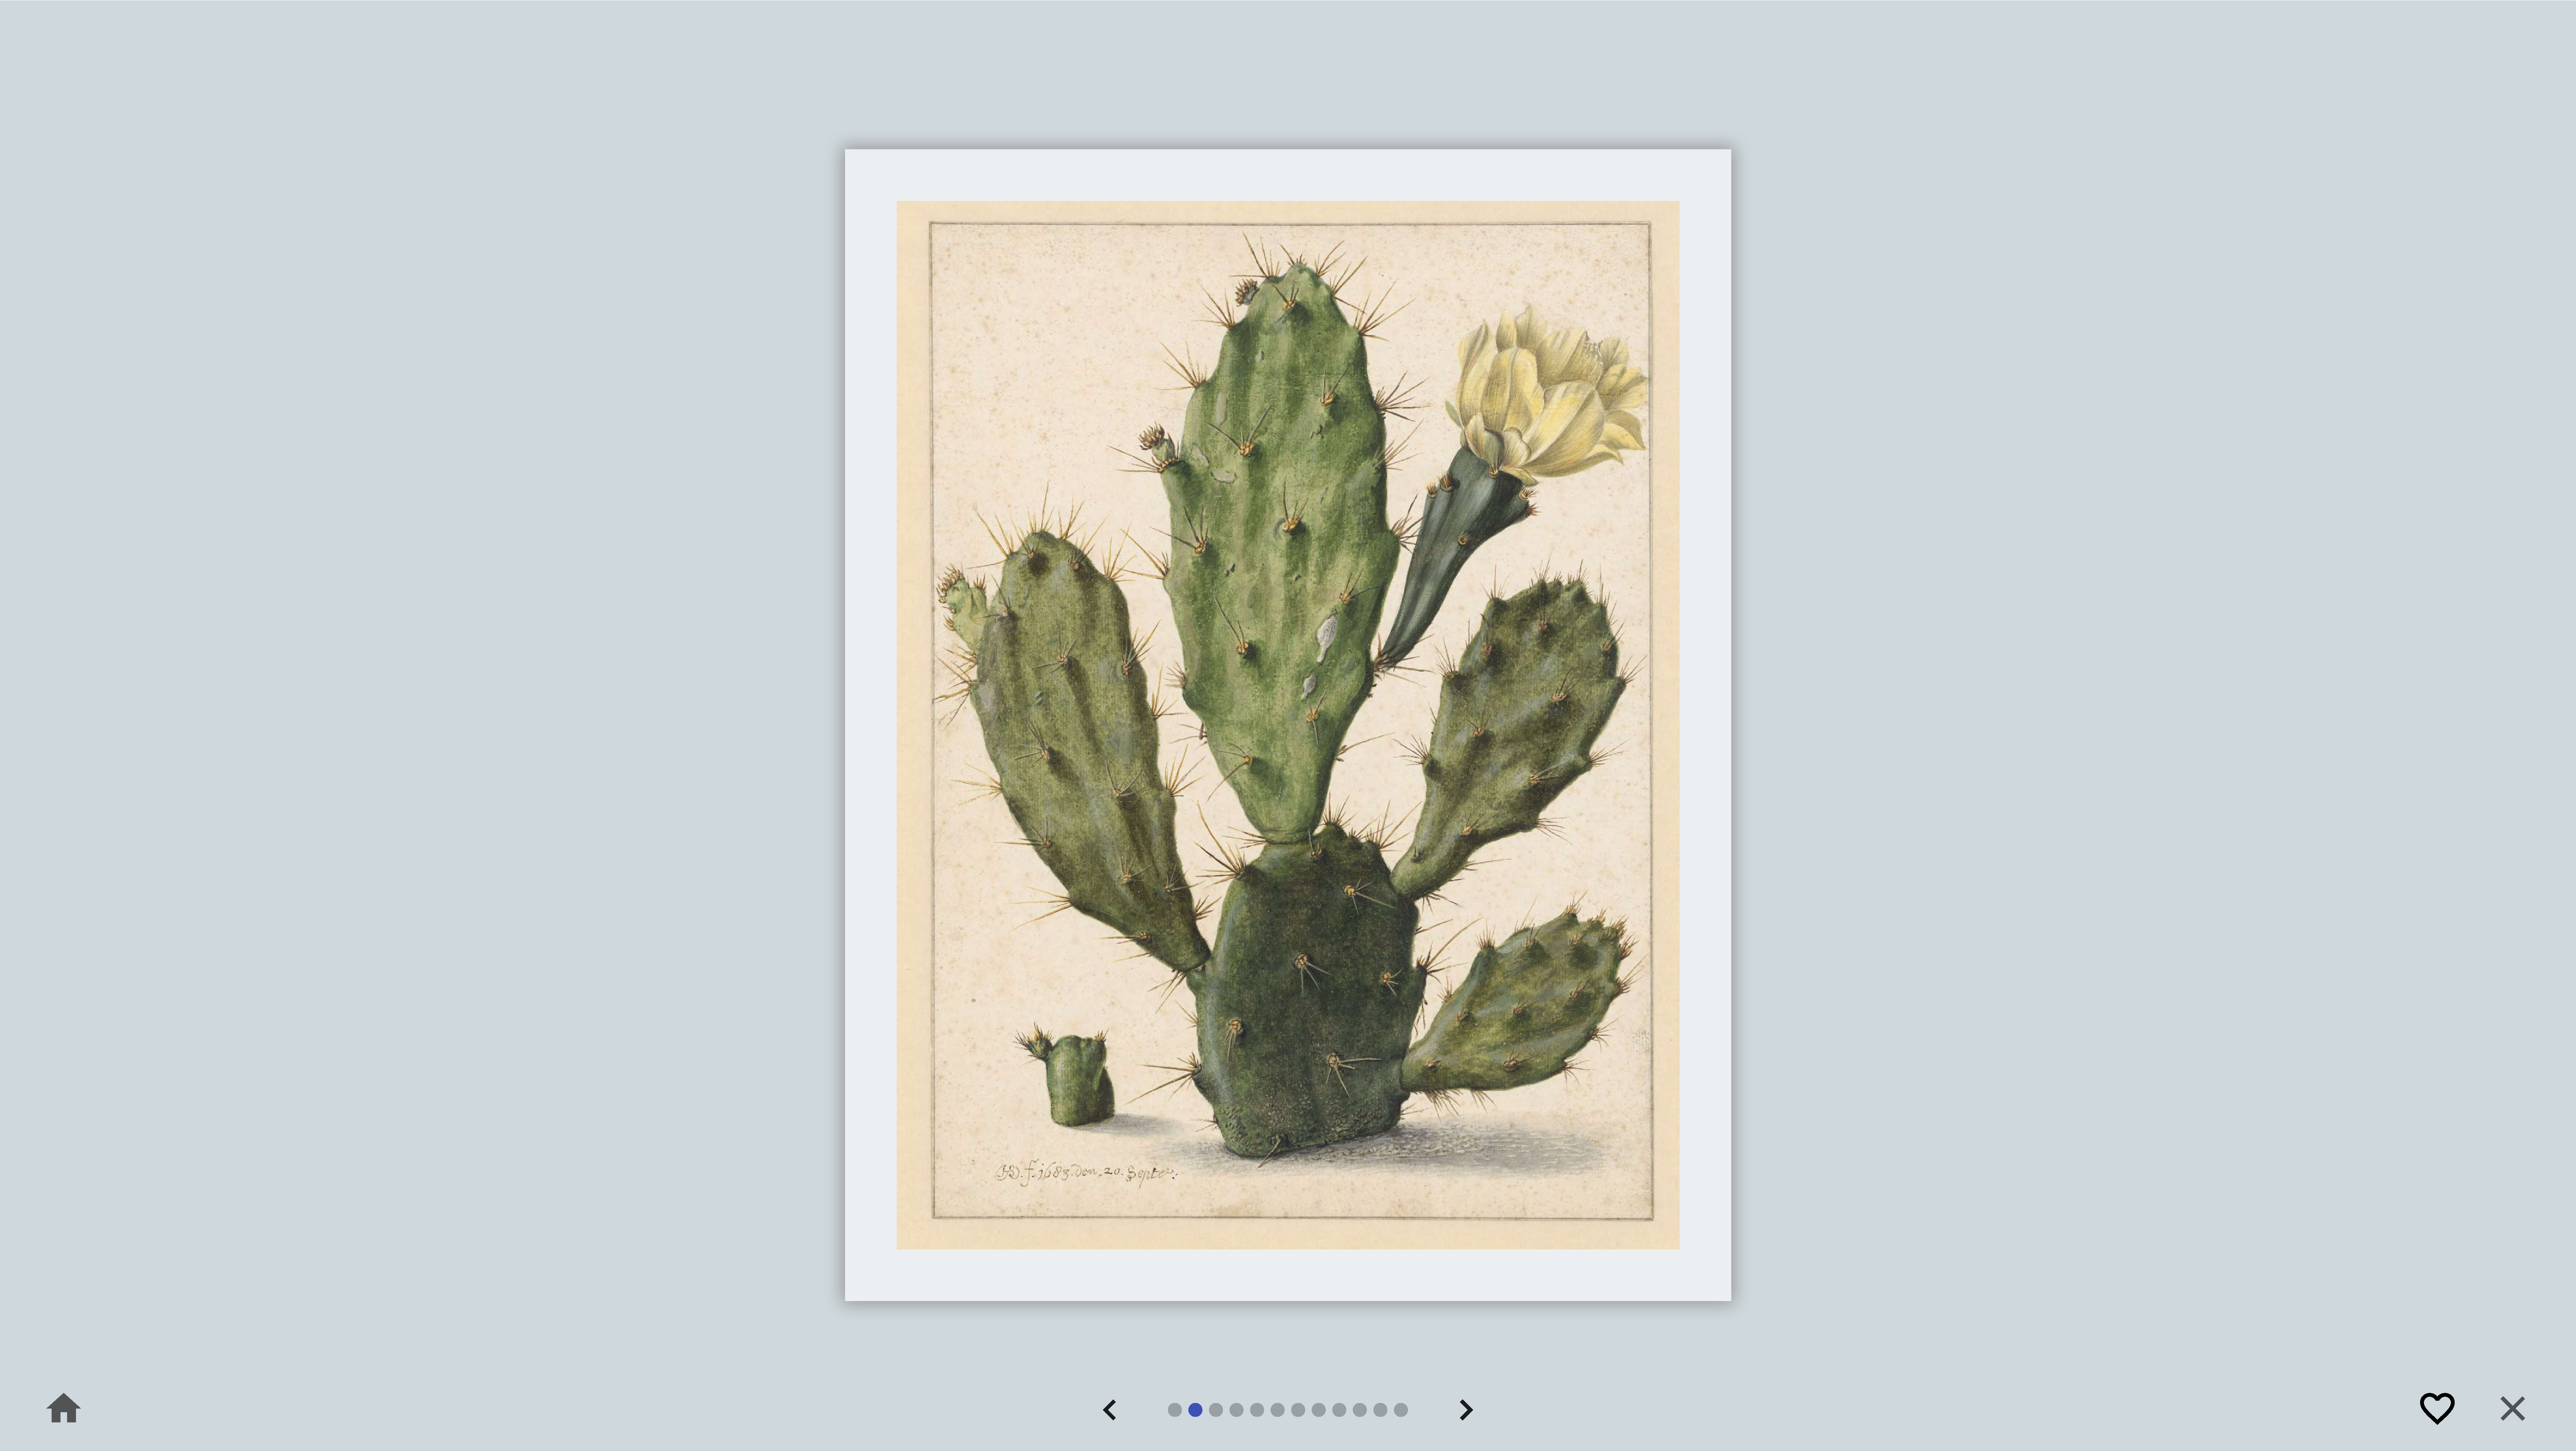
\includegraphics[width=.96\linewidth]{Figures/LUI/UI/photos-fullscreen.pdf}  
        \vspace{-5pt}
        \captionsetup{width=.9\linewidth}
        \caption{Photos app (item).}
        \label{fig:lui:screenshots:photos-fullscreen}
    \end{subfigure}

    \begin{subfigure}{.47\textwidth}
        \centering
        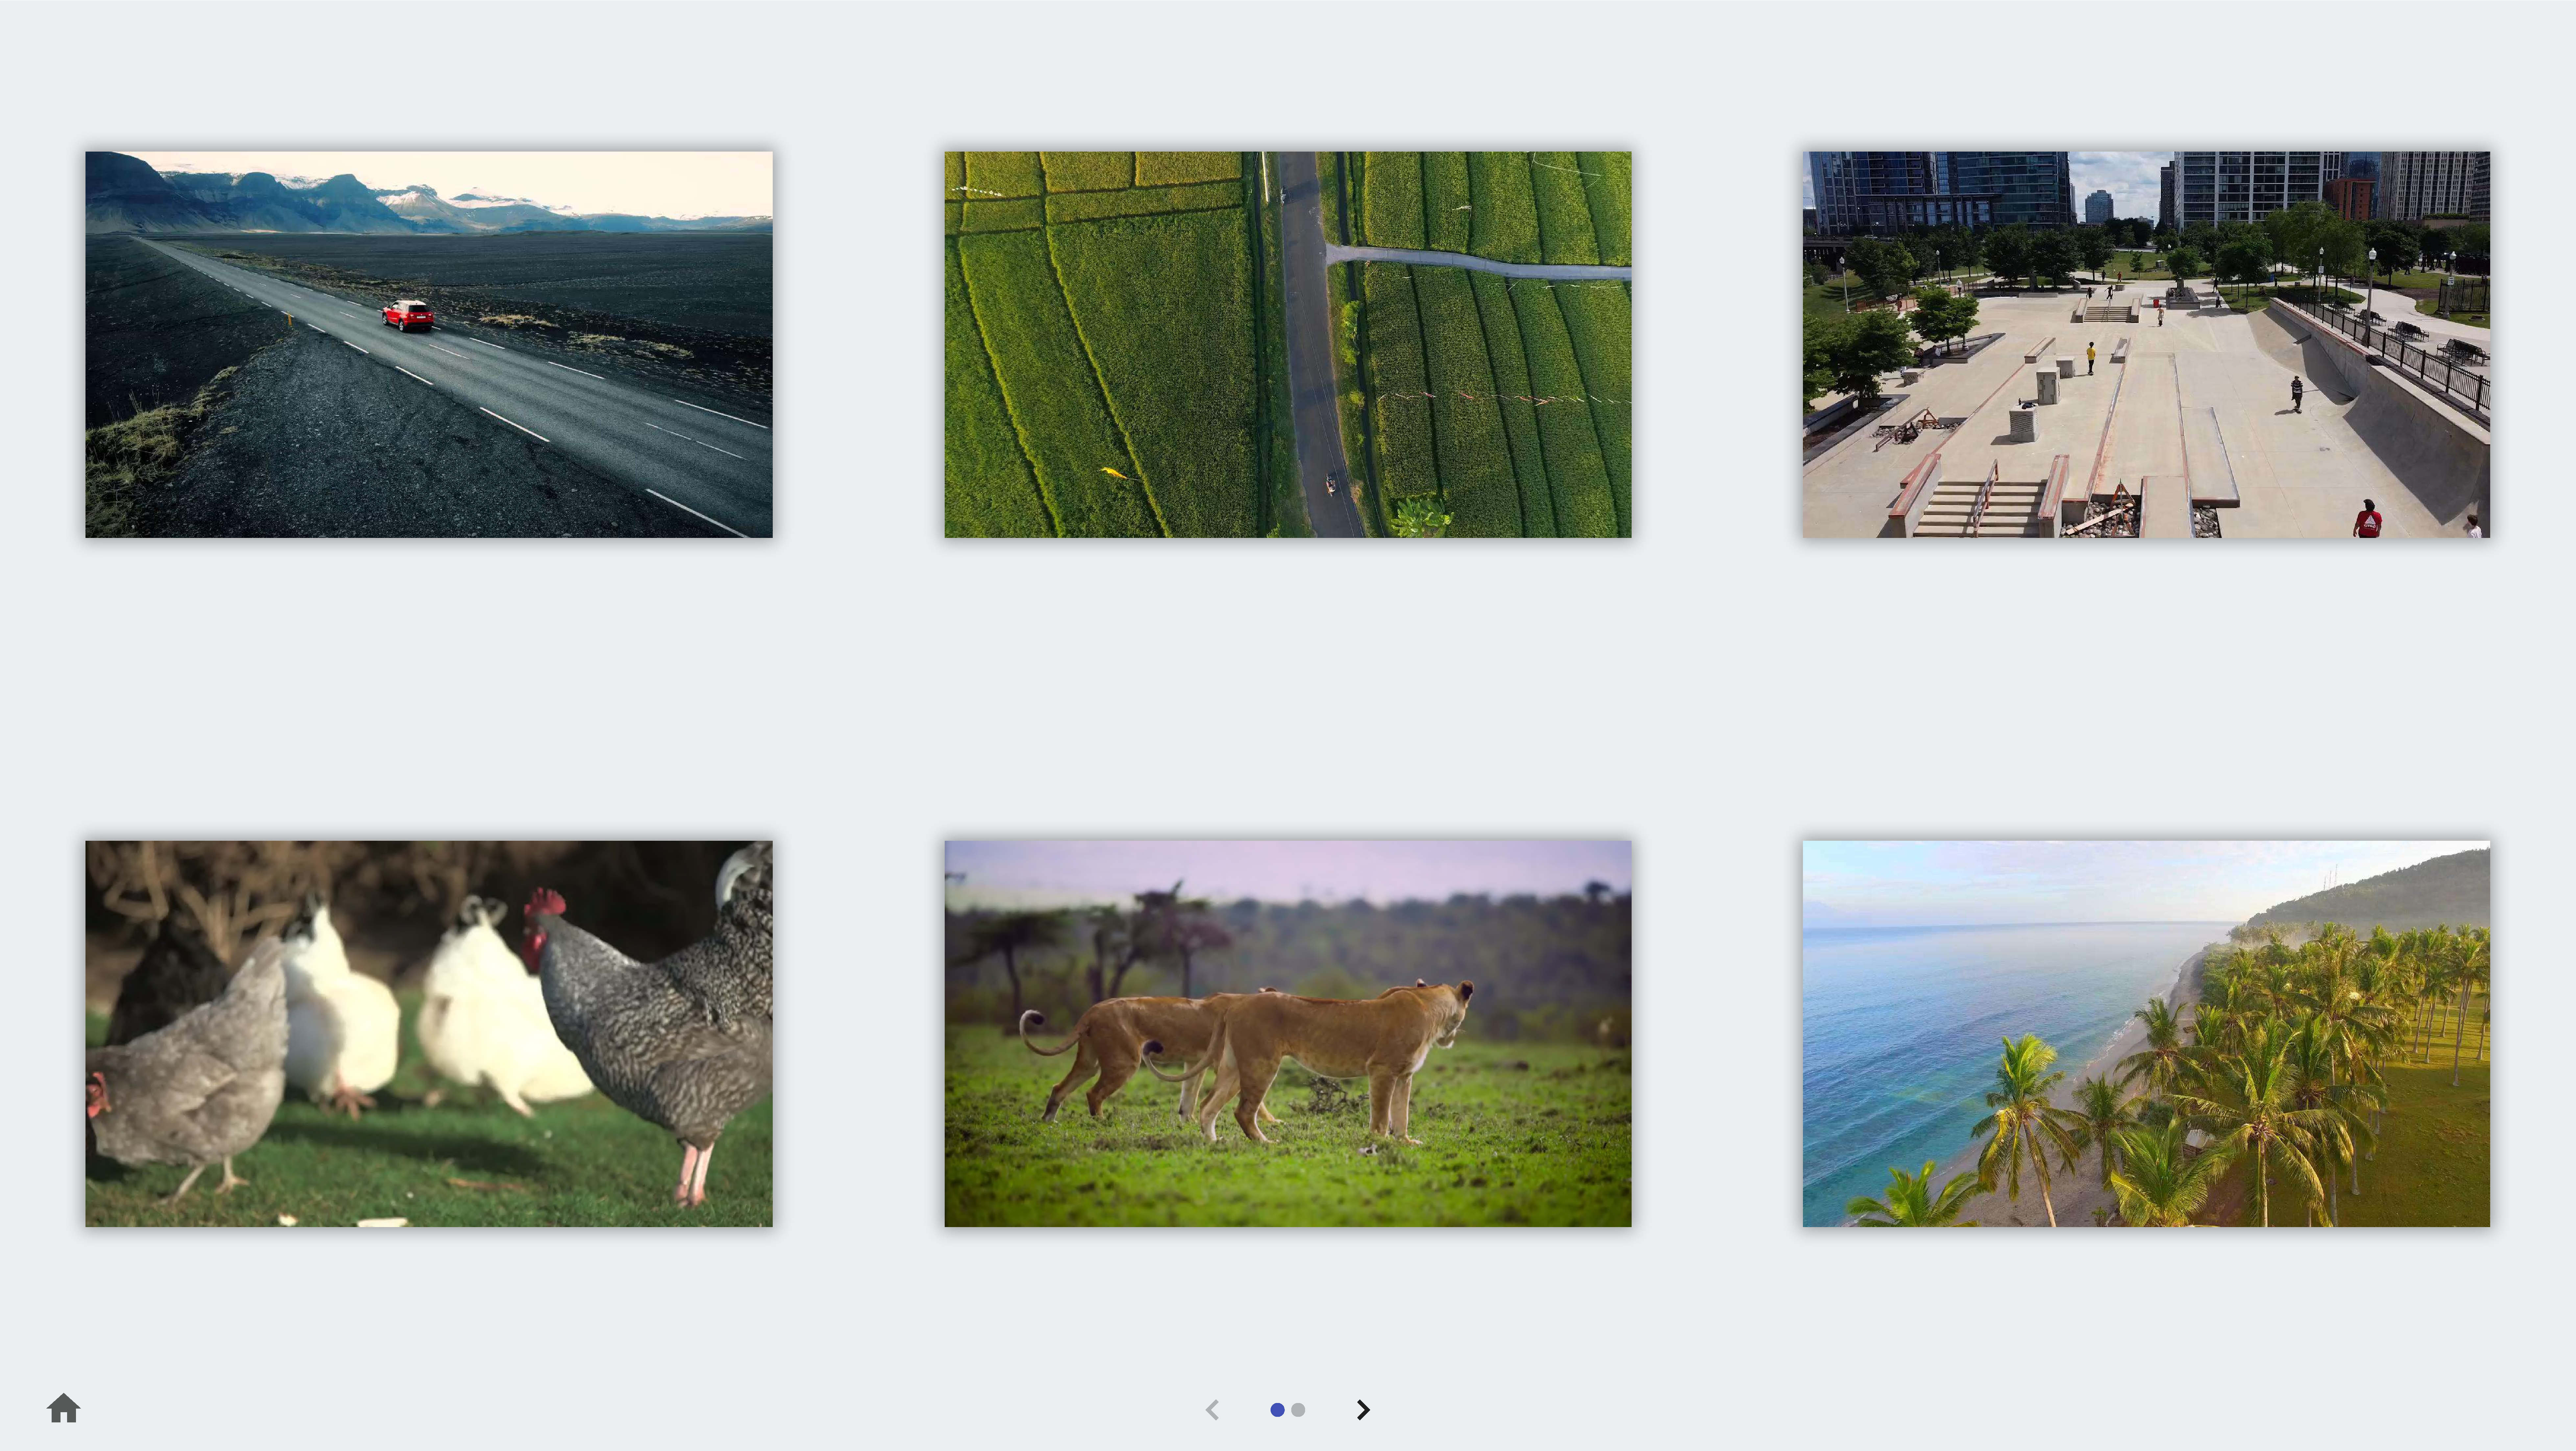
\includegraphics[width=.96\linewidth]{Figures/LUI/UI/videos-list.pdf} 
        \vspace{-5pt}
        \captionsetup{width=.9\linewidth}
        \caption{Videos app (list).}
        \label{fig:lui:screenshots:videos-list}
    \end{subfigure}
    \begin{subfigure}{.47\textwidth}
        \centering
        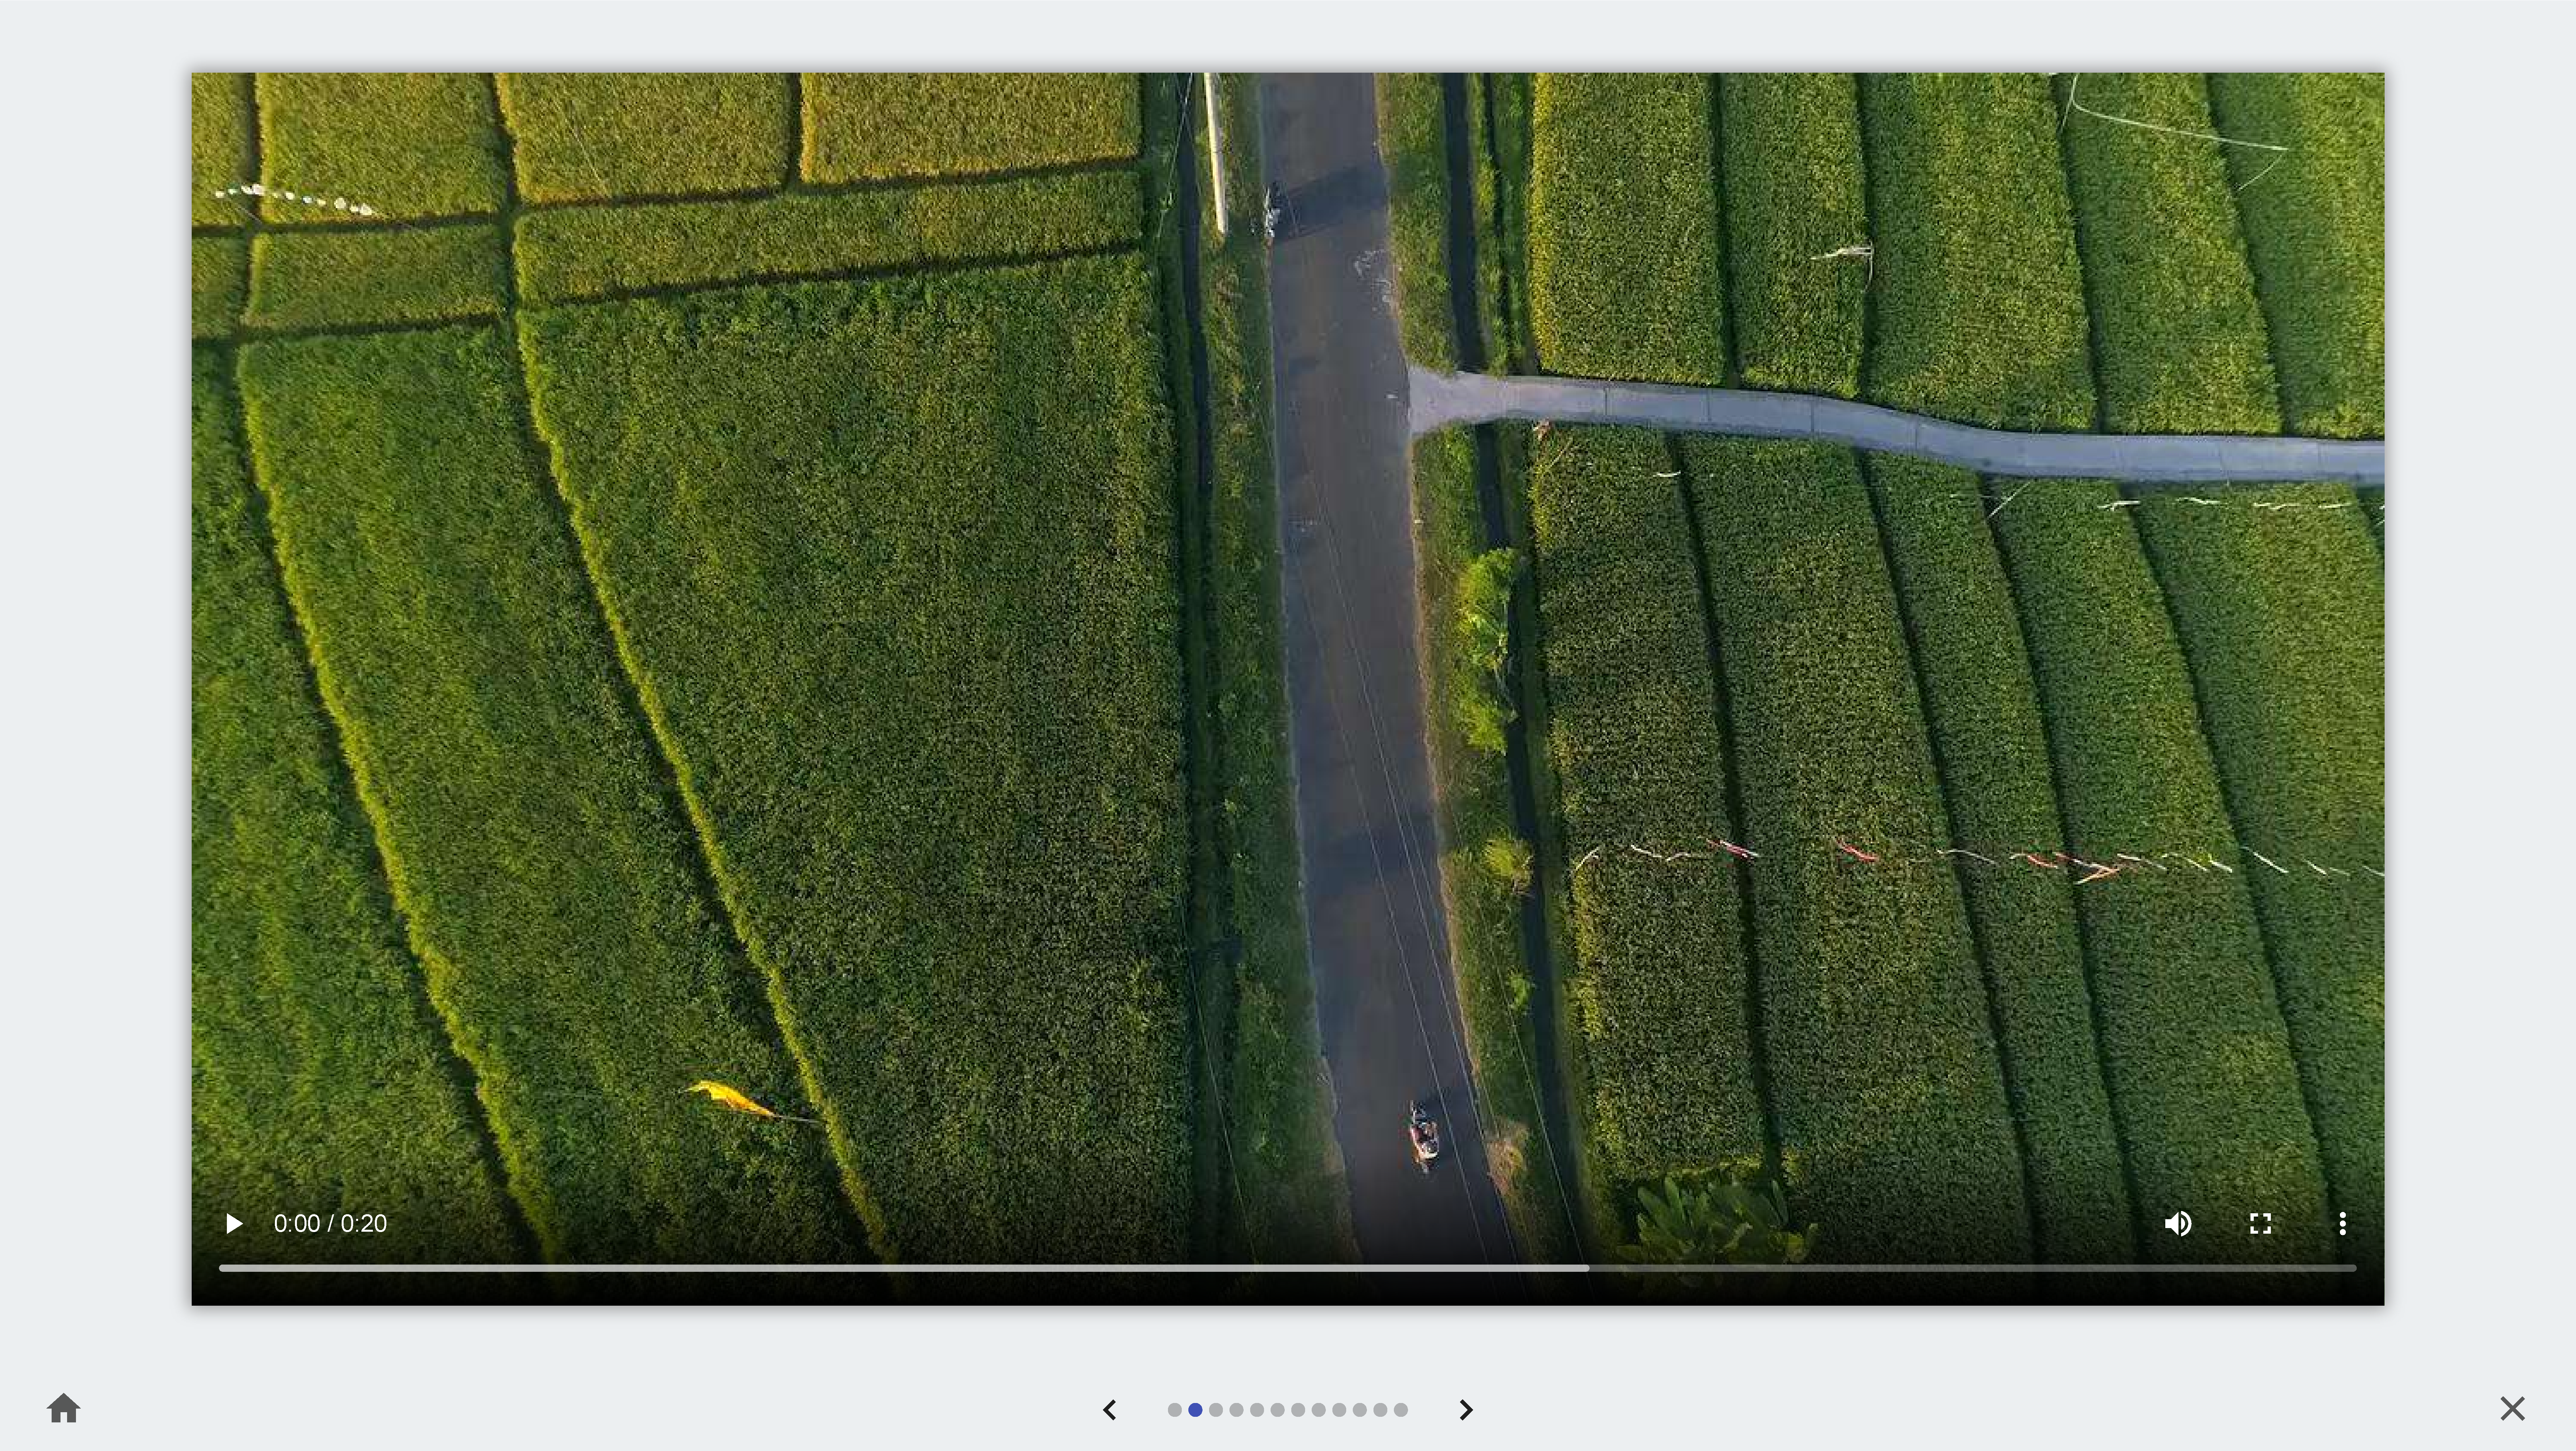
\includegraphics[width=.96\linewidth]{Figures/LUI/UI/videos-fullscreen.pdf}  
        \vspace{-5pt}
        \captionsetup{width=.9\linewidth}
        \caption{Videos app (item).}
        \label{fig:lui:screenshots:videos-fullscreen}
    \end{subfigure}

    \begin{subfigure}{.47\textwidth}
        \centering
        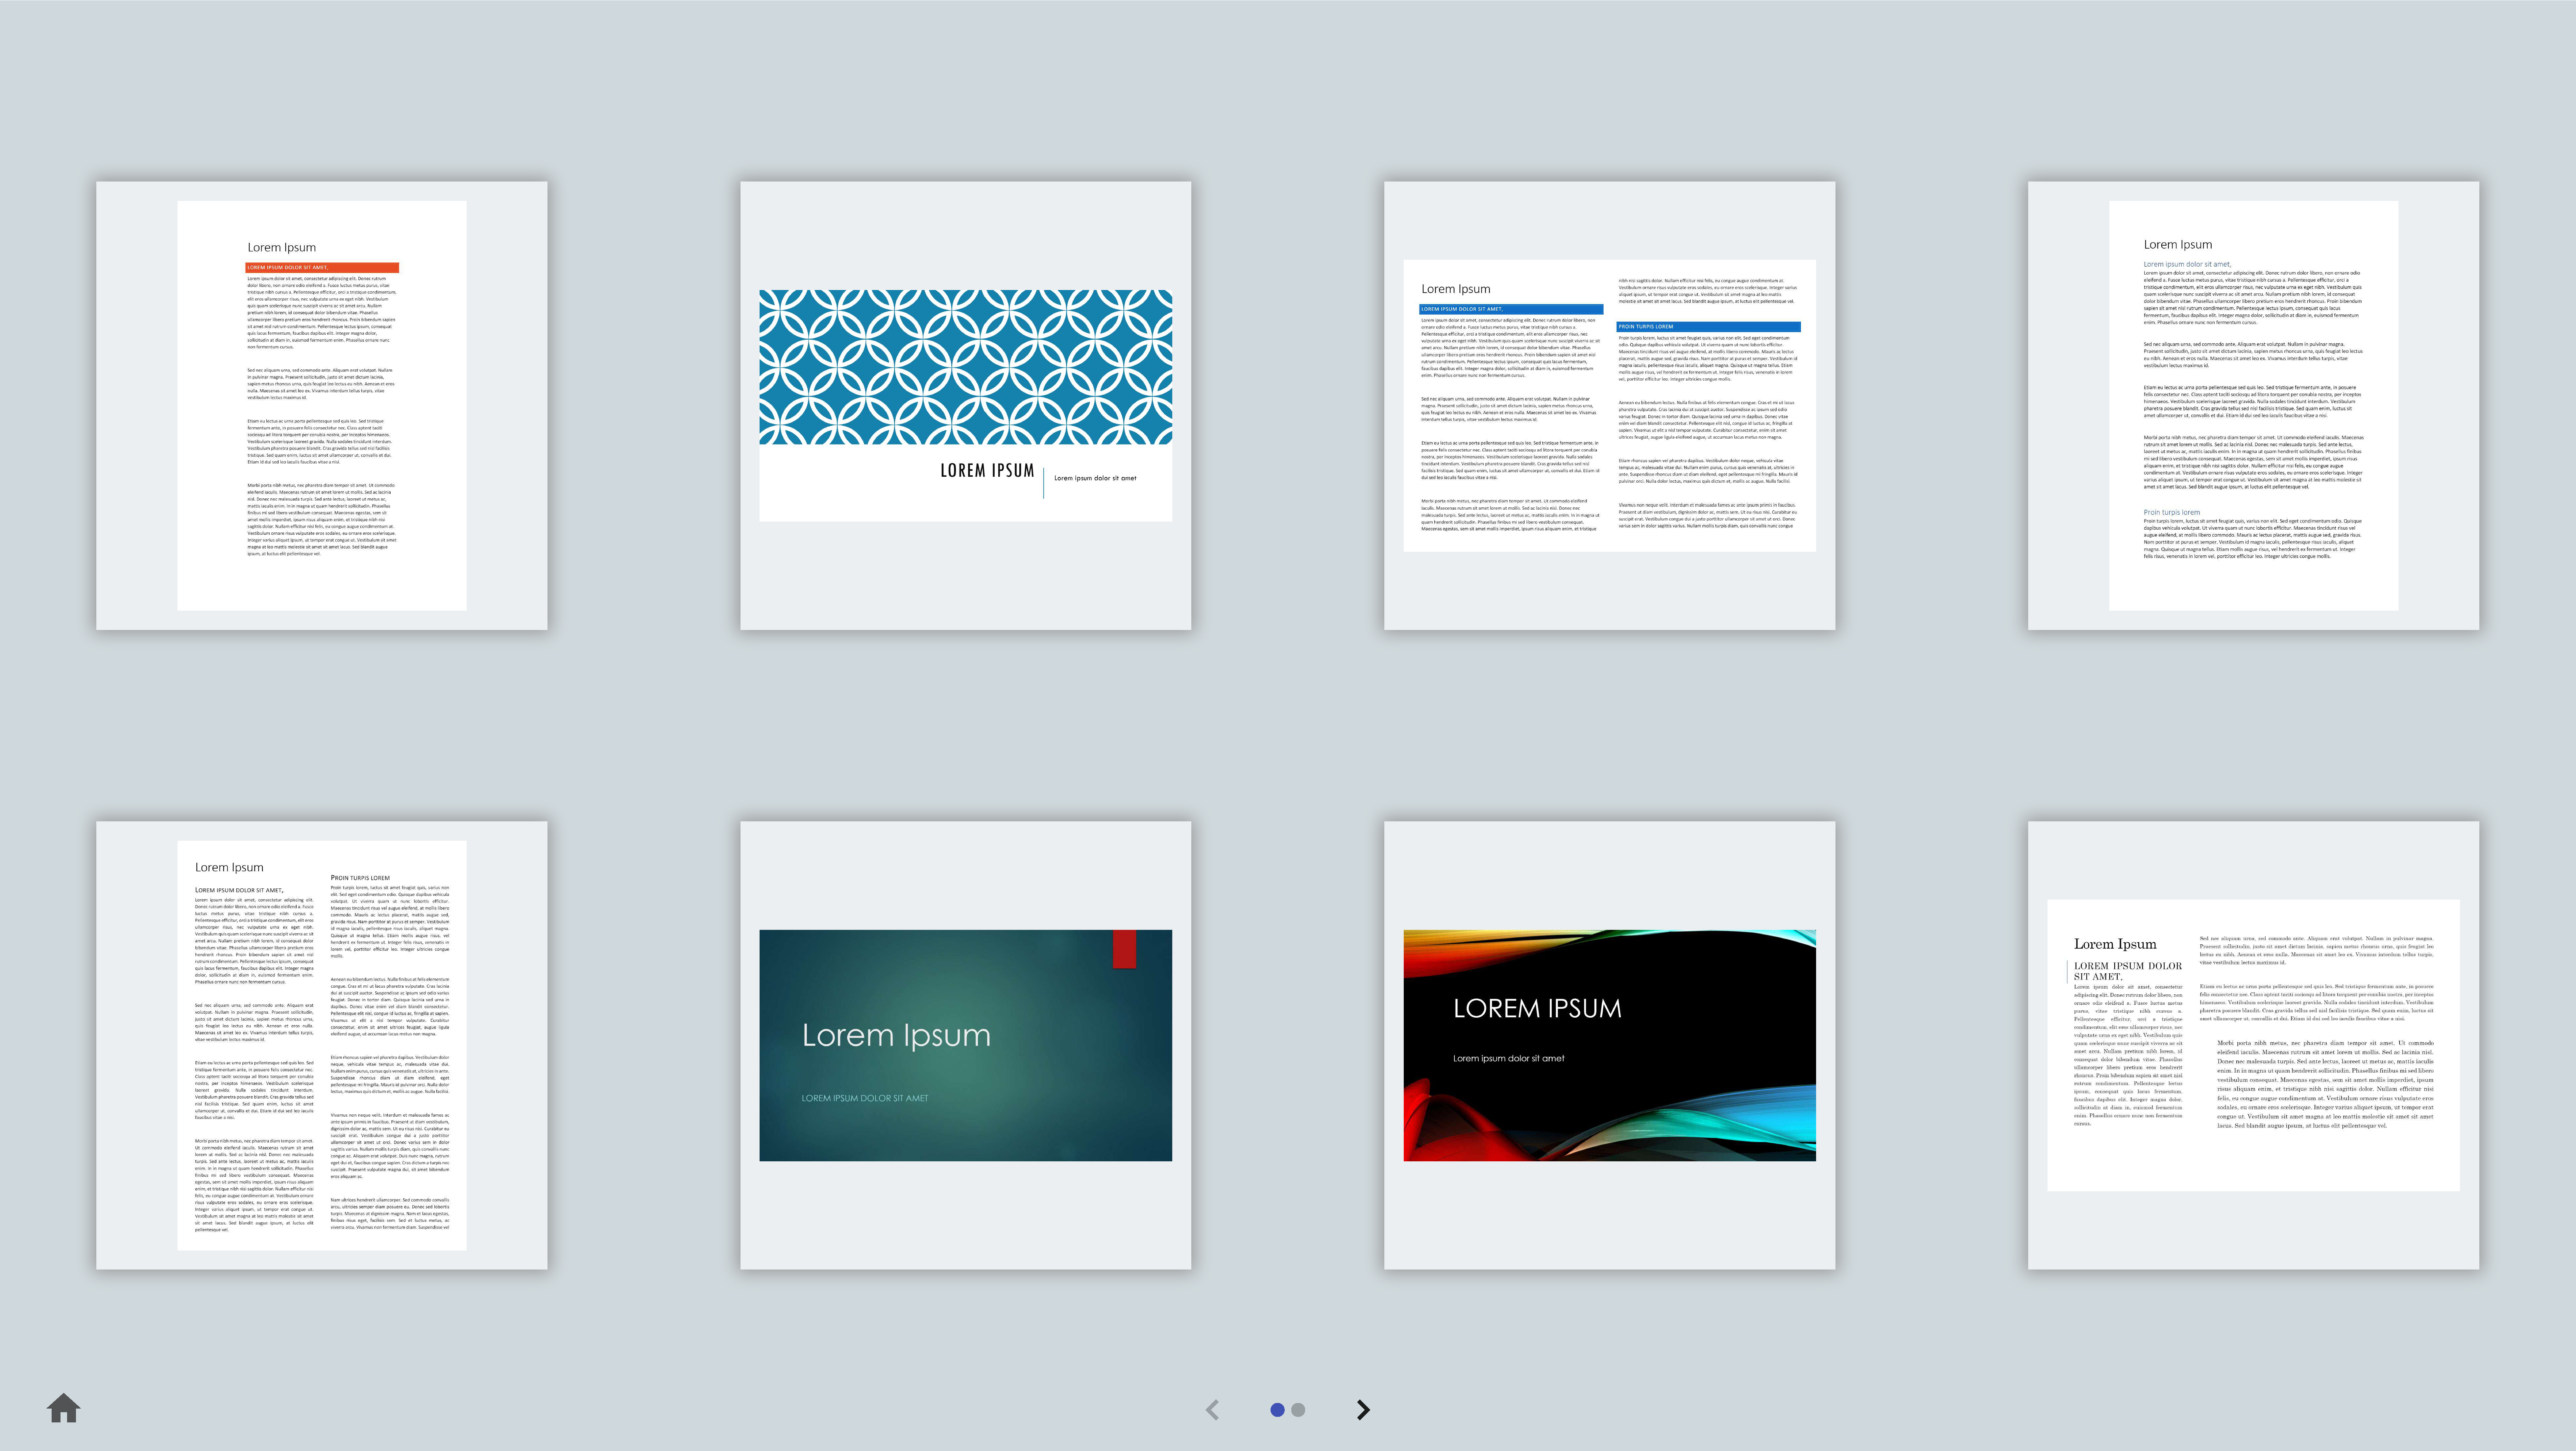
\includegraphics[width=.96\linewidth]{Figures/LUI/UI/documents-list.pdf} 
        \vspace{-5pt}
        \captionsetup{width=.9\linewidth}
        \caption{Documents app (list).}
        \label{fig:lui:screenshots:documents-list}
    \end{subfigure}
    \begin{subfigure}{.47\textwidth}
        \centering
        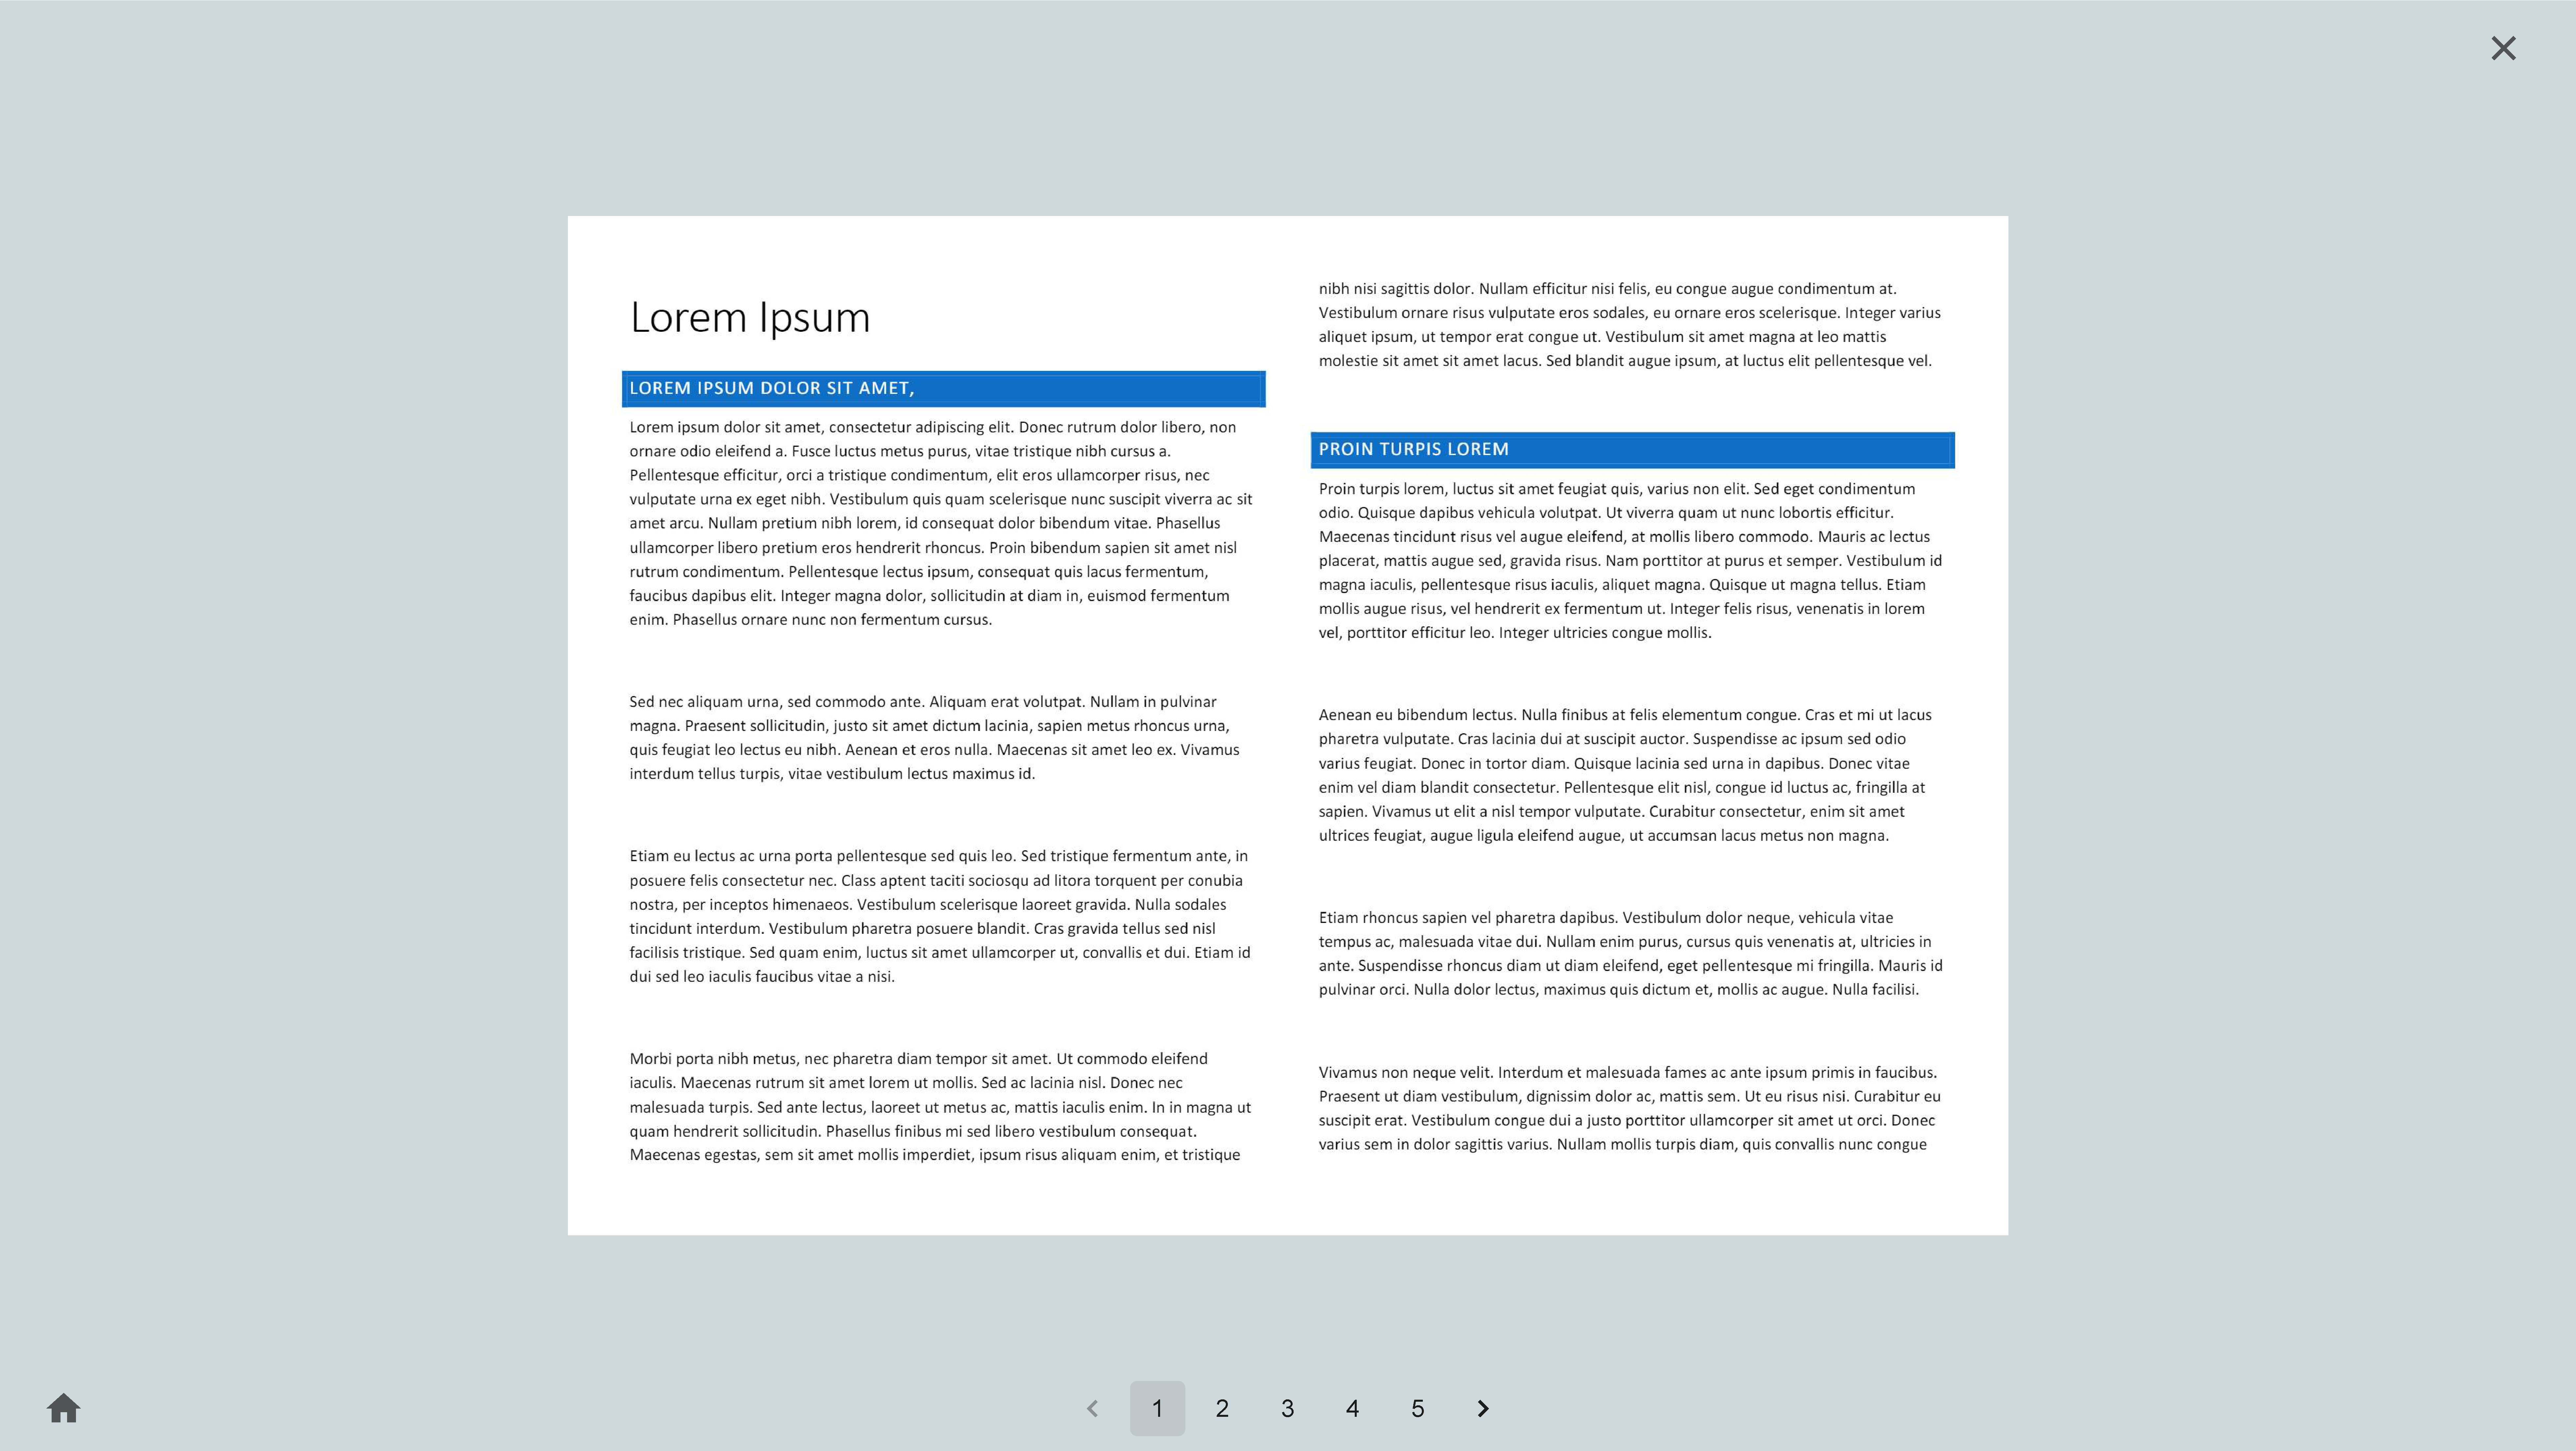
\includegraphics[width=.96\linewidth]{Figures/LUI/UI/documents-fullscreen.pdf}  
        \vspace{-5pt}
        \captionsetup{width=.9\linewidth}
        \caption{Documents app (item).}
        \label{fig:lui:screenshots:documents-fullscreen}
    \end{subfigure}

    \begin{subfigure}{.47\textwidth}
        \centering
        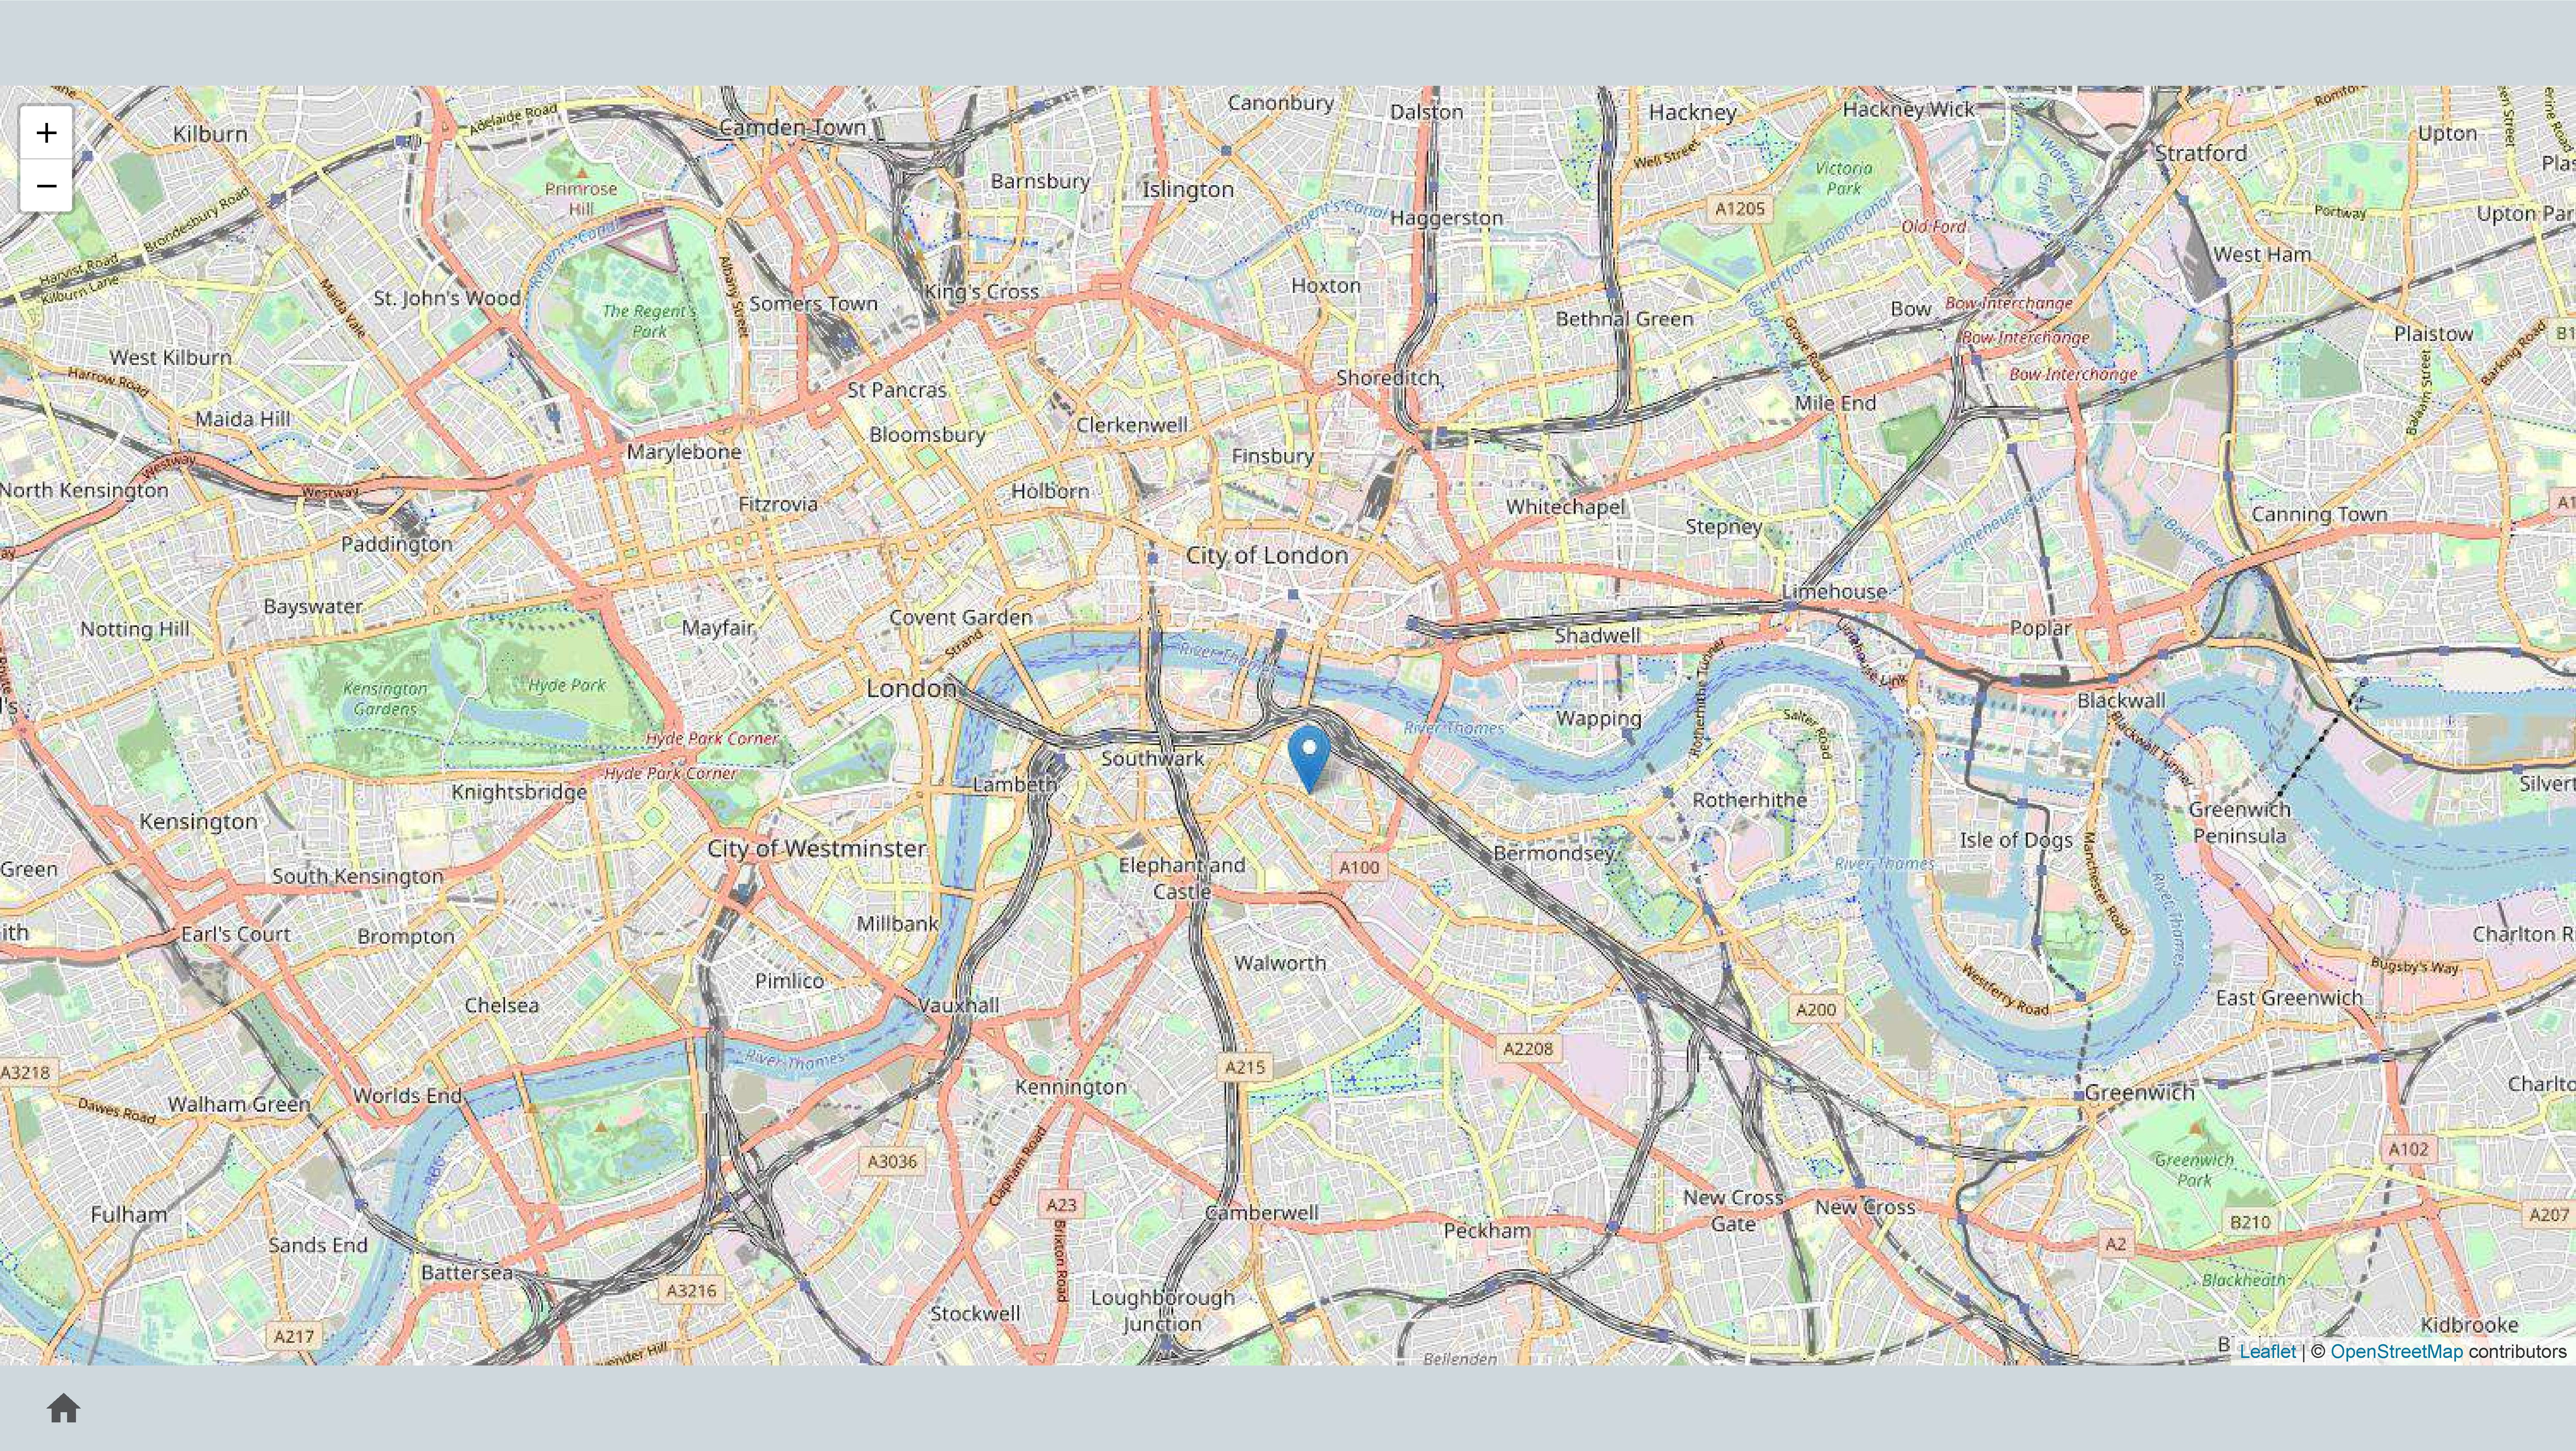
\includegraphics[width=.96\linewidth]{Figures/LUI/UI/maps.pdf} 
        \vspace{-5pt}
        \captionsetup{width=.9\linewidth}
        \caption{Maps app.}
        \label{fig:lui:screenshots:maps}
    \end{subfigure}
    \begin{subfigure}{.47\textwidth}
        \centering
        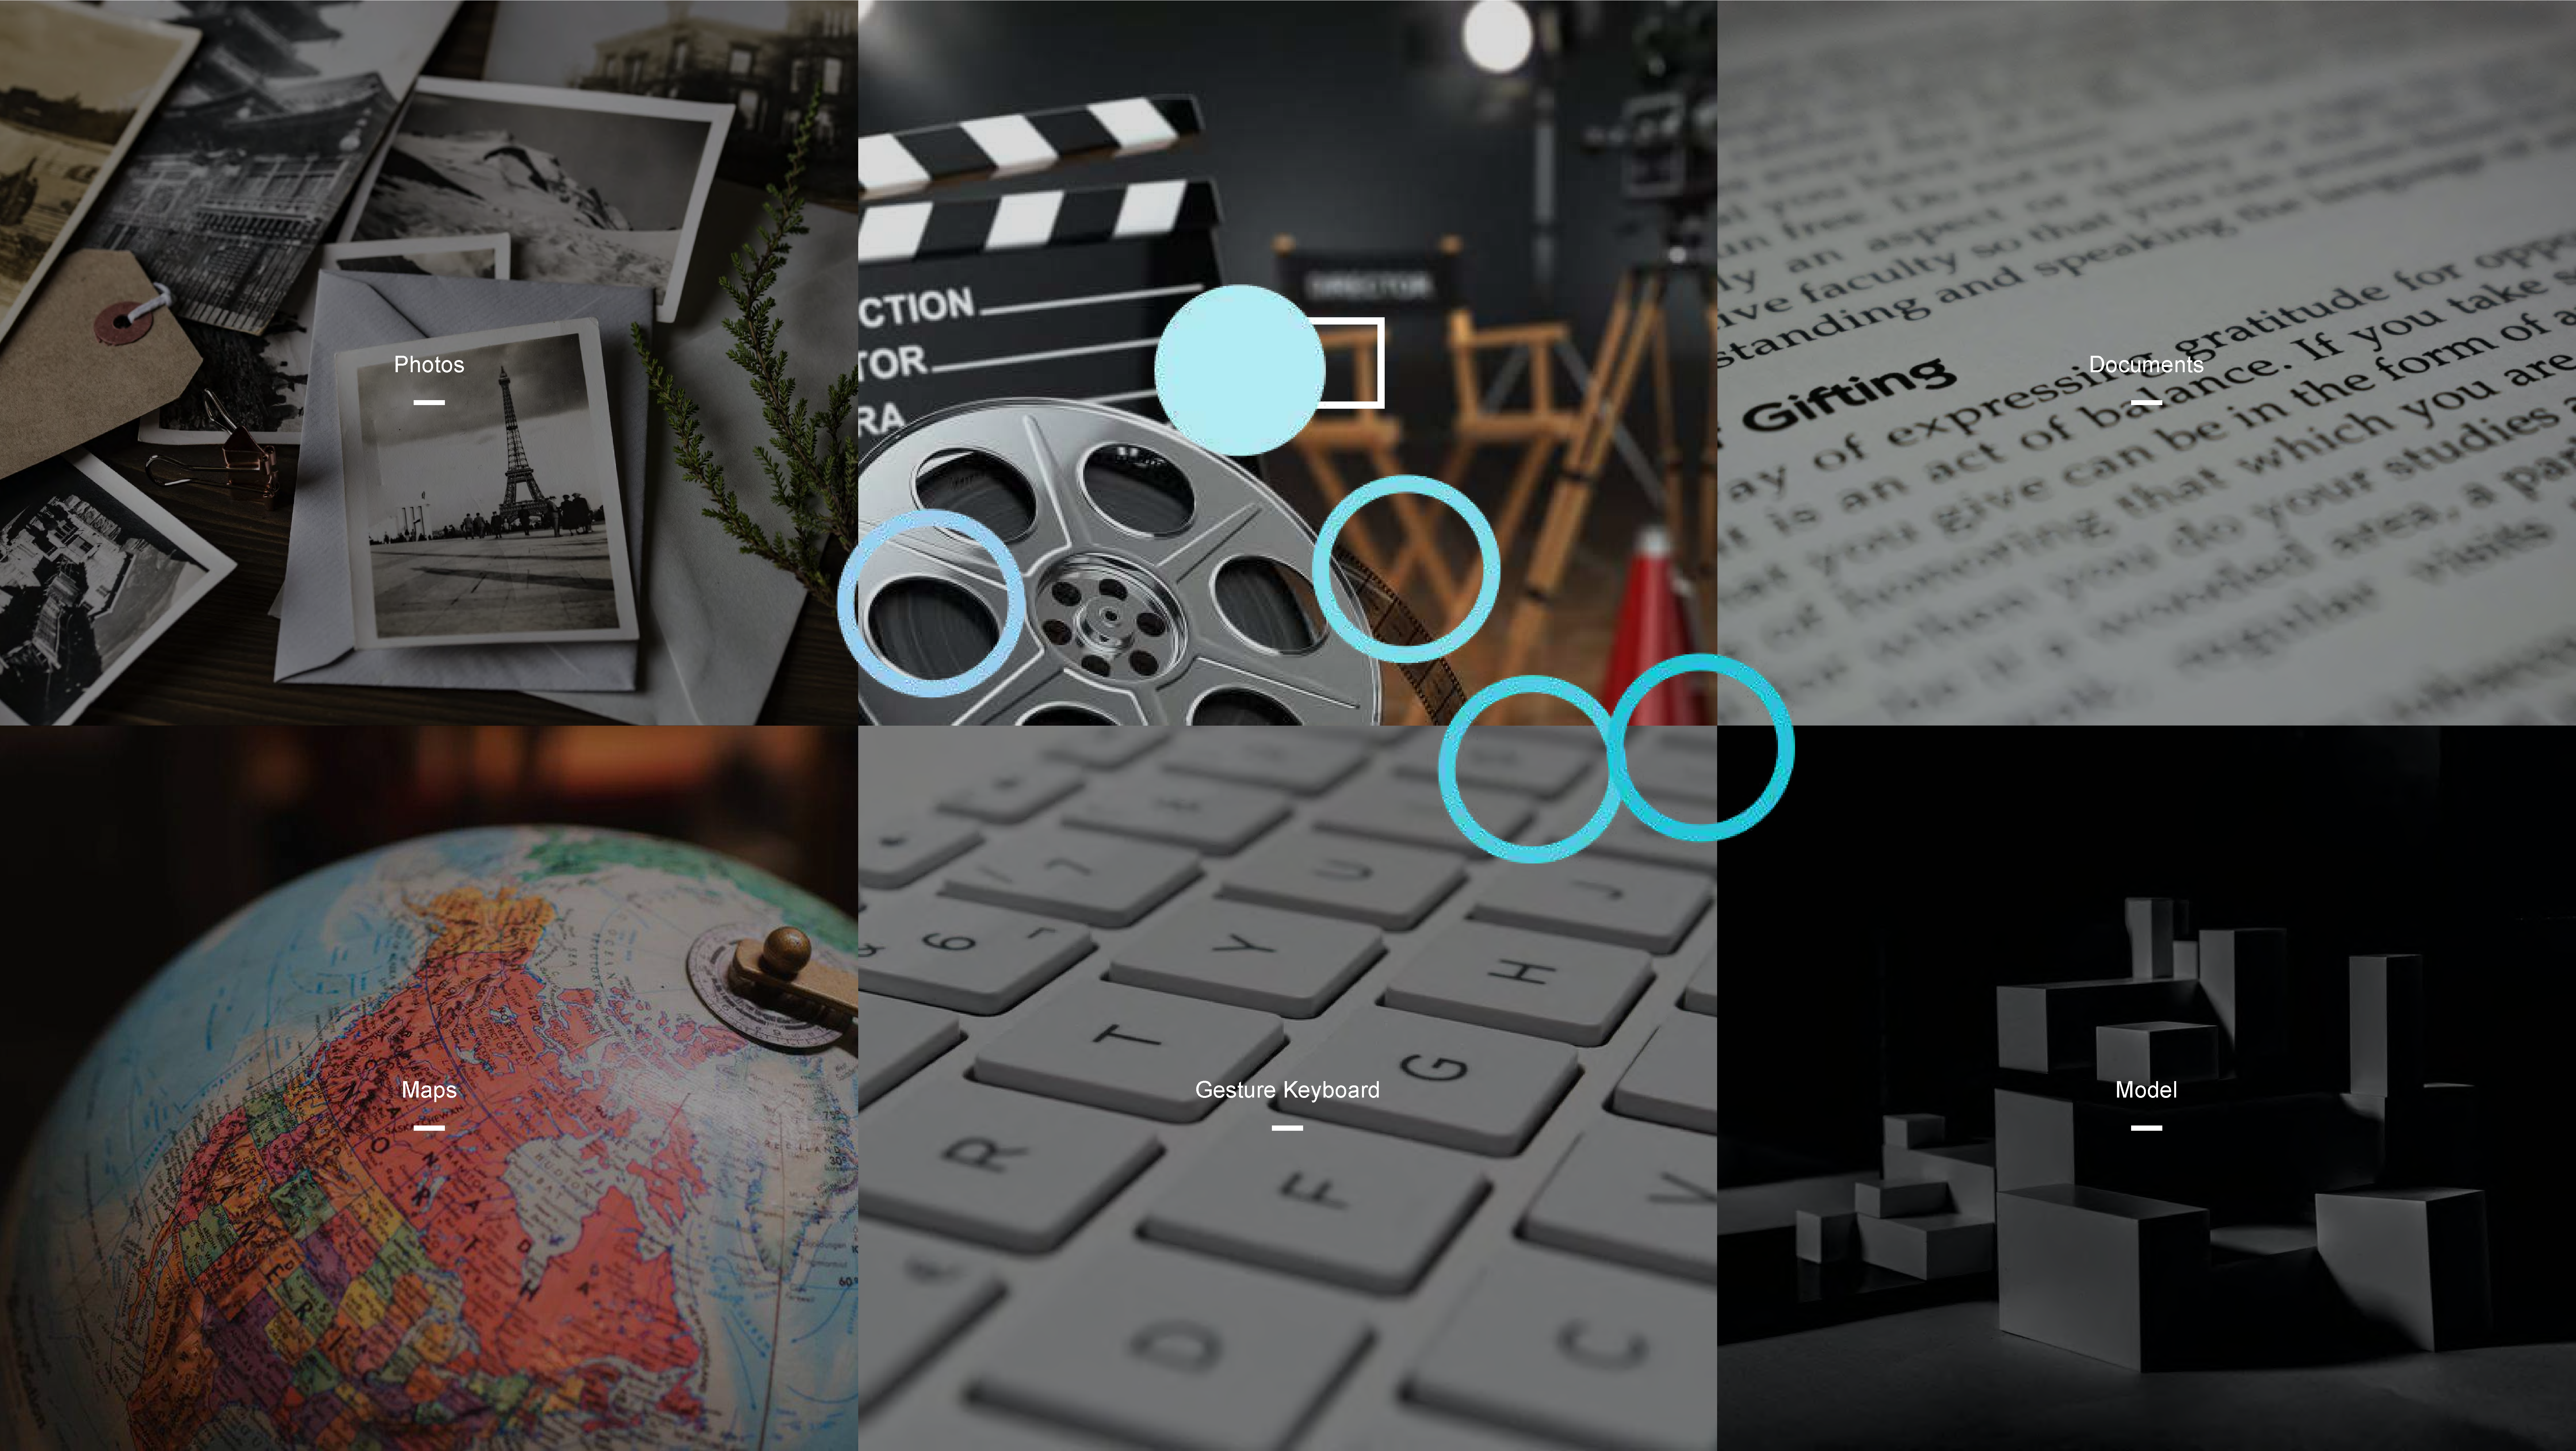
\includegraphics[width=.96\linewidth]{Figures/LUI/UI/fingers.pdf} 
        \vspace{-5pt}
        \captionsetup{width=.9\linewidth}
        \caption{User's hand.}
        \label{fig:lui:screenshots:hand}
    \end{subfigure}
    
    \vspace{-4pt}
    \caption{Screenshots of the third prototype of the \lui application.}
    % \vspace{-14pt}
    \label{fig:lui:screenshots}
\end{figure}

%--------------------------------------------------------------------------------%
\subsection{Requirements} \label{sec:lui:description:requirements}
To address the quality of the gesture interaction, \lui should fulfill three requirements:

\begin{enumerate}[noitemsep]
    \item \textit{Consistency.} Similar gestures should be assigned consistently to similar functions, independently of the media type, to foster knowledge transfer~\cite{Dingler:2018}, to maximize gesture memorability, and to reduce the learning curve~\cite{Delamare:2019}. Distinguishable gestures should be assigned to other specific functions~\cite{Kohlsdorf:2013}.
    \item \textit{Continuity.} End users should be able to perform gestures continuously, without needing to notify the system when they are performing a gesture, \ie the system should continuously recognize gestures and distinguish intended gestures from parasitic motion with little to no user intervention. End users should be able to manipulate media objects directly with a reasonable system response time (\eg 1 sec for direct manipulation according to~\cite{Nielsen:1994}) and continuous feedback to the user~\cite{Aigner:2012} (\eg gradually zooming in a picture by increasing the distance between the index and the thumb). Whether a gesture is discrete for a 0D/1D function or continuous for a 2D/3D function, this should not induce any difference for the end user.
    \item \textit{Customizability.} The system should support users in including their own gestures without requiring any modification to the \lui core~\cite{Coyette:2007}. User-defined gesture sets~\cite{Grijincu:2014} usually result in higher satisfaction and memorability than system- or designer-defined gestures~\cite{Nacenta:2013}. Some gesture recognizers perform better when the gestures used for training are recorded by the target user of the system~\cite{Vatavu:2013}.
\end{enumerate}

%--------------------------------------------------------------------------------%
\subsection{Iterative Design} \label{sec:lui:description:iterative-design}
The \lui application went through two iterations before the final one described in this chapter. This section summarizes the three iterations of \lui and its gesture set (\fig~\ref{fig:lui:gesture-set-evolution}).

\begin{figure}[!b]
    \centering
    % \vspace{-6pt}
    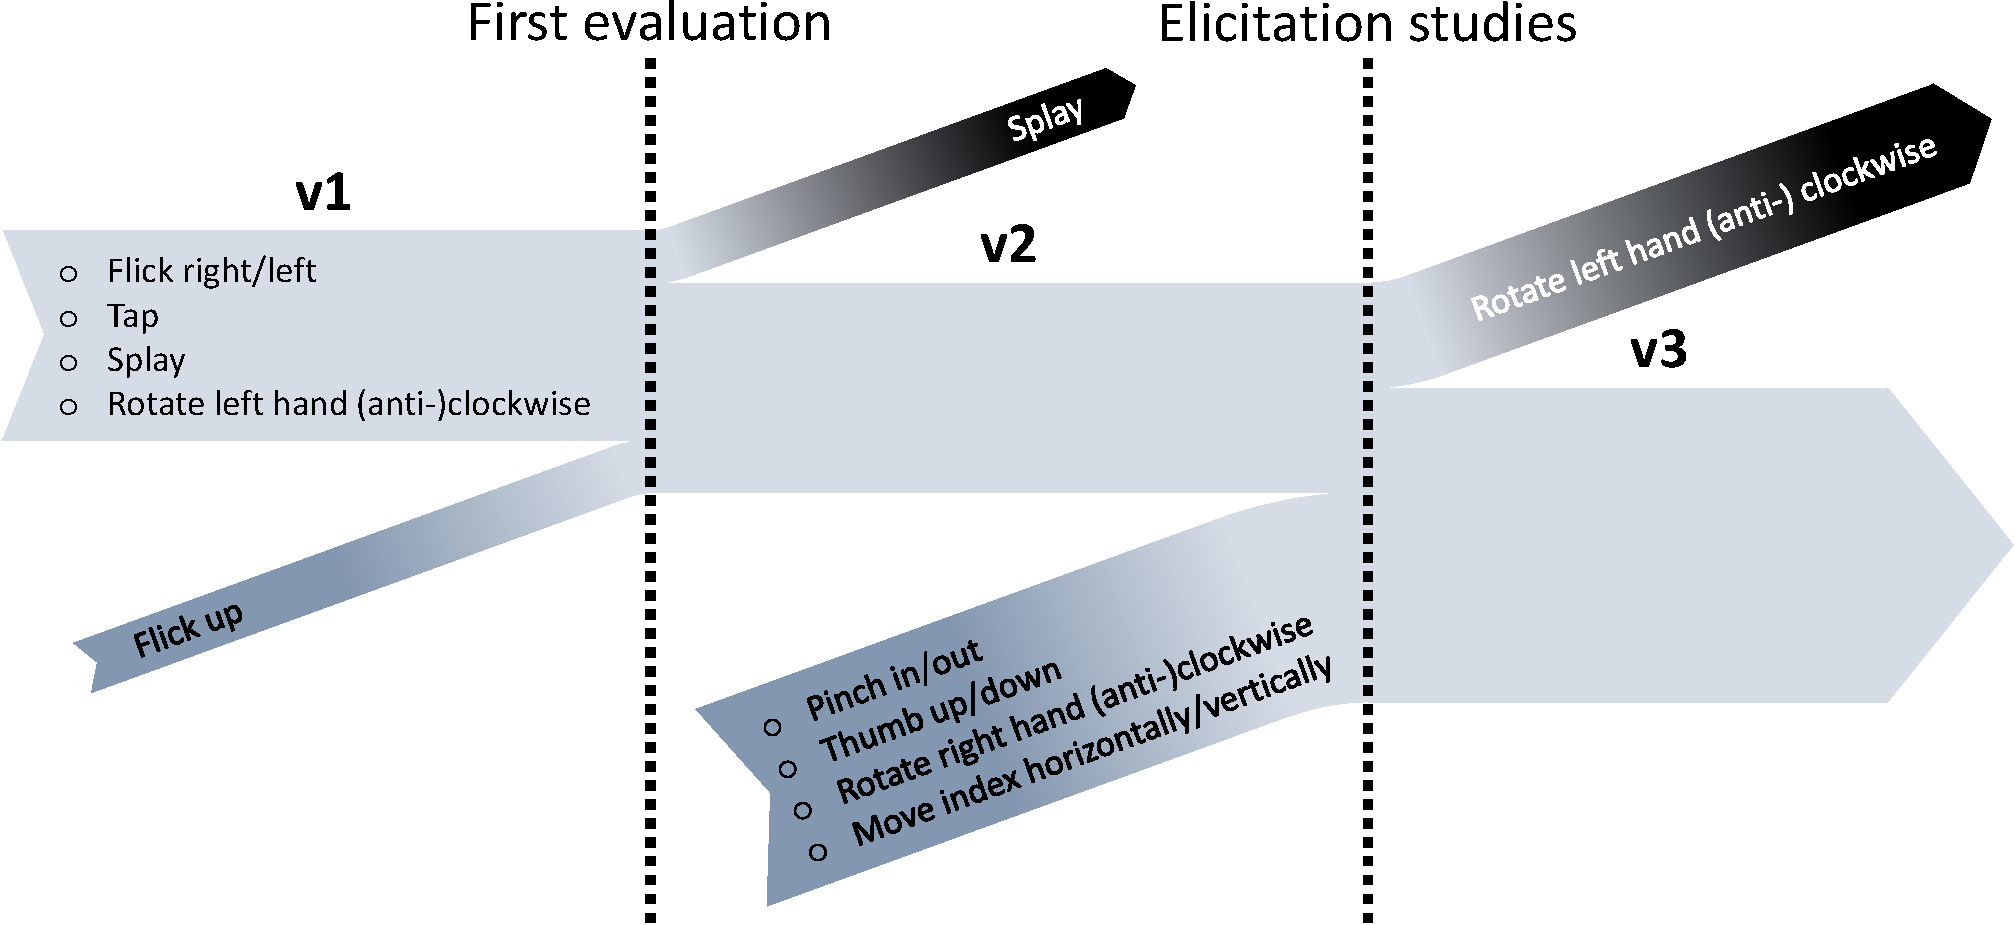
\includegraphics[width=\linewidth]{Figures/LUI/Overview/gesture-set-evolution.pdf}
    \vspace{-8pt}
    \caption{Evolution of the gesture set during the iterative design.}
    \label{fig:lui:gesture-set-evolution}
    % \vspace{-16pt}
\end{figure}

\subsubsection{First Iteration (v1)}
In this first prototype~\cite{Parthiban:2019}, the basics of \lui were laid out. Users could navigate through lists of photos and videos, switch to full-screen mode, and play, pause, or change the volume of a video. Gesture recognition was developed opportunistically based on the LMC API~\cite{Spiegelmock:2013}, which made adding new functions or gestures to \lui a complex endeavor and resulted in a rather small set of gestures. End users were thus forced to use the predefined gestures, with no possibility of assigning their own gestures to specific functions.

\subsubsection{Second Iteration (v2)}
A usability testing was conducted with 20 participants to evaluate their subjective satisfaction regarding the first prototype~\cite{Parthiban:2019,Dumas:2019}. It highlighted multiple issues, including a high learning curve, unpredictable gesture recognition, and fatigue, in particular for the \textit{splay} gesture, which participants found especially difficult to perform and reproduce accurately. 
Some participants expressed their intention to define their own preferred gestures, instead of using the predefined ones.
This second prototype replaced the \textit{splay} gesture with the \textit{flick up} gesture, which is easier to perform. Other issues highlighted by the testing were left unaddressed in this version, as they required more substantial modifications to the \lui core.

\subsubsection{Third Iteration (v3)}
The current version of \lui was developed based on the assets of the first two prototypes but features significant changes to its gesture set and gesture recognition pipeline (Section~\ref{sec:lui:development-method}). 
It now relies on the \ql pipeline for gesture recognition, which enables end users to add their own preferred gestures to predefined ones without having to modify the \lui core. The use of \ql also vastly simplified the process of extending \lui with new applications and gestures, which enabled us to add new functions to the Photos and Videos applications (\eg rotating a photo and browsing through a video), and implement new Documents and Maps applications.

%================================================================================%
\section{User-centered Development Method} \label{sec:lui:development-method}
This section details the three-stage development process that we followed for the third iteration of \lui. 
%
We first designed an intuitive set of gestures, consistent across the entire \lui application, based on the results of a GES. 
%
Then, we ran a comparative testing of static and dynamic gesture recognizers using the \ql testing tool (Chapter~\ref{chap:quantumleap-testing}) to identify a suitable dataflow configuration for this gesture set.
%
Finally, we instantiated a gesture recognition dataflow based on the results of our testing using the \ql framework (Chapter~\ref{chap:quantumleap}).

%--------------------------------------------------------------------------------%
\subsection{Gesture Set Design} \label{sec:lui:development-method:gesture-set}
\subsubsection{Gesture Identification}
As the number of functions increased, it was decided to conduct a GES~\cite{Wobbrock:2009} to explore a consensus set of consistent gestures that would optimize agreement among end users. Based on the classical method~\cite{Wobbrock:2009} and some extensions~\cite{Gheran:2018}, we initially conducted two GESs (see Appendix~\ref{app:lui-ges:initial}): one for photo browsing and another for video browsing. Prior work~\cite{Anthony:2013,Groenewald:2016} pointed out that gesture sets for different devices could be inconsistent. Our two studies confirm this observation as they led to inconsistent gestures tailored to one media type at a time. 
Rather than conducting a separate GES for each media type, we conducted a single GES (see Appendix~\ref{app:lui-ges:new}) integrating the various media with both generic and specific functions.

The result of our GES consists of a characterization of users' gesture input behaviors with valuable information for designers, practitioners, and end users regarding the consensus among participants (which is computed as an \textit{agreement} and \textit{co-agreement rate}~\cite{Vatavu:2015}), most frequent (thus, generalizable across users) gestures for a specified task, and insights into users' conceptual models for performing tasks. \cite{Dingler:2018} computed the agreement score~\cite{Wobbrock:2009} for their multi-device GES. Instead, we computed the agreement rate $AR(r)$~\cite{Vatavu:2015}, which is smaller and more restrictive than the agreement score $A(r)$, as follows:
\vspace{-5pt}
\begin{equation}
A(r) = \sum_{P_i \subseteq P} {\Bigg( \frac{\lvert P_i \vert}{\lvert P \vert} \Bigg)}^2
\geq
AR(r)= \frac{
\sum_{P_i\subseteq P} {\frac{1}{2} \lvert P_i \vert  \:(\lvert P_i \vert{-}1)}}
{\frac{1}{2} \lvert P \vert   \:(\lvert P \vert{-}1)}
\label{eq:agreement1}
\end{equation}
%\vspace{-3pt}
where $r$ denotes the referent to elicit a gesture, $\lvert P \rvert$ denotes the number of elicited gestures, and $\vert P_{i} \rvert$ denotes the number of gestures elicited for the $i^{th}$ subgroup of $P$. 


\tab~\ref{tbl:lui-ges:gesture-proposals} summarizes the two most agreed gestures for each referent of the GES. 
% One-handed
From these results, we observe that the majority ($\frac{16}{18} {=} 88.9\%$) of the most agreed gestures were one-handed. One-handed gestures let users interact with the system while holding an object in the other hand (\eg a glass of water or a paper document). In addition, the low occurrence of two-handed gestures in our study may be explained by a lower ease of execution compared to one-handed gestures~\cite{Morris:2010}.
% User-defined gestures + indirect method
Some referents, such as enable/disable subtitles, have a very low agreement rate. For these referents, user-elicited gestures may not be the most appropriate, as the low consensus may result in lower guessability and memorability~\cite{Wobbrock:2005}. Instead, it may be preferable to favor other solutions, such as prompting users to assign their own gesture to these actions at the start of the application (\ie user-defined gestures~\cite{Nacenta:2013}), and/or providing an indirect way of triggering these actions (\eg by navigating through a menu with highly agreed gestures).
% Aliasing
For referents with a low to medium agreement rate, such as play and pause, aliasing (\ie assign multiple gestures, such as the most and second most agreed gestures, to one referent) may greatly increase guessability~\cite{Wobbrock:2005, Wobbrock:2009}. This would enable users to use the gesture they are most familiar with, and thus flatten the learning curve and increase the memorability of the gesture set. However, attentive care should be given to avoid overloading gestures.

\begin{figure}[ht]
    \begin{subfigure}{.24\textwidth}
        \centering
        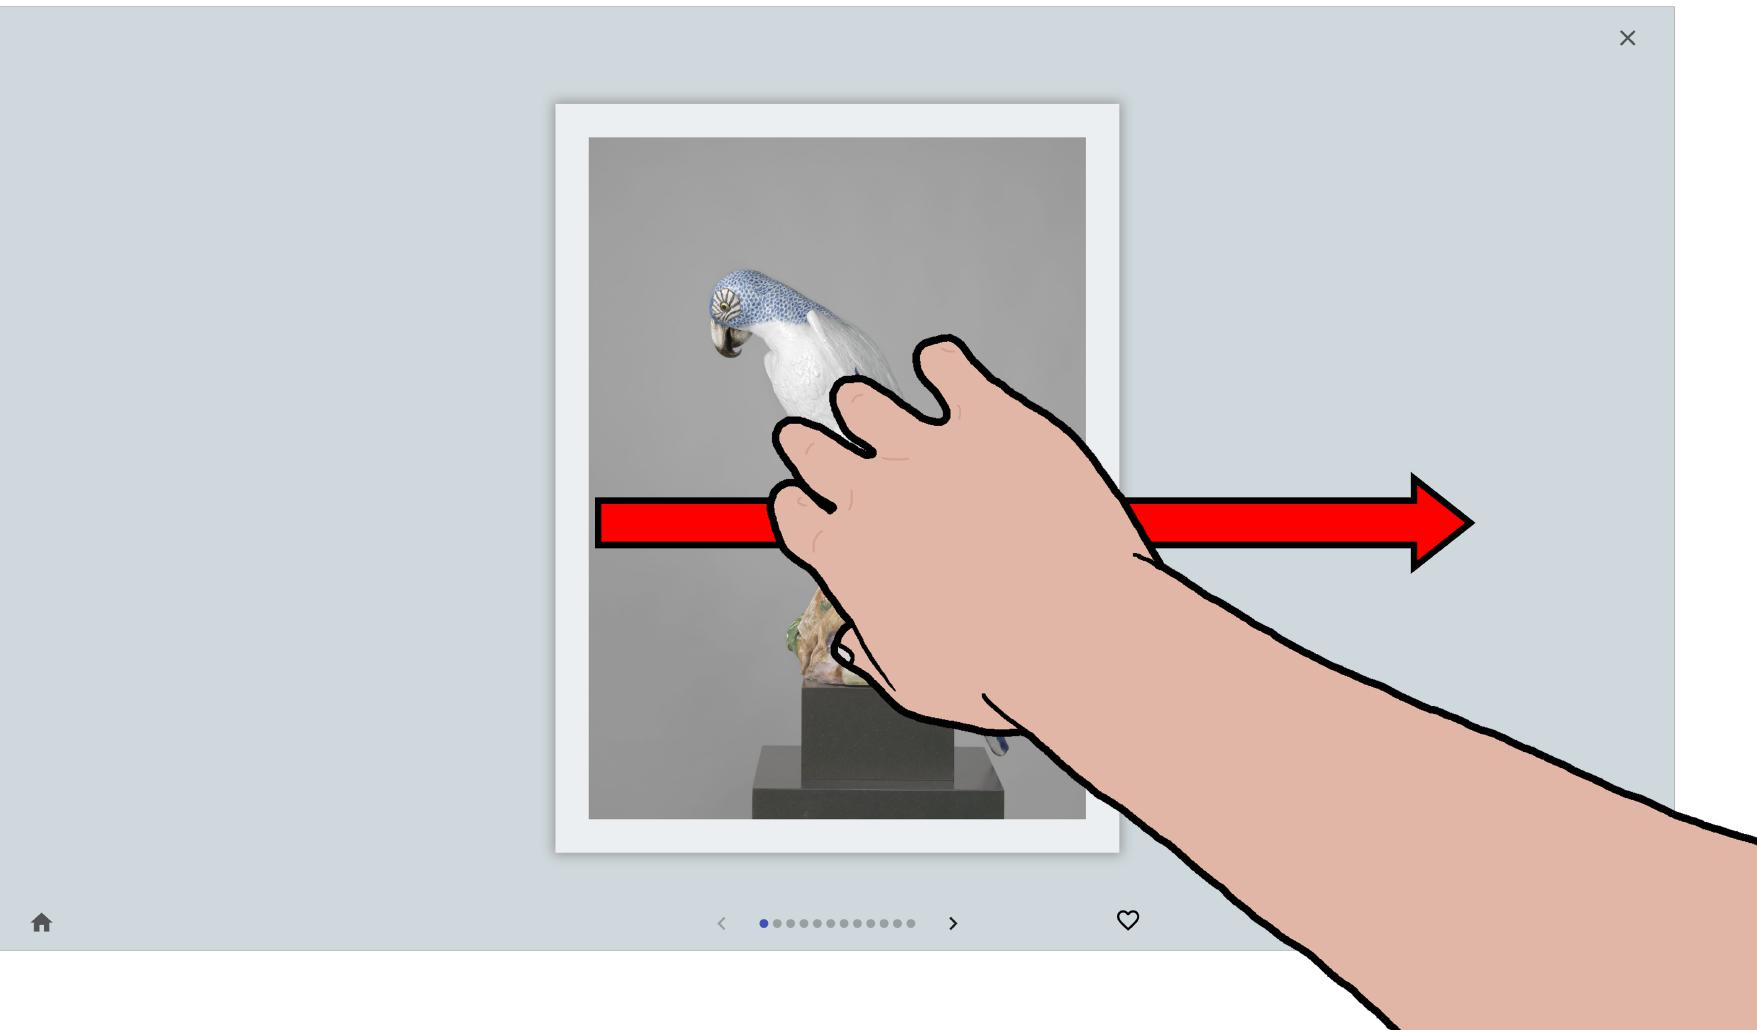
\includegraphics[width=.97\linewidth]{Figures/LUI/Gestures/flick_right.pdf}  
        \vspace{-6pt}
        \captionsetup{width=.9\linewidth}
        \caption{Previous.}
        \label{fig:lui:gestures:previous}
    \end{subfigure}
    \begin{subfigure}{.24\textwidth}
        \centering
        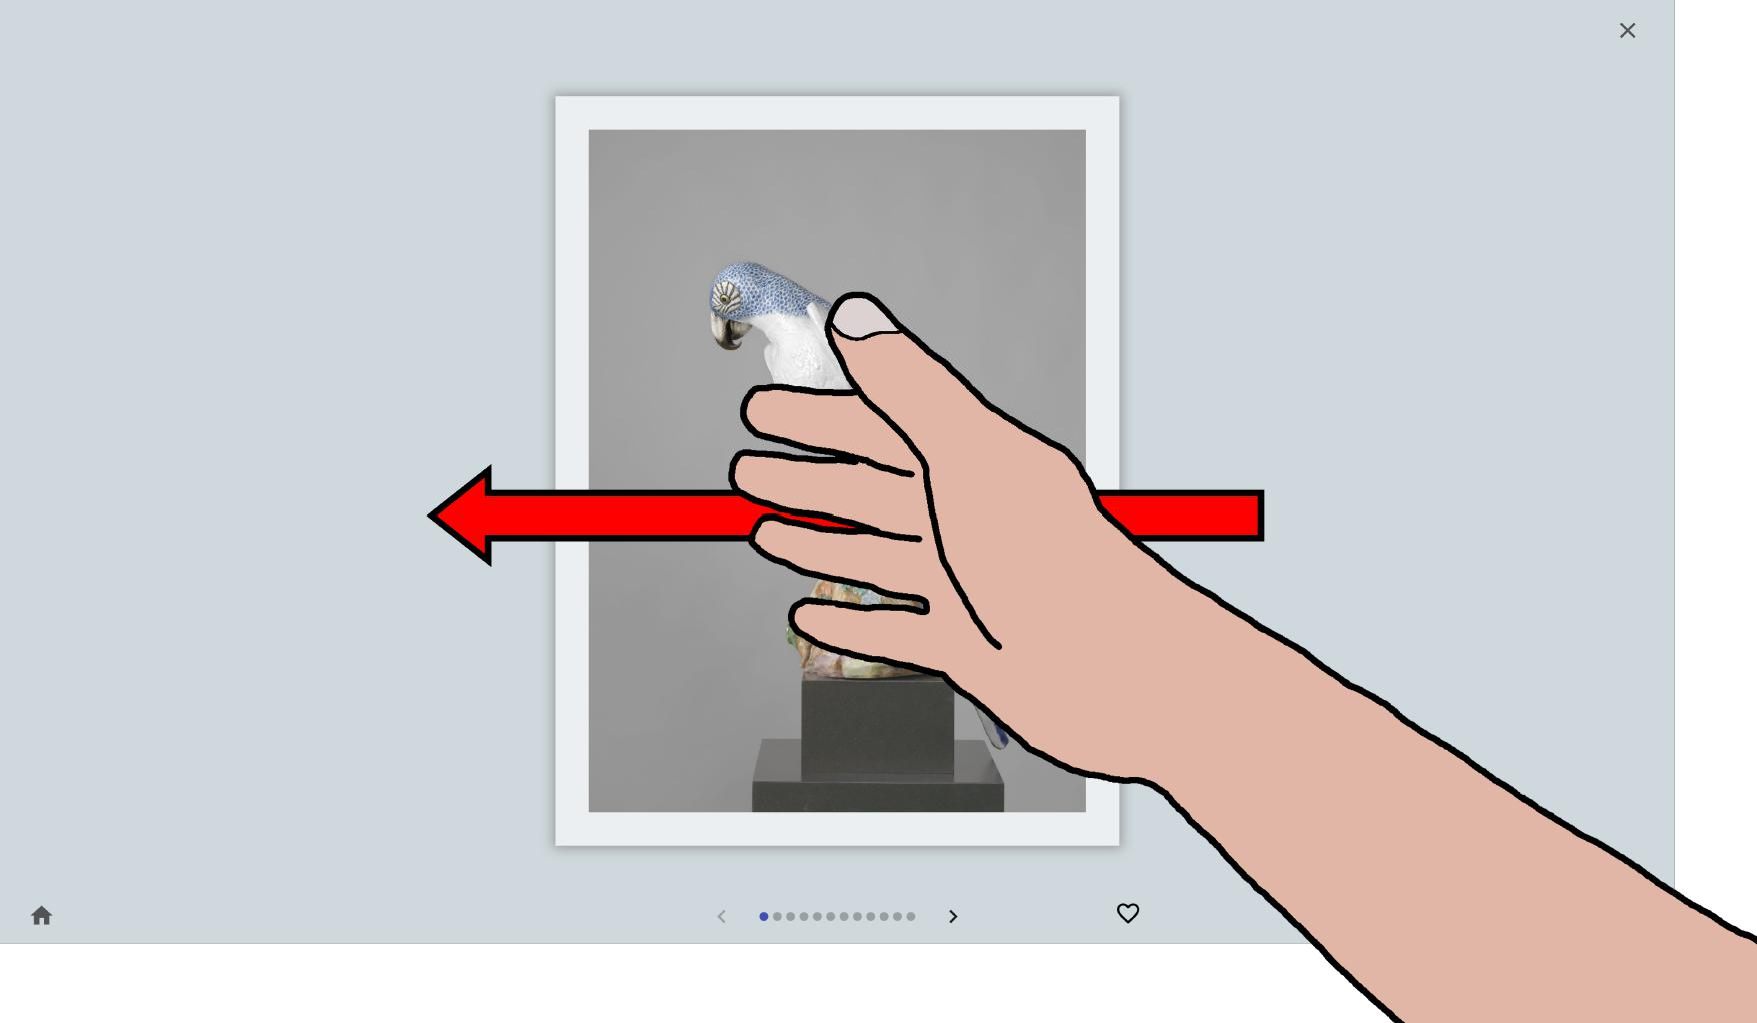
\includegraphics[width=.97\linewidth]{Figures/LUI/Gestures/flick_left.pdf}  
        \vspace{-6pt}
        \captionsetup{width=.9\linewidth}
        \caption{Next.}
        \label{fig:lui:gestures:next}
    \end{subfigure}
    \begin{subfigure}{.24\textwidth}
        \centering
        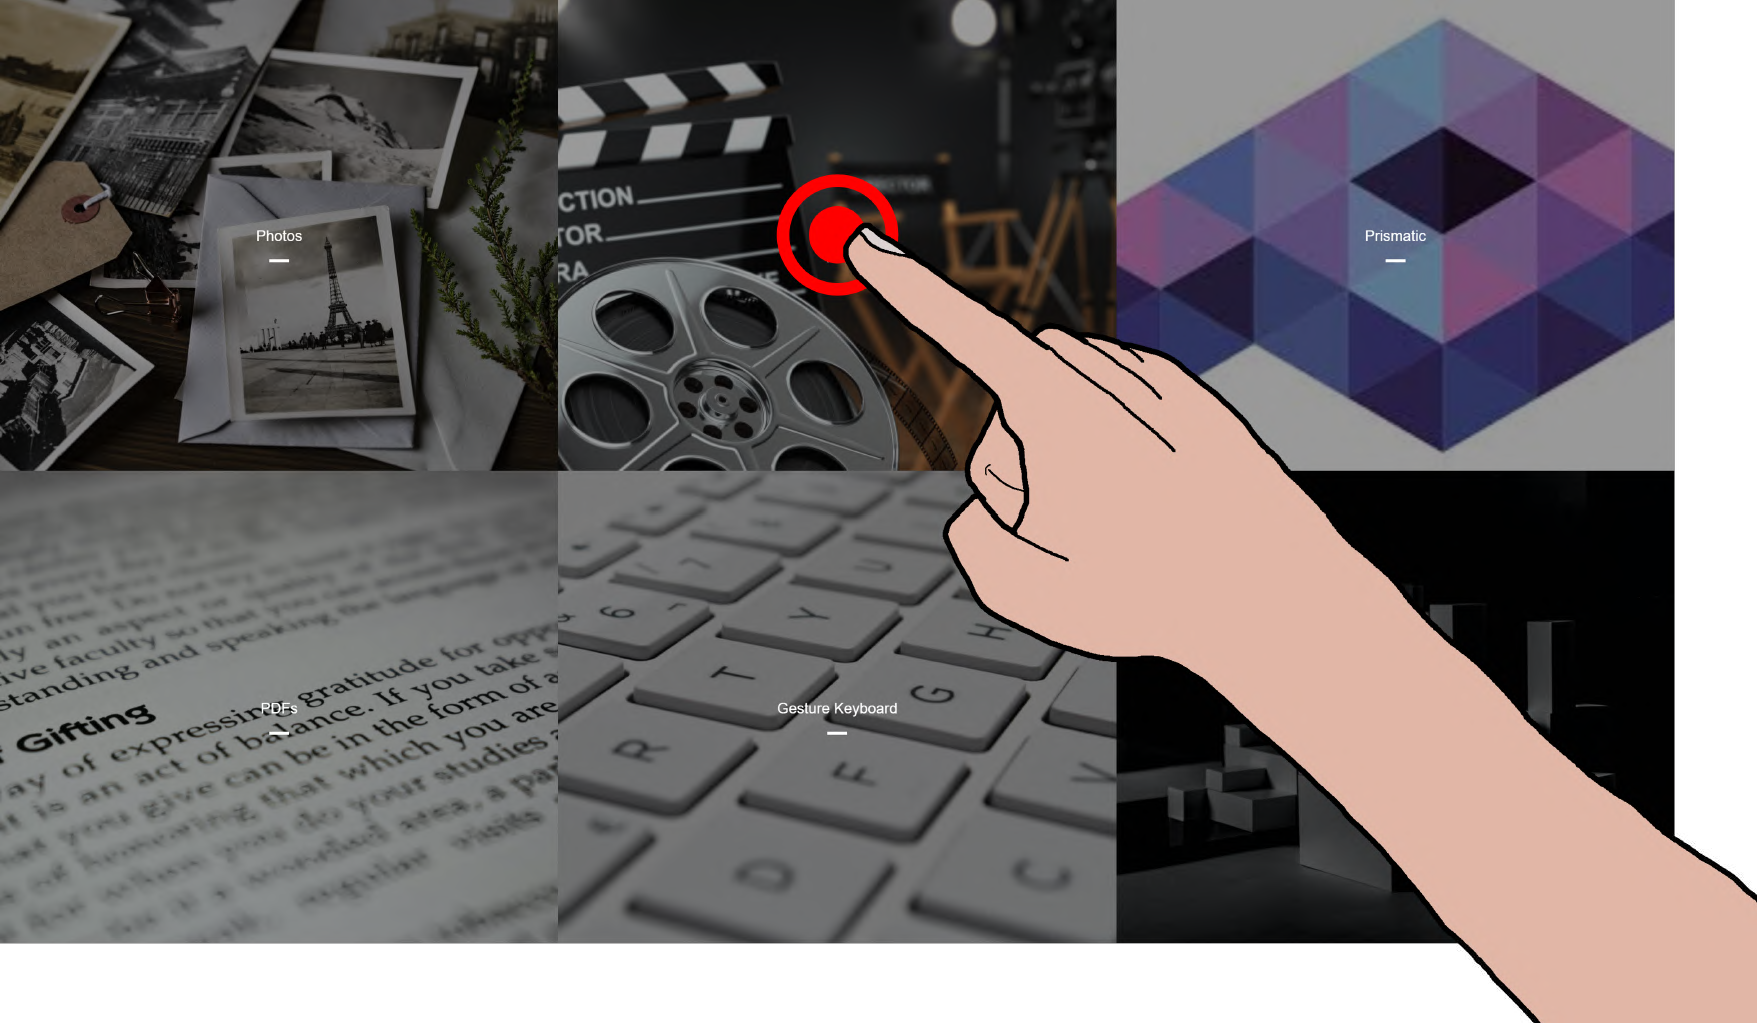
\includegraphics[width=.97\linewidth]{Figures/LUI/Gestures/tap-open.pdf} 
        \vspace{-6pt}
        \captionsetup{width=.99\linewidth}
        \caption{Enable fullscreen.}
        \label{fig:lui:gestures:fullscreen-on}
    \end{subfigure}
    \begin{subfigure}{.24\textwidth}
        \centering
        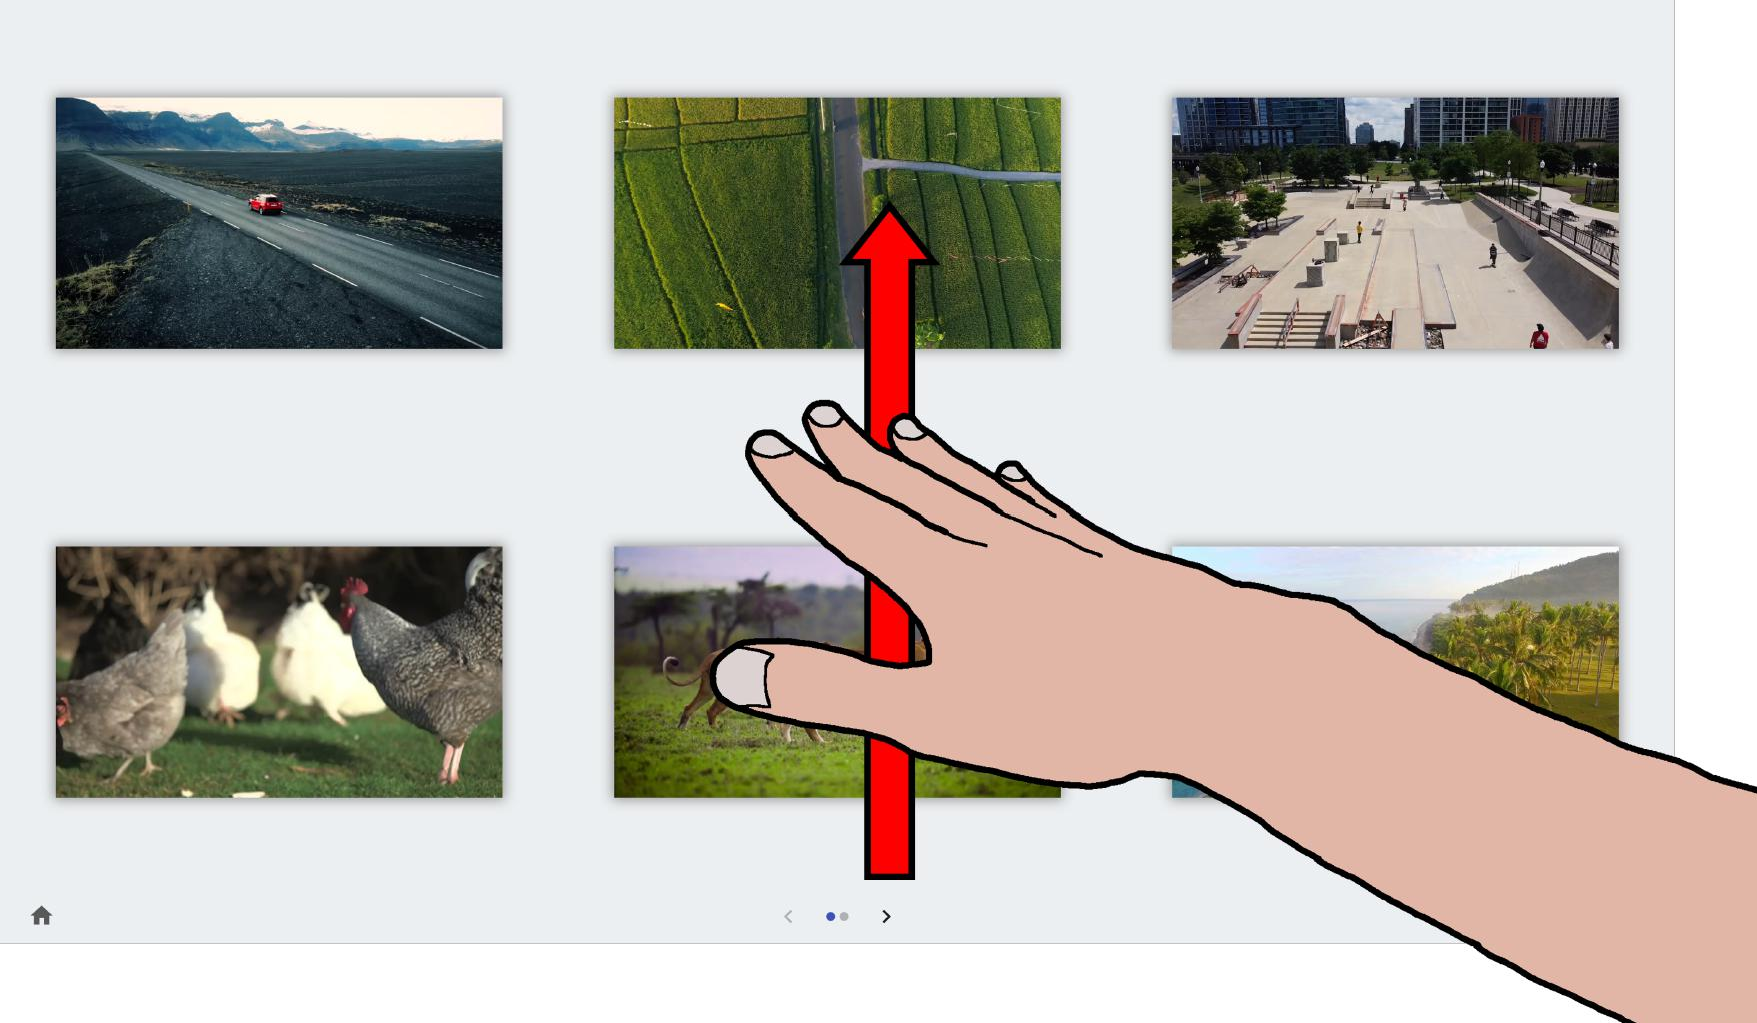
\includegraphics[width=.97\linewidth]{Figures/LUI/Gestures/flick_up.pdf} 
        \vspace{-6pt}
        \captionsetup{width=.99\linewidth}
        \caption{Disable fullscreen.}
        \label{fig:lui:gestures:fullscreen-off}
    \end{subfigure}
    
    \begin{subfigure}{.24\textwidth}
        \centering
        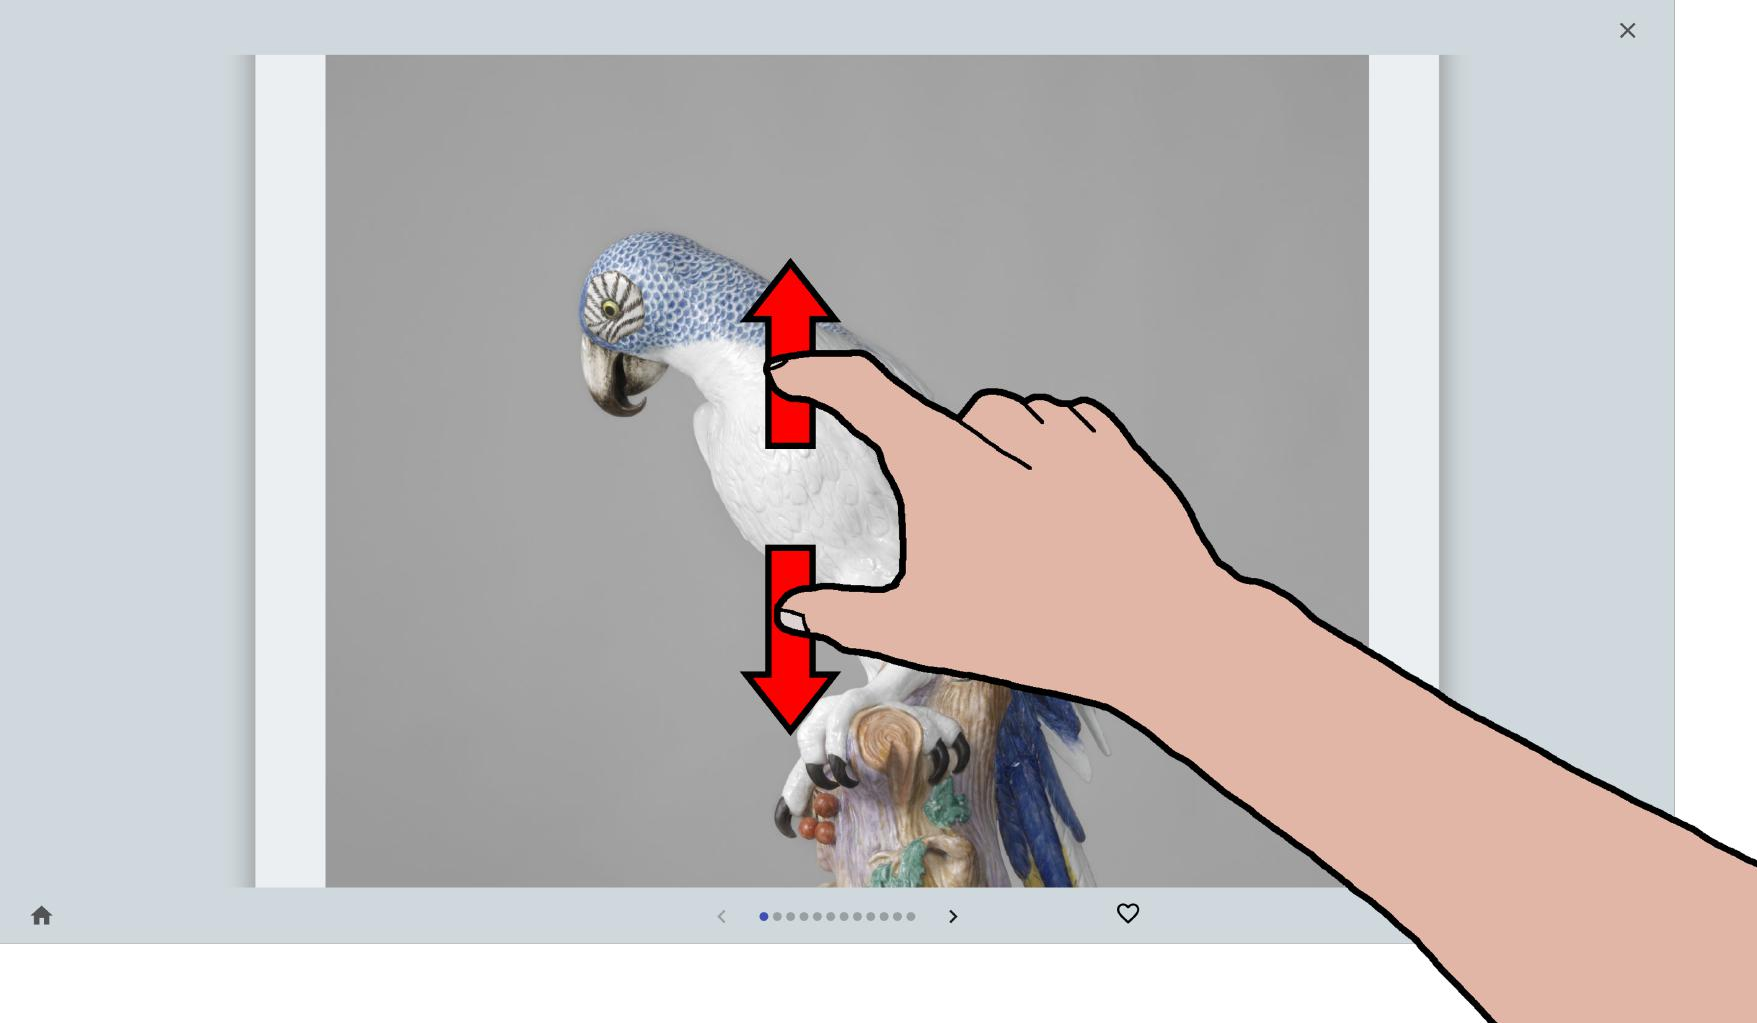
\includegraphics[width=.97\linewidth]{Figures/LUI/Gestures/pinch_out.pdf}
        \vspace{-6pt}
        \captionsetup{width=.9\linewidth}
        \caption{Zoom in.}
        \label{fig:lui:gestures:zoom-in}
    \end{subfigure}
    \begin{subfigure}{.24\textwidth}
        \centering
        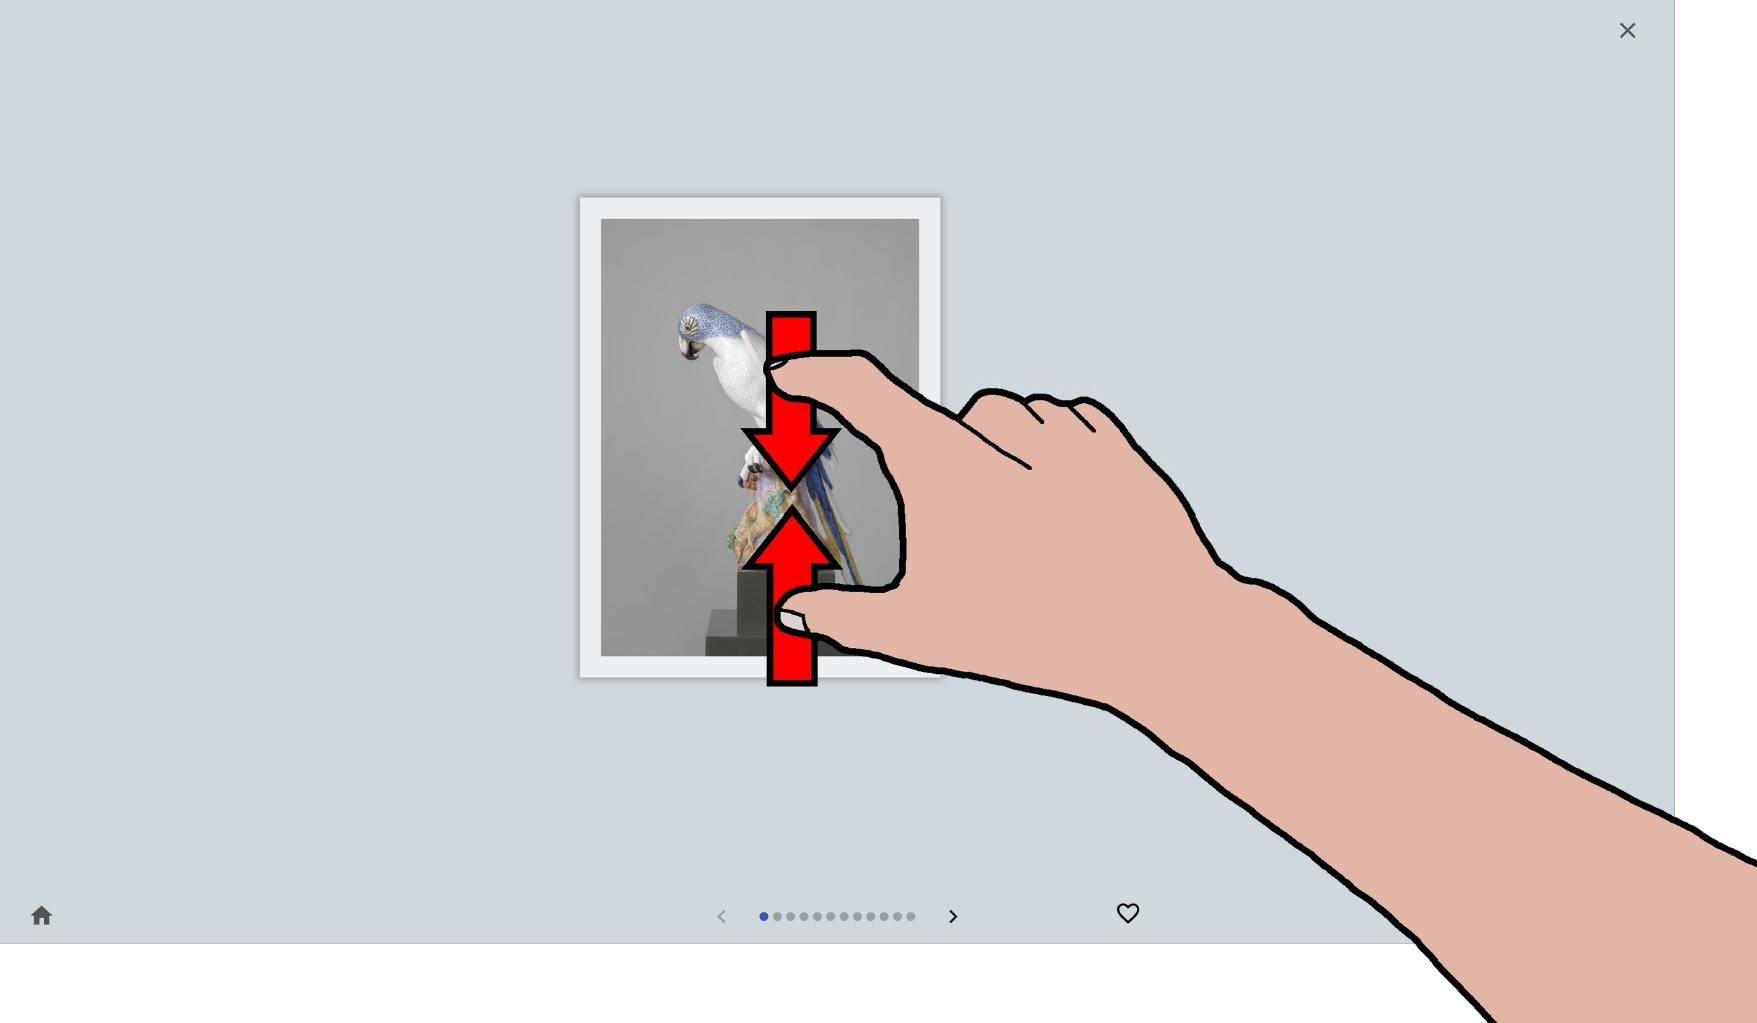
\includegraphics[width=.97\linewidth]{Figures/LUI/Gestures/pinch_in.pdf} 
        \vspace{-6pt}
        \captionsetup{width=.9\linewidth}
        \caption{Zoom out.}
        \label{fig:lui:gestures:zoom-out}
    \end{subfigure}
    \begin{subfigure}{.24\textwidth}
        \centering
        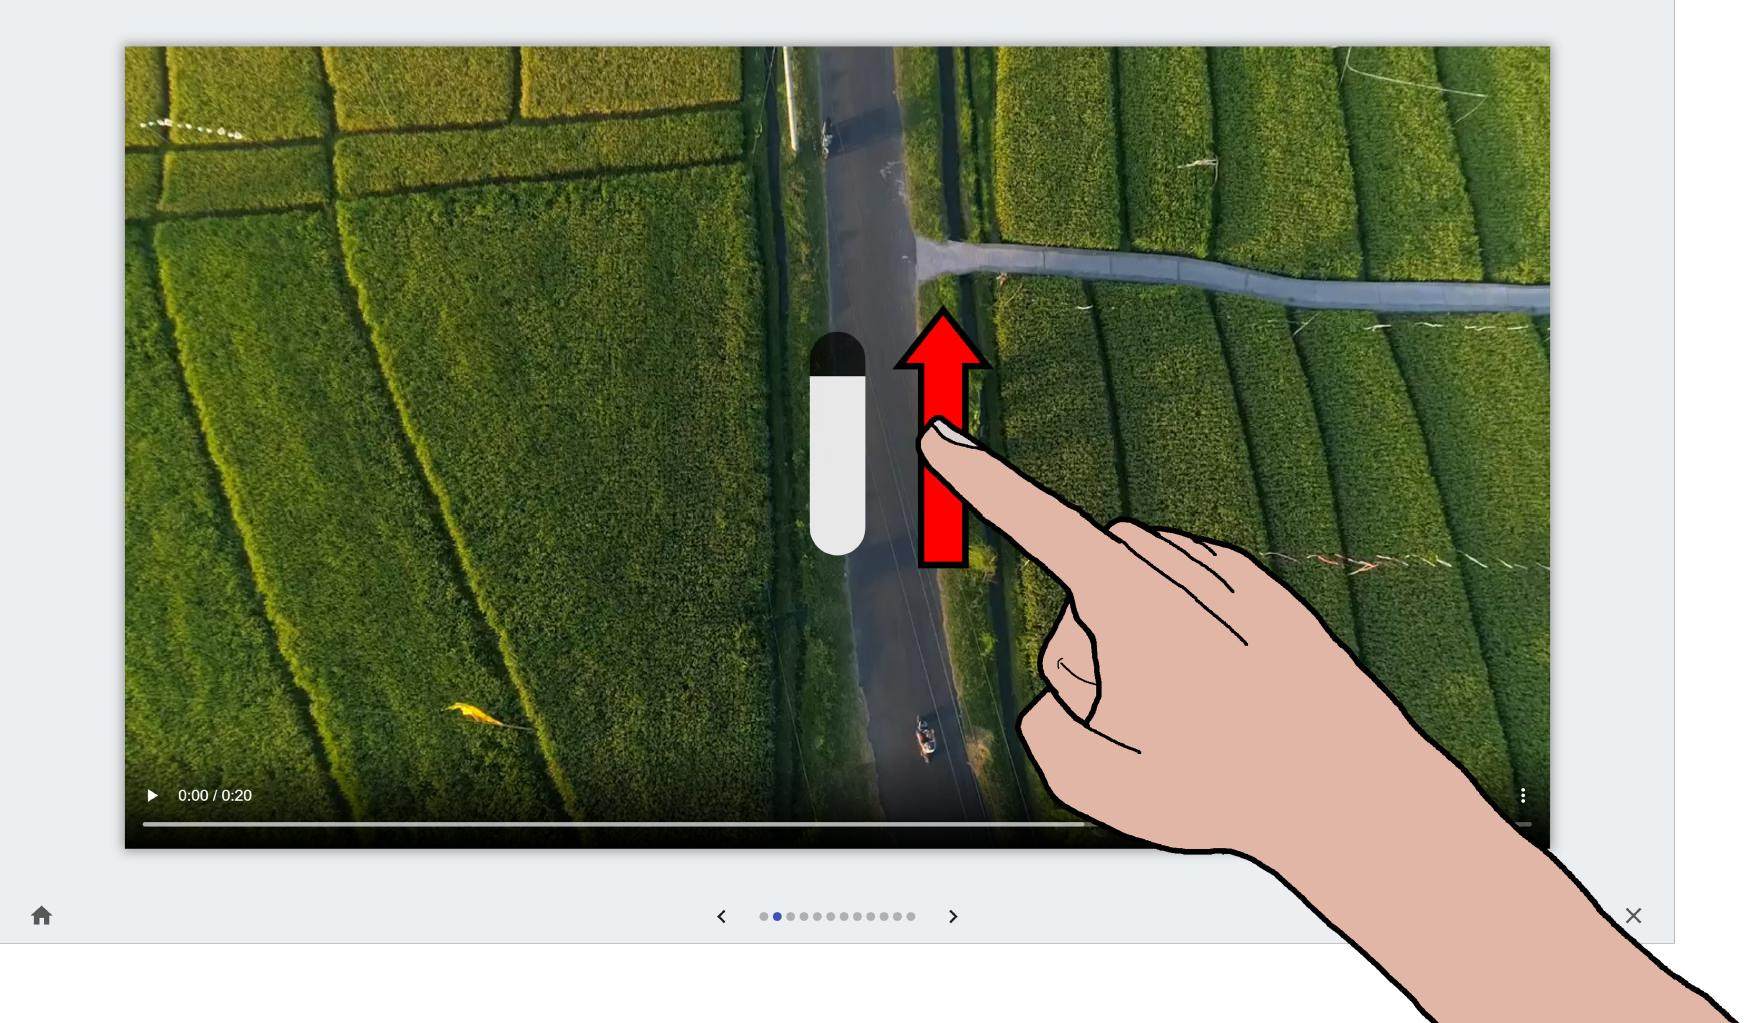
\includegraphics[width=.97\linewidth]{Figures/LUI/Gestures/swipe_up-volume.pdf}  
        \vspace{-6pt}
        \captionsetup{width=.9\linewidth}
        \caption{Volume up.}
        \label{fig:lui:gestures:volume-up}
    \end{subfigure}
    \begin{subfigure}{.24\textwidth}
        \centering
        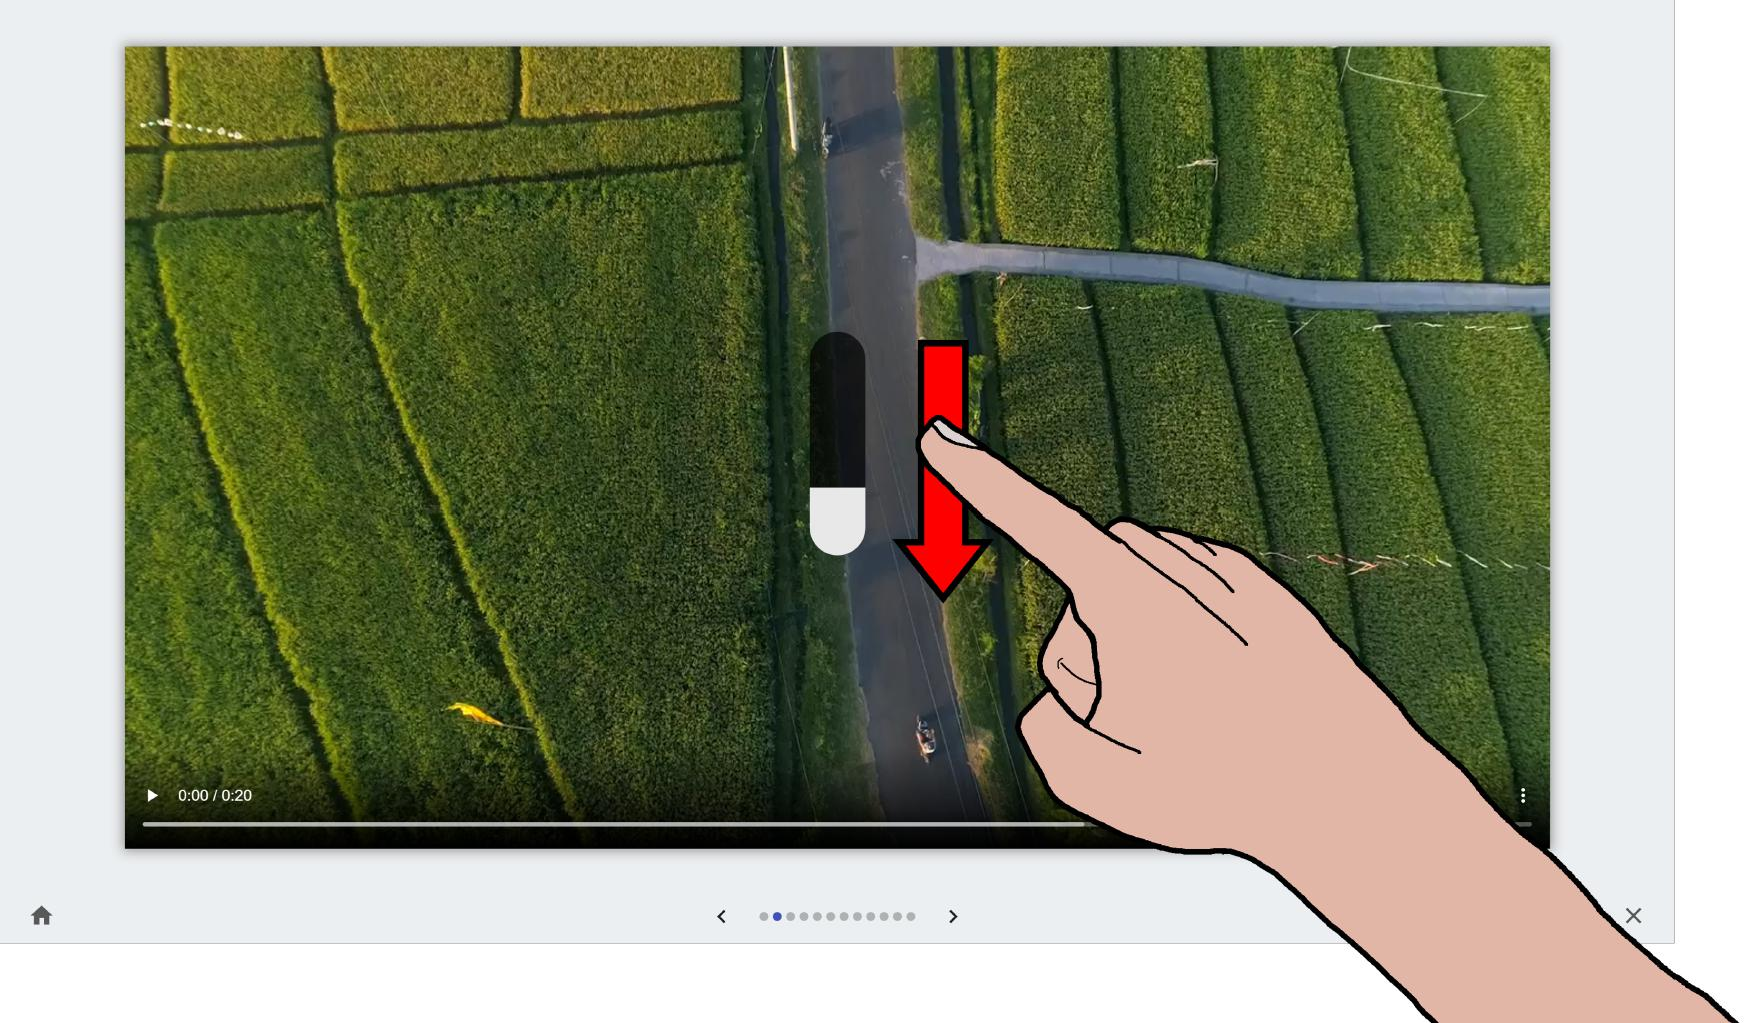
\includegraphics[width=.97\linewidth]{Figures/LUI/Gestures/swipe_down-volume.pdf}  
        \vspace{-6pt}
        \captionsetup{width=.9\linewidth}
        \caption{Volume down.}
        \label{fig:lui:gestures:volume-down}
    \end{subfigure}

    \begin{subfigure}{.24\textwidth}
        \centering
        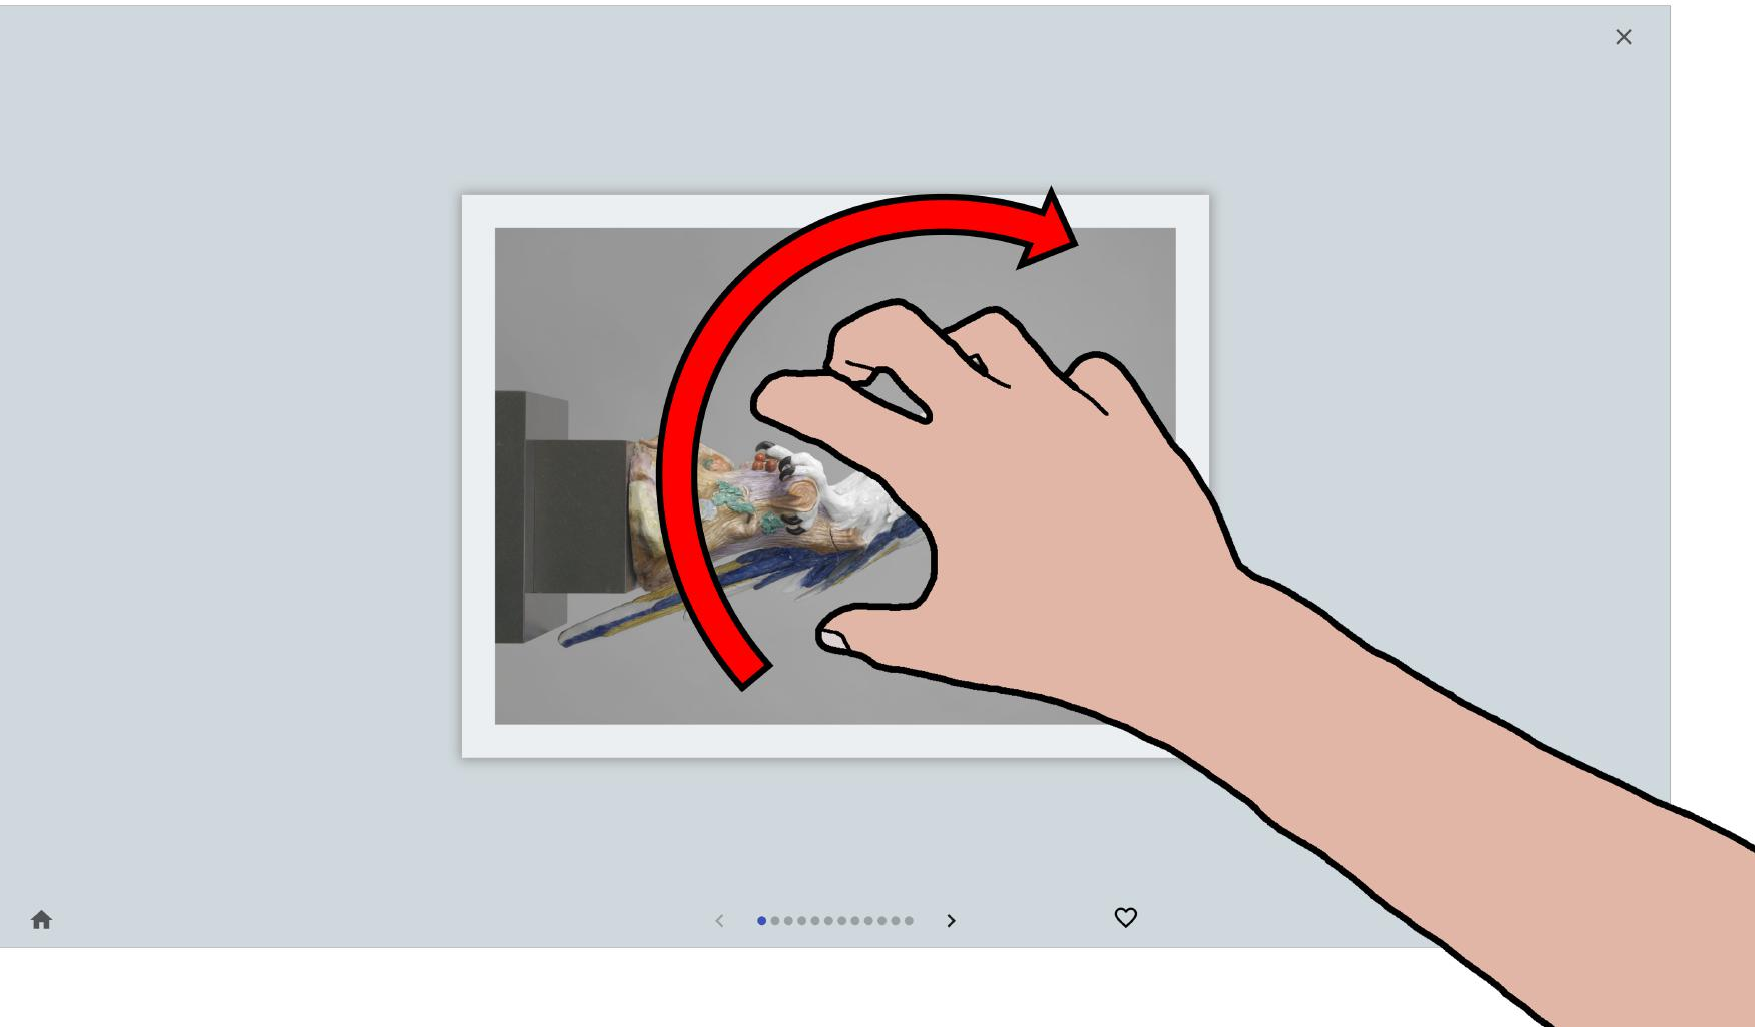
\includegraphics[width=.97\linewidth]{Figures/LUI/Gestures/rotate_clockwise.pdf}  
        \vspace{-6pt}
        \captionsetup{width=.9\linewidth}
        \caption{Rotate clockwise.}
        \label{fig:lui:gestures:rotate-anticlock}
    \end{subfigure}
    \begin{subfigure}{.24\textwidth}
        \centering
        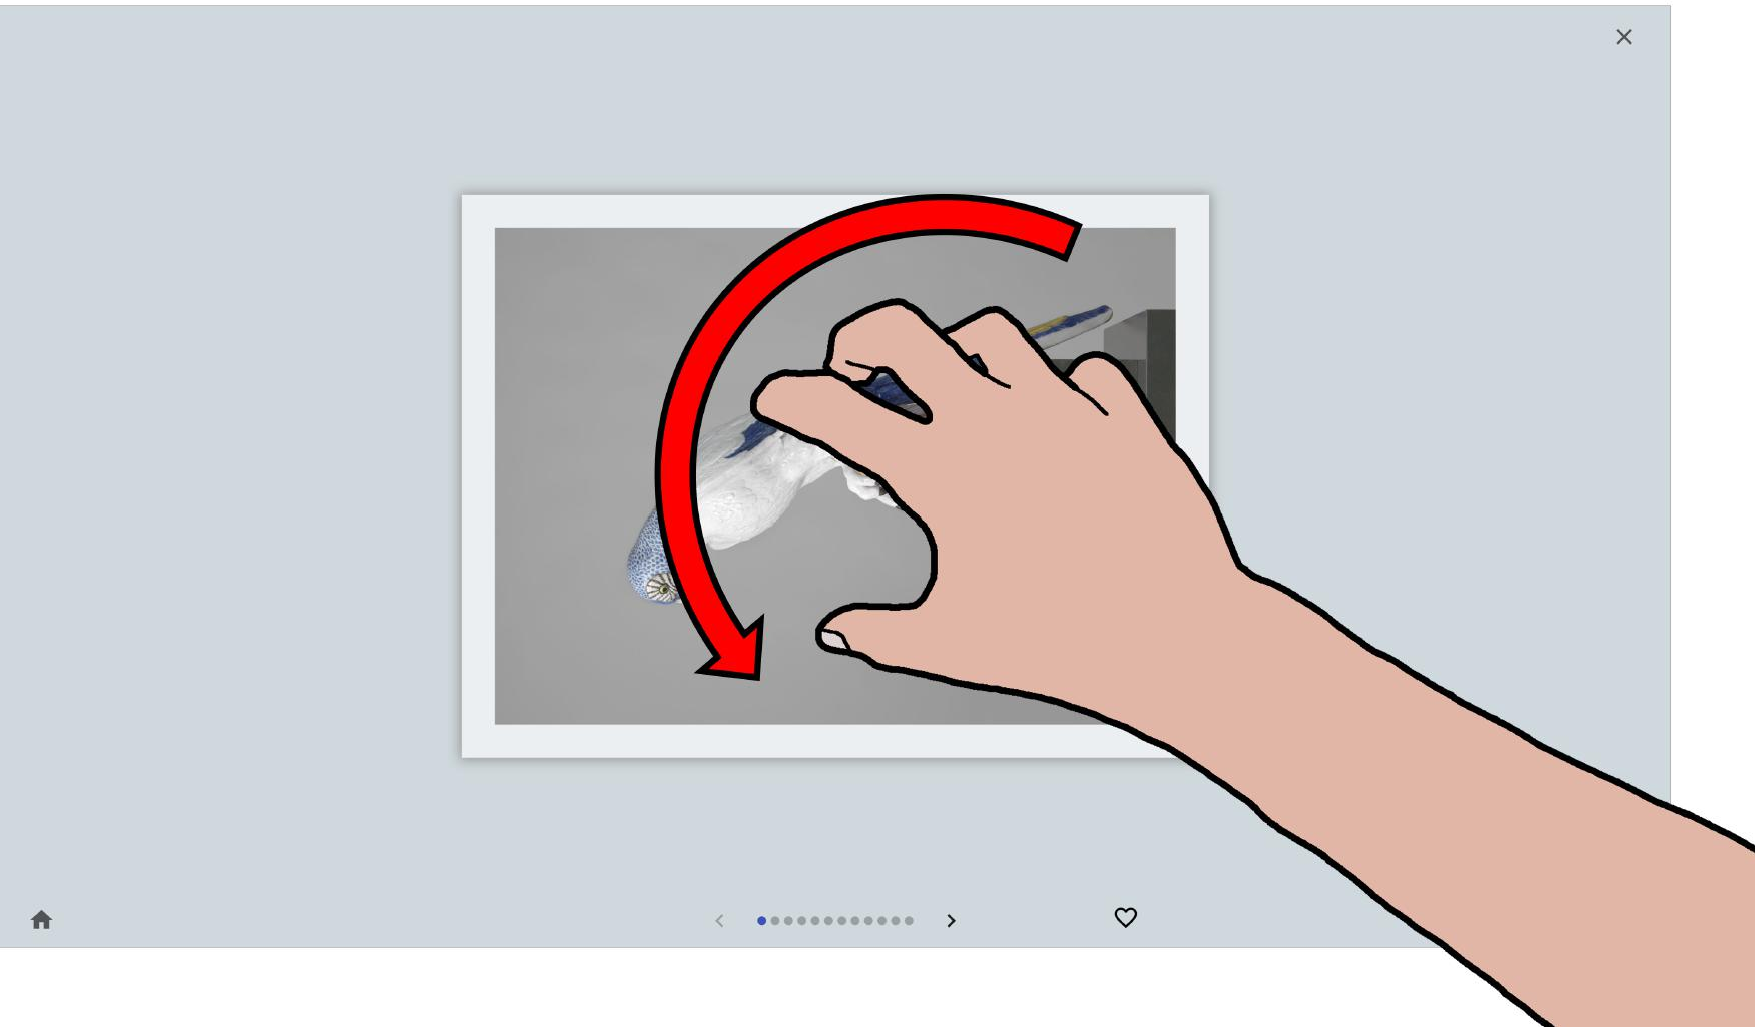
\includegraphics[width=.97\linewidth]{Figures/LUI/Gestures/rotate_counterclockwise.pdf}  
        \vspace{-6pt}
        \captionsetup{width=.9\linewidth}
        \caption{Rotate anti-clock.}
        \label{fig:lui:gestures:rotate-clock}
    \end{subfigure}
    \begin{subfigure}{.24\textwidth}
        \centering
        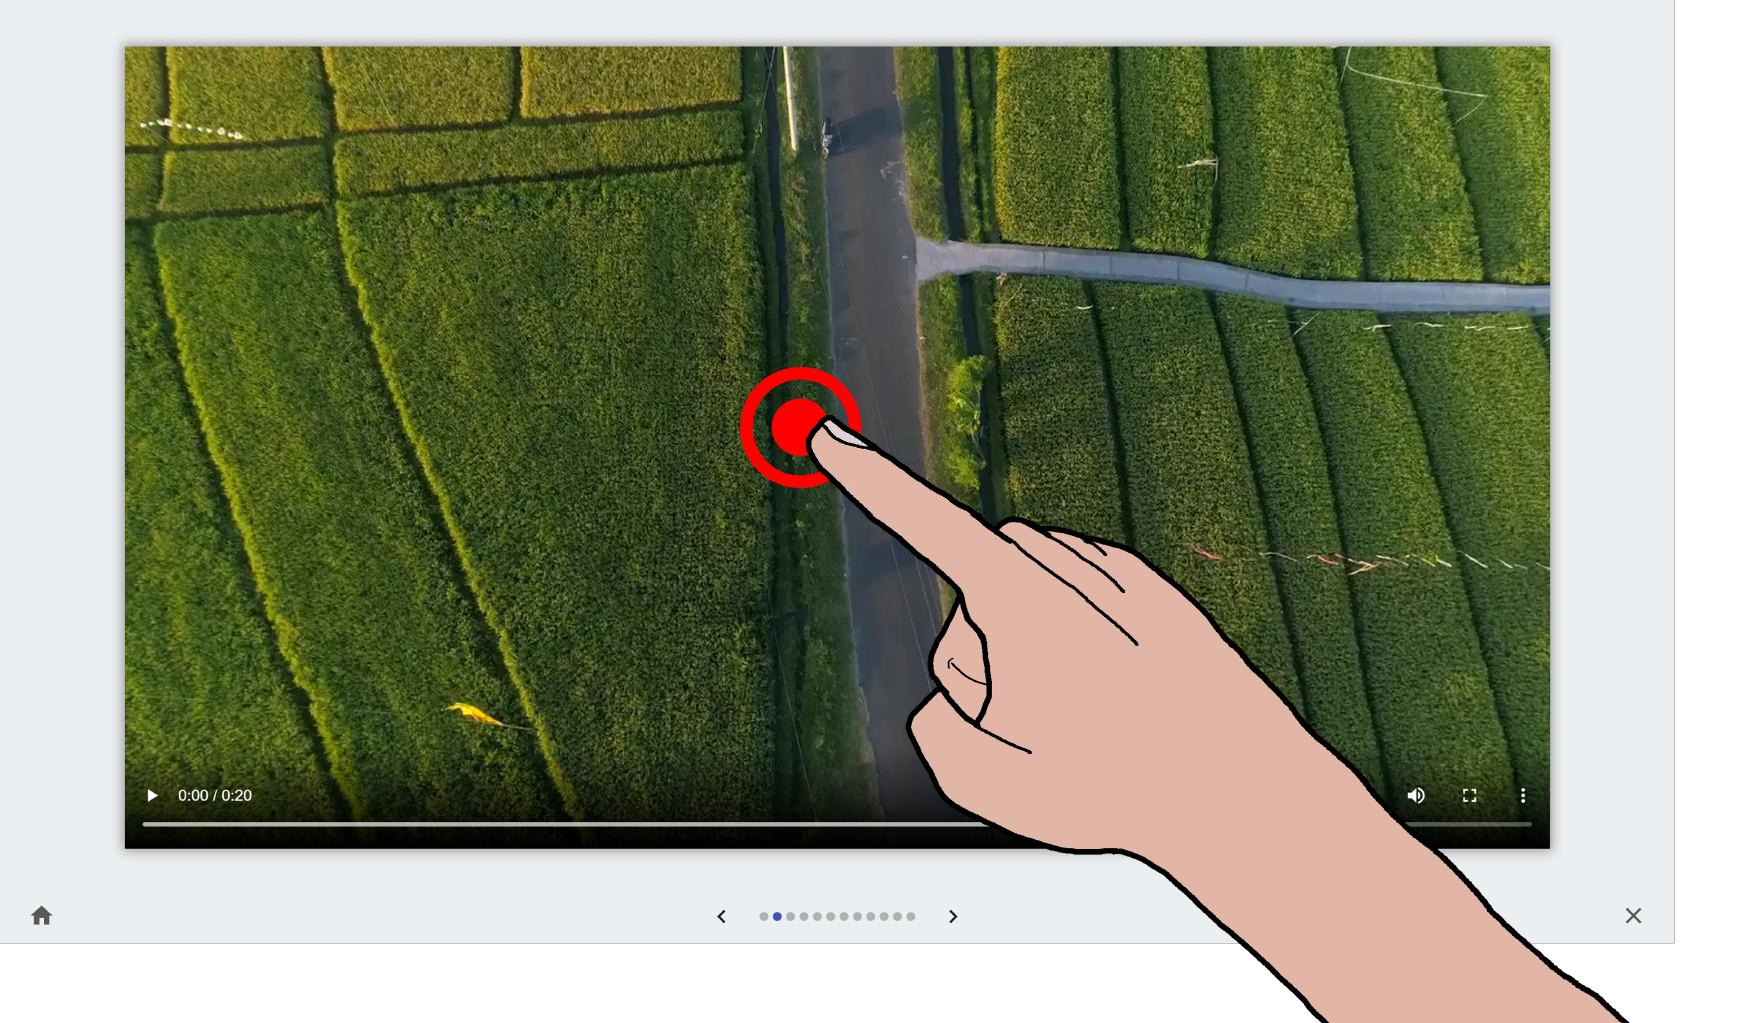
\includegraphics[width=.97\linewidth]{Figures/LUI/Gestures/tap-play.pdf} 
        \vspace{-6pt}
        \captionsetup{width=.9\linewidth}
        \caption{Play/pause.}
        \label{fig:lui:gestures:play-pause}
    \end{subfigure}
    \begin{subfigure}{.24\textwidth}
        \centering
        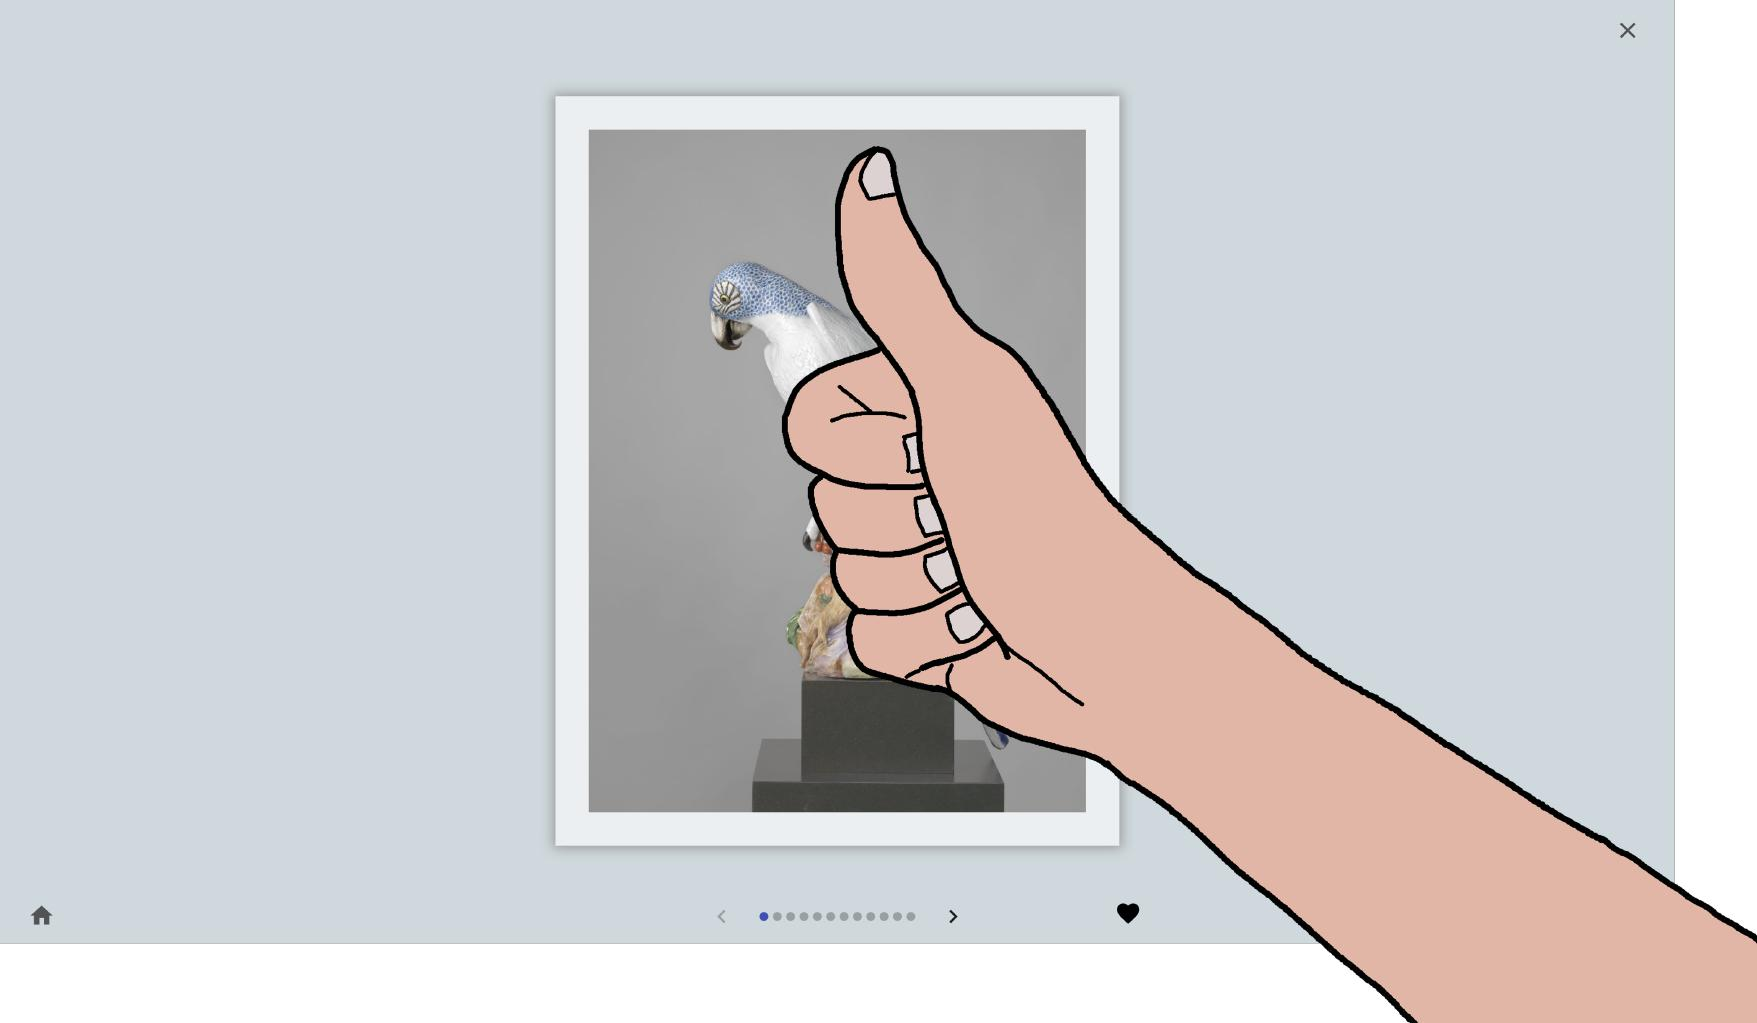
\includegraphics[width=.97\linewidth]{Figures/LUI/Gestures/thumb_up.pdf} 
        \vspace{-6pt}
        \captionsetup{width=.9\linewidth}
        \caption{Like.}
        \label{fig:lui:gestures:like}
    \end{subfigure}

    \begin{subfigure}{.24\textwidth}
        \centering
        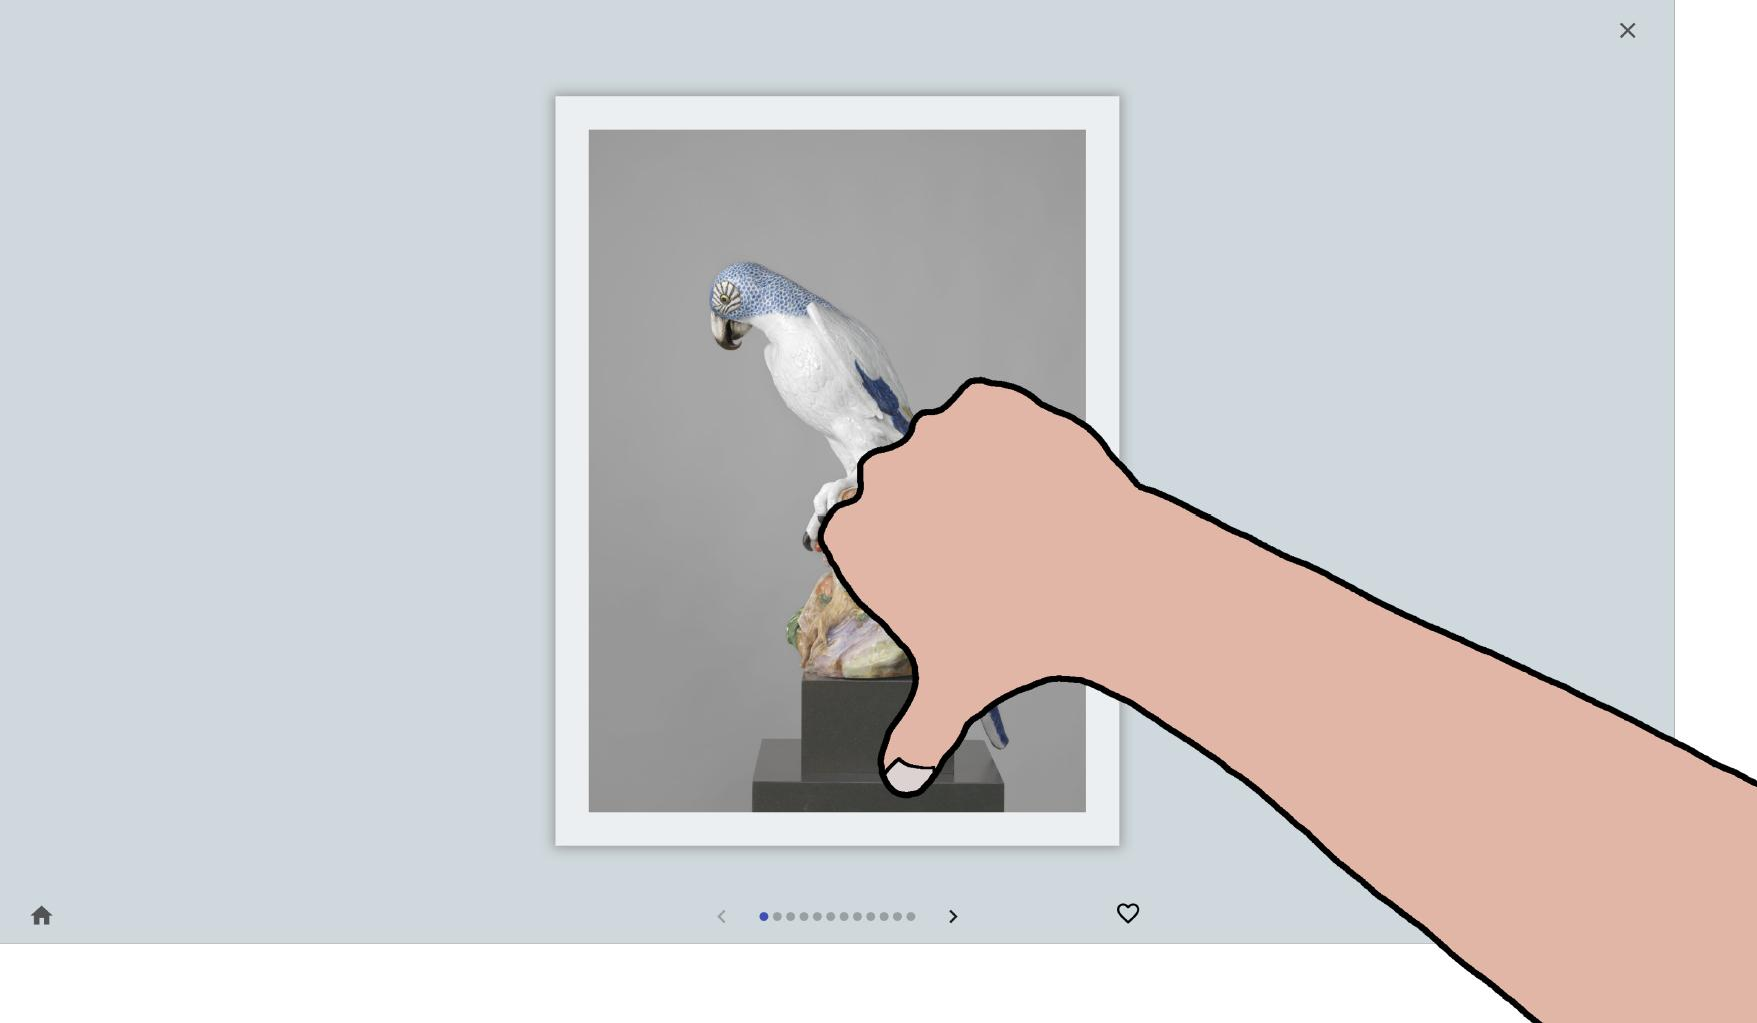
\includegraphics[width=.97\linewidth]{Figures/LUI/Gestures/thumb_down.pdf}  
        \vspace{-6pt}
        \captionsetup{width=.9\linewidth}
        \caption{Dislike.}
        \label{fig:lui:gestures:dislike}
    \end{subfigure}
    \begin{subfigure}{.24\textwidth}
        \centering
        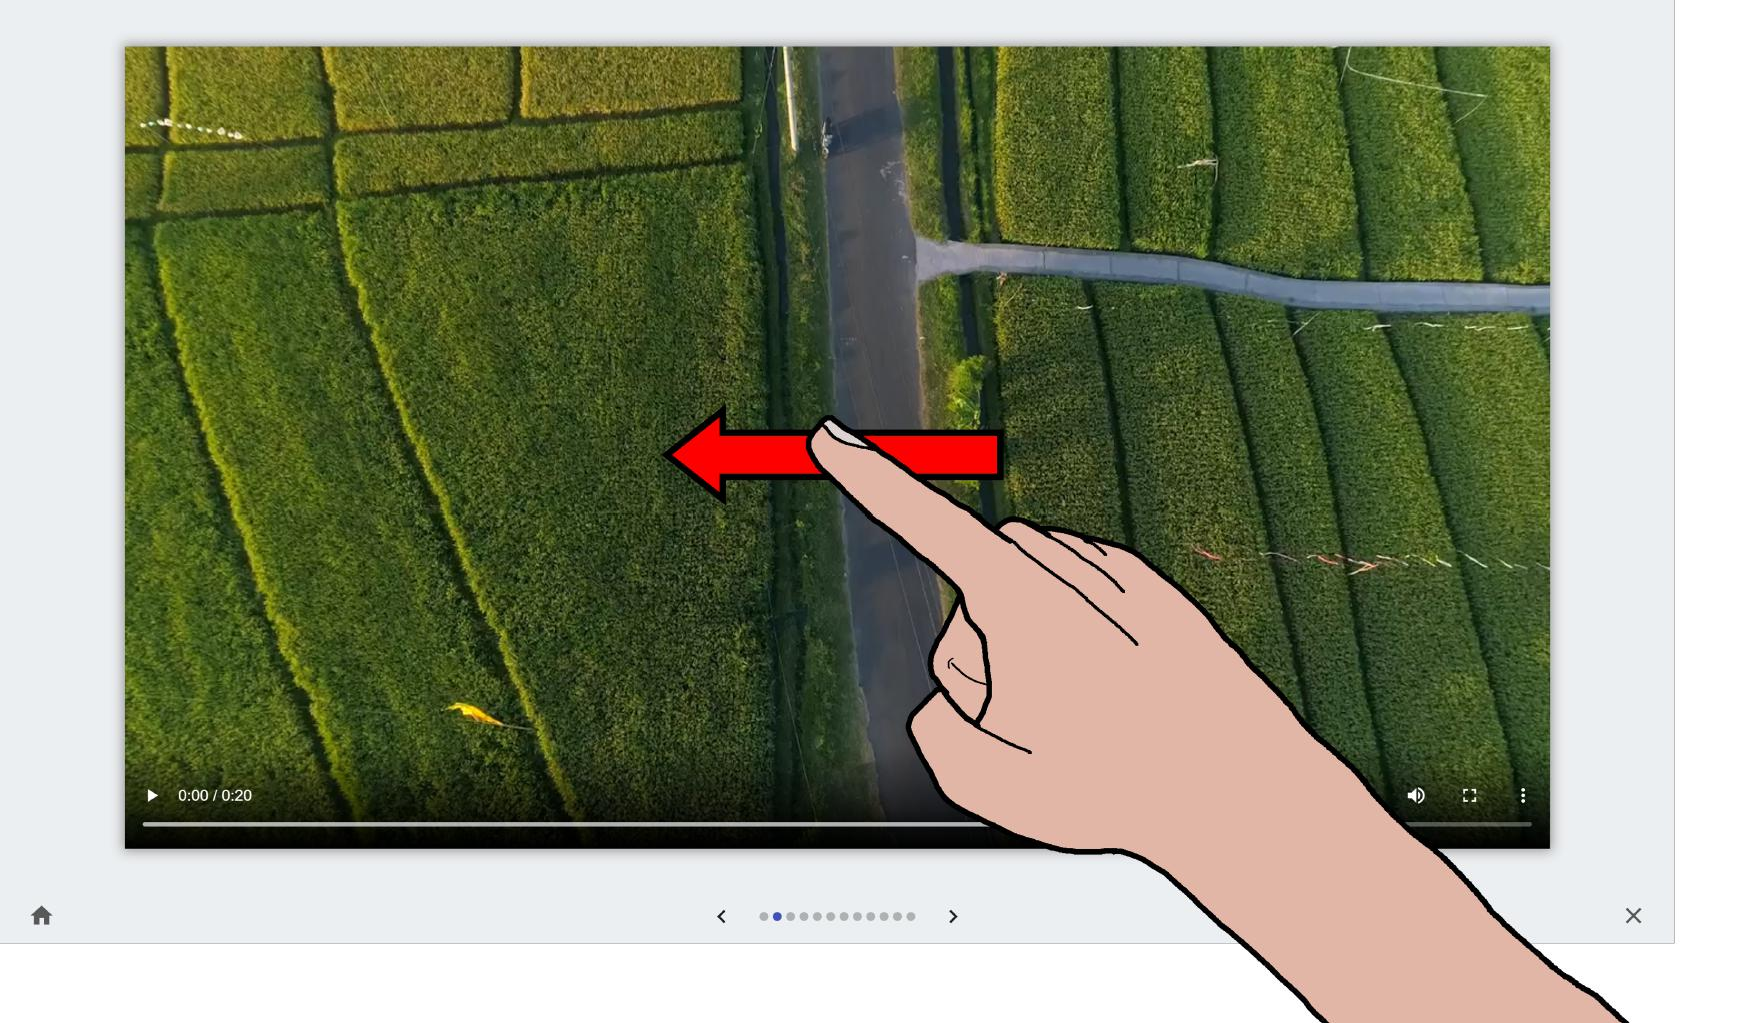
\includegraphics[width=.97\linewidth]{Figures/LUI/Gestures/swipe_left-seek.pdf}  
        \vspace{-6pt}
        \captionsetup{width=.9\linewidth}
        \caption{Fast forward.}
        \label{fig:lui:gestures:fast-forward}
    \end{subfigure}
    \begin{subfigure}{.24\textwidth}
        \centering
        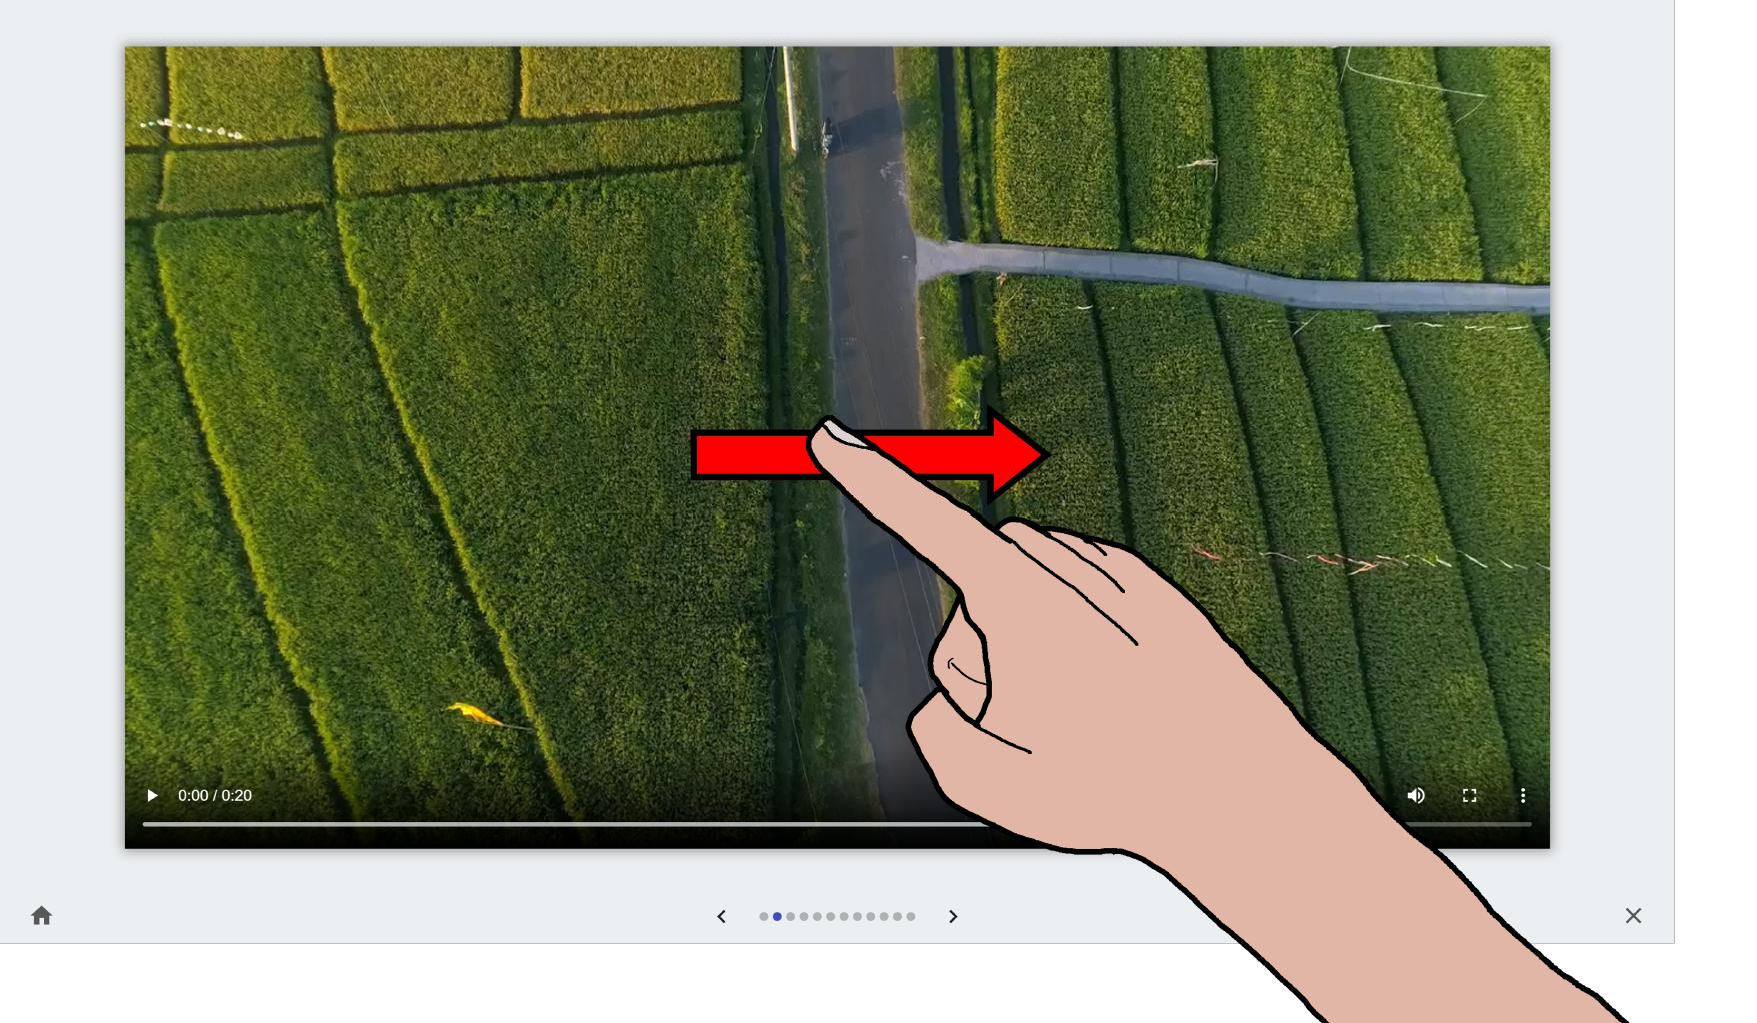
\includegraphics[width=.97\linewidth]{Figures/LUI/Gestures/swipe_right-seek.pdf}  
        \vspace{-6pt}
        \captionsetup{width=.9\linewidth}
        \caption{Rewind.}
        \label{fig:lui:gestures:rewind}
    \end{subfigure}
    \begin{subfigure}{.24\textwidth}
        \centering
        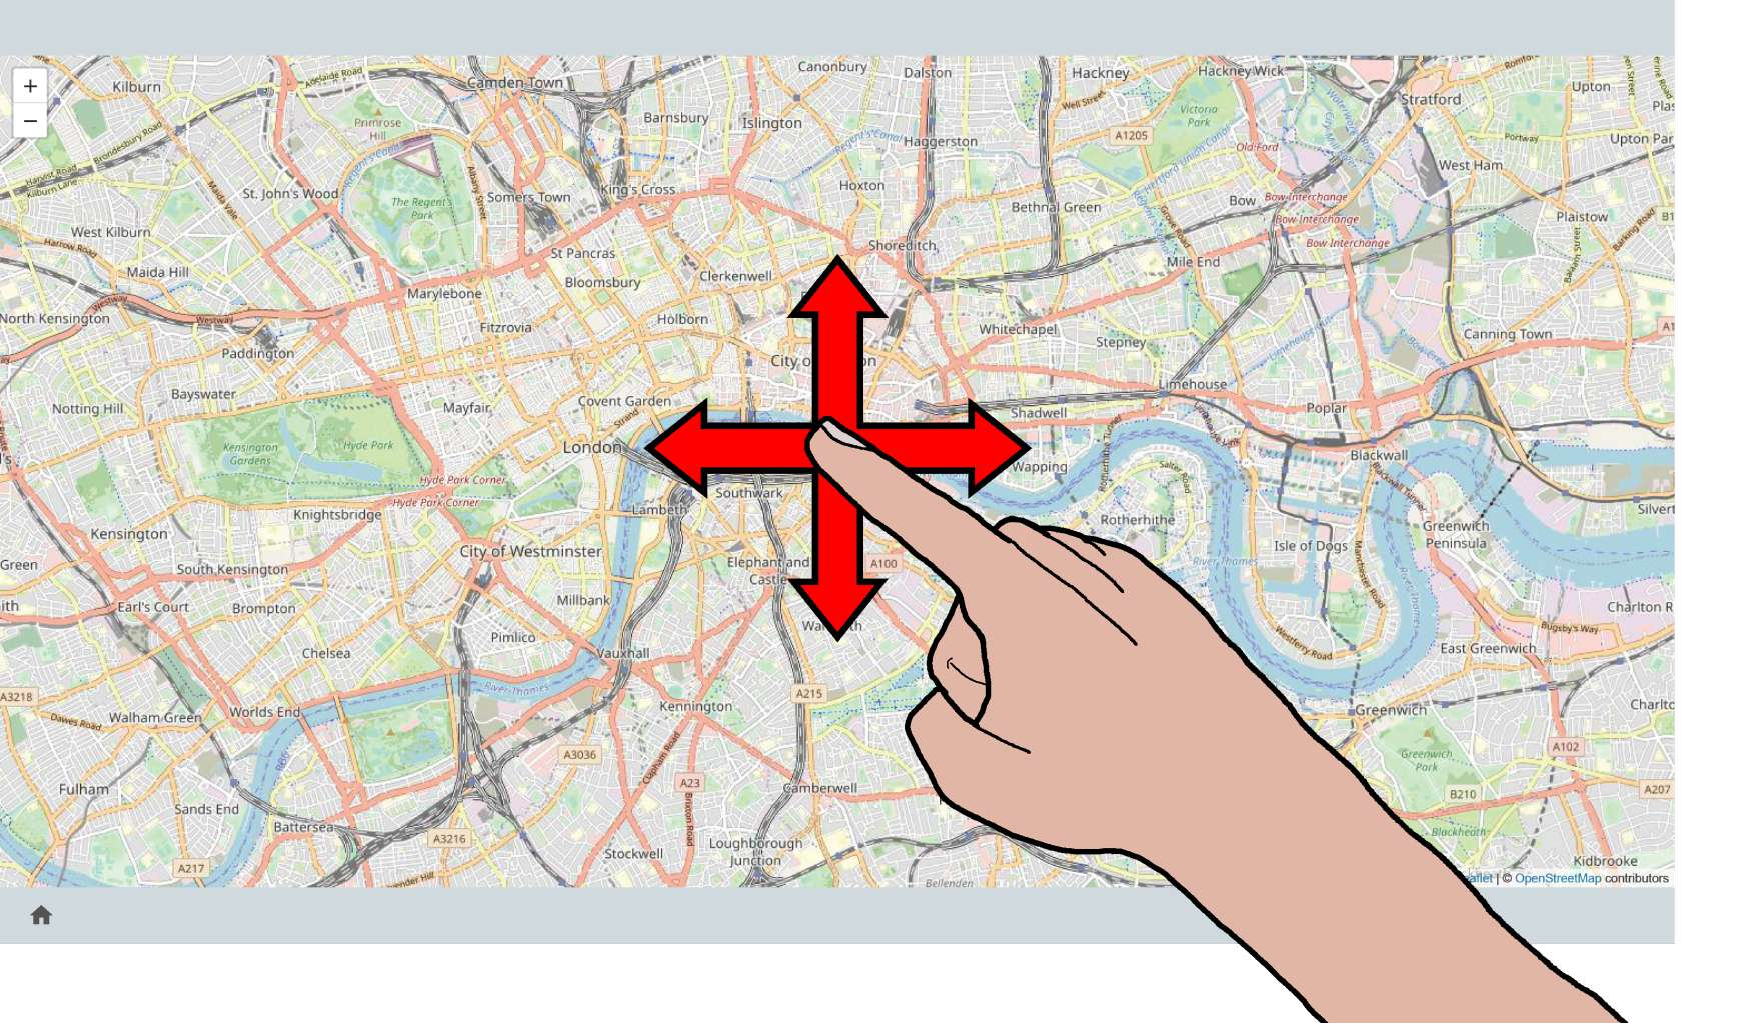
\includegraphics[width=.97\linewidth]{Figures/LUI/Gestures/pan.pdf}  
        \vspace{-6pt}
        \captionsetup{width=.9\linewidth}
        \caption{Pan.}
        \label{fig:lui:gestures:pan}
    \end{subfigure}
    % \vspace{-4pt}
    \caption{Illustrations of gestures mapped to each function in the \lui application.}
    \label{fig:lui:gestures}
%    \vspace{-6pt}
\end{figure}

\subsubsection{Gestures Selection} 
The \lui gesture set (\fig~\ref{fig:lui:gestures} and \tab~\ref{tab:lui:elicitation-to-recognition}) resulting from the contextual GES consists of gestures selected following four guidelines inspired by the literature~\cite{Morris:2010,Wobbrock:2005,Wobbrock:2009,Dingler:2018}:
\begin{enumerate}[noitemsep]
    \item Favor the most agreed gestures, as this usually results in a flatter learning curve and higher memorability~\cite{Wobbrock:2005,Wobbrock:2009,Dingler:2018}. For instance, we selected ``flick left'' instead of ``flick right'' for the ``next'' function, as the former was proposed by more participants.
    \item Prefer gestures that are less physically and mentally demanding to limit frustration and fatigue~\cite{Morris:2010}. For example, we favored one-handed over two-handed gestures.
    \item Map similar gestures to similar functions, independently of the media to increase memorability and flatten the learning curve~\cite{Dingler:2018}. For instance, we selected the same gesture for zooming in a photo/in a map and used symmetrical gestures for going to the previous/next item in a list.
    \item Map unique gestures to different functions occurring in the same context to avoid conflicts where one gesture would trigger multiple functions~\cite{Wobbrock:2005,Dingler:2018}.
\end{enumerate}
Together, these guidelines enabled us to build a conflict-free, highly guessable, and memorable gesture set that minimizes end users' mental and physical effort. The ``pan'' gesture was added later as part of the Maps application but was not part of the elicitation study.
%Due to the low consensus among participants, the ``enable subtitles'' and ``disable subtitles'' referents were not implemented in this version of \lui. 


% \noindent
% \begin{minipage}{\textwidth}
% \vspace{6pt}
%   \begin{minipage}[c]{0.30\textwidth}
%     \centering
%     \vspace{3pt}
%     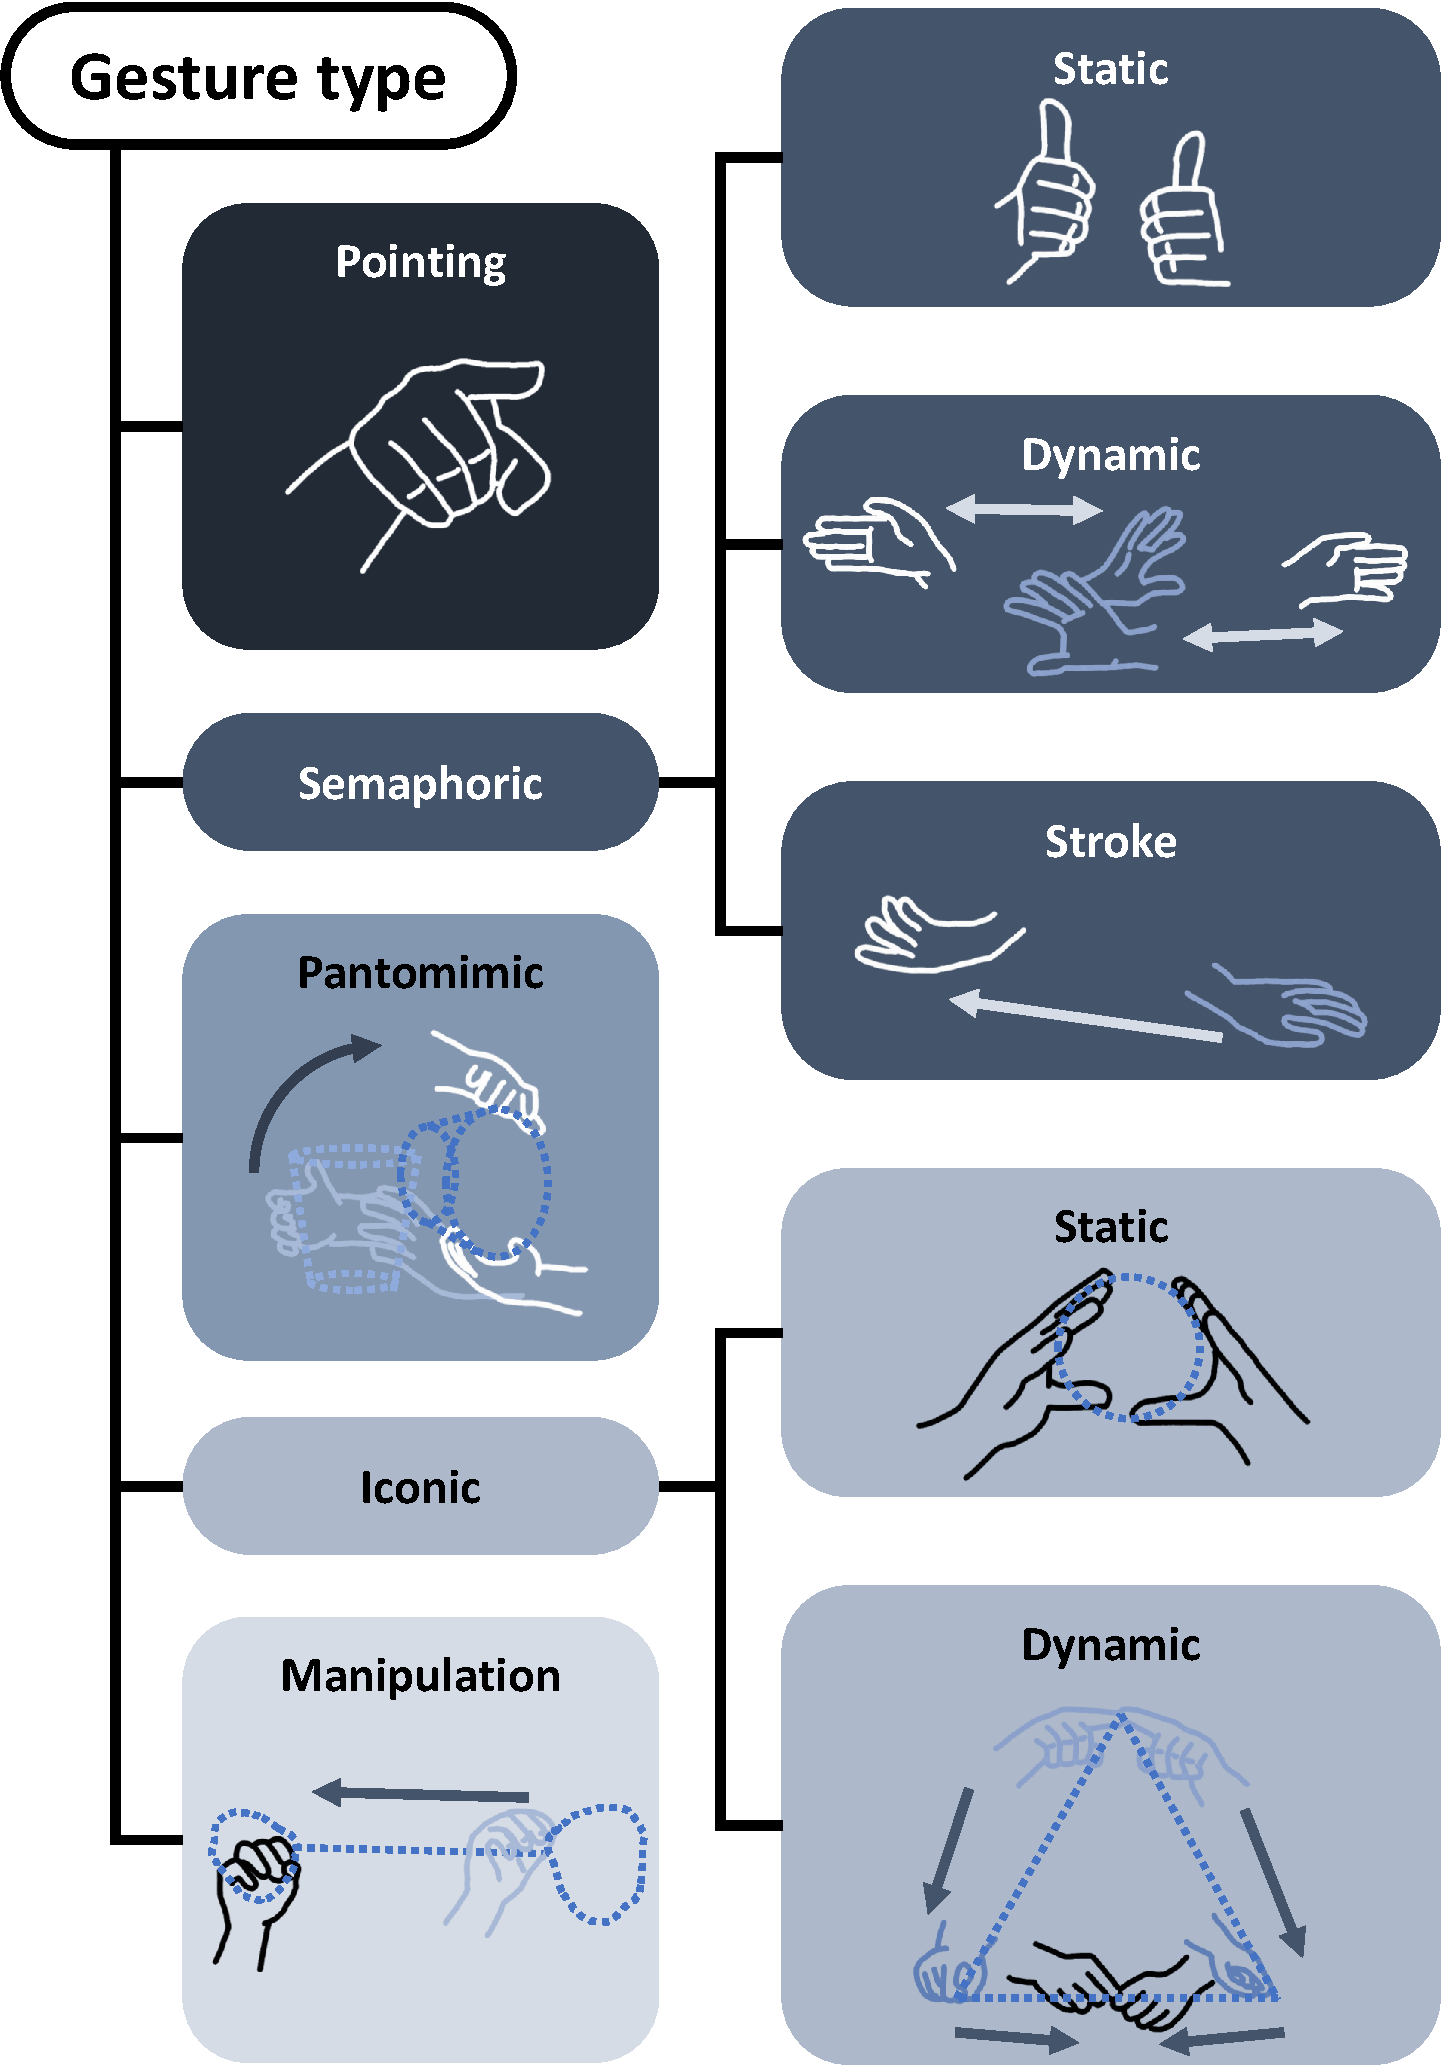
\includegraphics[width=\linewidth]{Figures/LUI/aigner.pdf}
%     \label{fig:lui:aigner-classification}
%     \vspace{-16pt}
%     \captionsetup{width=.99\linewidth}
%     \captionof{figure}{Aigner \etal's taxonomy~\cite{Aigner:2012}.}
%   \end{minipage}%
%   \begin{minipage}[c]{0.70\textwidth}
%     \centering
%     \footnotesize
%     \definecolor{semaphoric}{RGB}{68,84,106}
%     \definecolor{pointing}{RGB}{34,42,53}
%     \definecolor{manipulation}{RGB}{214,220,229}
%     \resizebox{\linewidth}{!}{
%     \renewcommand{\arraystretch}{1.1}
%     \begin{tabular}{lll|ll}%[noitemsep]
%     	\toprule
%     	\multicolumn{3}{c|}{\textbf{Elicitation}} & \multicolumn{2}{c}{\textbf{Recognition}}\\
%     	Action & Gesture & Category & Name & Type \\
%     	\midrule
%         Previous & Flick right & \cellcolor{semaphoric} \textcolor{white}{Stroke semaphoric} & Flick right & Dynamic \\
%         Next & Flick left & \cellcolor{semaphoric} \textcolor{white}{Stroke semaphoric} & Flick left & Dynamic \\
%         Enable fullscreen & Tap & \cellcolor{pointing} \textcolor{white}{Pointing} & Tap & Dynamic \\
%         Disable fullscreen & Flick up & \cellcolor{semaphoric} \textcolor{white}{Stroke semaphoric} & Flick up & Dynamic \\
%         Zoom in & Pinch out & \cellcolor{manipulation} Manipulation & Pinch & Static \\
%         Zoom out & Pinch in & \cellcolor{manipulation} Manipulation & Pinch & Static \\
%         Volume up & Swipe up & \cellcolor{manipulation} Manipulation & Point index & Static \\
%         Volume down & Swipe down & \cellcolor{manipulation} Manipulation & Point index & Static \\
%         Rotate clockwise &\shortstack[l]{Rotate a knob\\clockwise} & \cellcolor{manipulation} Manipulation & Grab & Static \\
%         Rotate anti-clockwise &\shortstack[l]{Rotate a knob\\anti-clockwise} & \cellcolor{manipulation} Manipulation & Grab & Static \\
%         Play & Tap & \cellcolor{semaphoric} \textcolor{white}{Stroke semaphoric} & Tap & Dynamic \\
%         Pause & Tap & \cellcolor{semaphoric} \textcolor{white}{Stroke semaphoric} & Tap & Dynamic \\
%         Like & Thumbs up & \cellcolor{semaphoric} \textcolor{white}{Static semaphoric} & Thumb & Static \\
%         Dislike & Thumbs down & \cellcolor{semaphoric} \textcolor{white}{Static semaphoric} & Thumb & Static \\
%         Fast-forward & Swipe left & \cellcolor{manipulation} Manipulation & Point index & Static \\
%         Rewind & Swipe right & \cellcolor{manipulation} Manipulation & Point index & Static \\
%         Pan & -- & -- & Point index & Static \\
%         \bottomrule
%     \end{tabular}
%     }
% %    \captionof{figure}{Aigner \etal' classification (left) used for classifying \lui gestures.}
%     \vspace{-8pt}
%     \captionsetup{width=.9\linewidth}
%   \captionof{table}{Classification of \lui gestures.}
%   \label{tab:lui:elicitation-to-recognition}
% \end{minipage}
% \vspace{-10pt}
% \end{minipage}


\begin{figure}[!b]
    \centering
    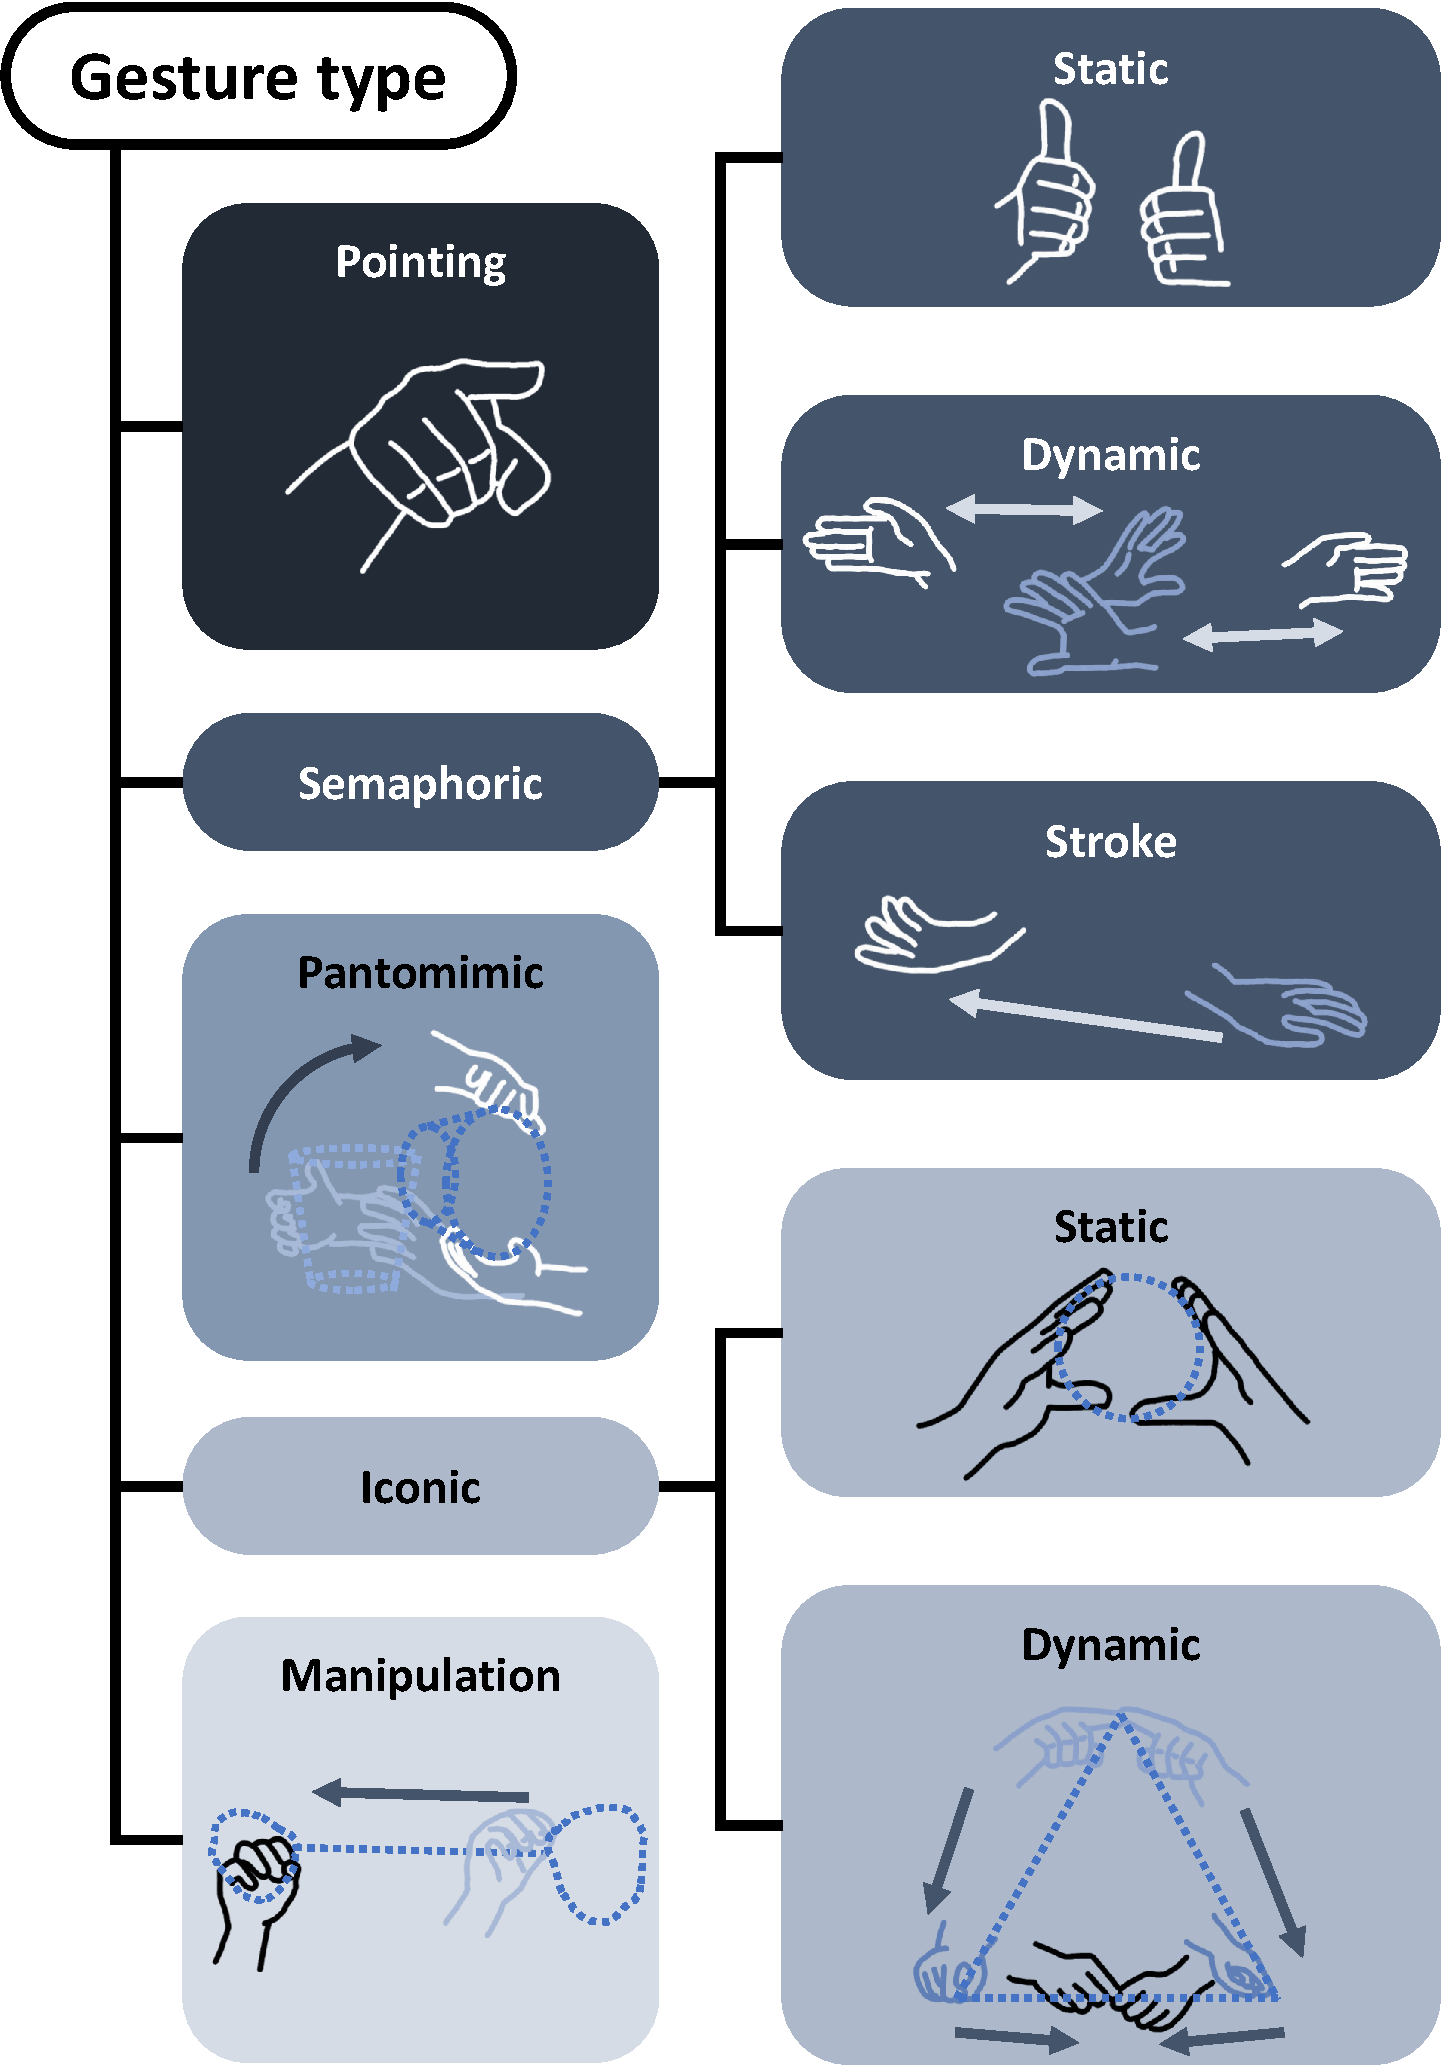
\includegraphics[width=.46\linewidth]{Figures/LUI/aigner.pdf}
    % \vspace{-4pt}
    \caption{Aigner \etal's taxonomy~\cite{Aigner:2012}.}
    \label{fig:lui:aigner-classification}
\end{figure}

\begin{table}[bt]
    \centering
    \footnotesize
    \renewcommand{\arraystretch}{1.1}
    \definecolor{semaphoric}{RGB}{68,84,106}
    \definecolor{pointing}{RGB}{34,42,53}
    \definecolor{manipulation}{RGB}{214,220,229}
    \begin{tabular}{lll|ll}%[noitemsep]
    	\toprule
    	\multicolumn{3}{c|}{\textbf{Elicitation}} & \multicolumn{2}{c}{\textbf{Recognition}}\\
    	Action & Gesture & Category & Name & Type \\
    	\midrule
        Previous & Flick right & \cellcolor{semaphoric} \textcolor{white}{Stroke semaphoric} & Flick right & Dynamic \\
        Next & Flick left & \cellcolor{semaphoric} \textcolor{white}{Stroke semaphoric} & Flick left & Dynamic \\
        Enable fullscreen & Tap & \cellcolor{pointing} \textcolor{white}{Pointing} & Tap & Dynamic \\
        Disable fullscreen & Flick up & \cellcolor{semaphoric} \textcolor{white}{Stroke semaphoric} & Flick up & Dynamic \\
        Zoom in & Pinch out & \cellcolor{manipulation} Manipulation & Pinch & Static \\
        Zoom out & Pinch in & \cellcolor{manipulation} Manipulation & Pinch & Static \\
        Volume up & Swipe up & \cellcolor{manipulation} Manipulation & Point index & Static \\
        Volume down & Swipe down & \cellcolor{manipulation} Manipulation & Point index & Static \\
        Rotate clockwise &\shortstack[l]{Rotate a knob\\clockwise} & \cellcolor{manipulation} Manipulation & Grab & Static \\
        Rotate anti-clockwise &\shortstack[l]{Rotate a knob\\anti-clockwise} & \cellcolor{manipulation} Manipulation & Grab & Static \\
        Play & Tap & \cellcolor{semaphoric} \textcolor{white}{Stroke semaphoric} & Tap & Dynamic \\
        Pause & Tap & \cellcolor{semaphoric} \textcolor{white}{Stroke semaphoric} & Tap & Dynamic \\
        Like & Thumbs up & \cellcolor{semaphoric} \textcolor{white}{Static semaphoric} & Thumb & Static \\
        Dislike & Thumbs down & \cellcolor{semaphoric} \textcolor{white}{Static semaphoric} & Thumb & Static \\
        Fast-forward & Swipe left & \cellcolor{manipulation} Manipulation & Point index & Static \\
        Rewind & Swipe right & \cellcolor{manipulation} Manipulation & Point index & Static \\
        Pan & -- & -- & Point index & Static \\
        \bottomrule
    \end{tabular}
    \vspace{-4pt}
    % \captionsetup{width=.9\linewidth}
    \caption{Classification of \lui gestures according to Aigner \etal's taxonomy~\cite{Aigner:2012}.}
    \label{tab:lui:elicitation-to-recognition}
\end{table}

\subsubsection{Gesture Classification} % classification of gestures towards gesture recognition
After designing a consistent and memorable gesture set, the next step was to determine how to efficiently recognize these gestures. As such, we first attempted to classify each gesture according to Aigner \etal's HCI-oriented gesture taxonomy~\cite{Aigner:2012}. While several multidisciplinary taxonomies exist in general for classifying gestures, including Kendon's taxonomy~\cite{Kendon:1988} and McNeil's taxonomy~\cite{McNeill:1995}, we rely on Aigner's classification as it identifies gesture classes suitable to the specific field of HCI by empirically validating 5,500 collected gestures on interactive functions without accompanying them with speech. Indeed, \cite{Ekman:1969} characterize human gestures according to three fundamental considerations, \ie origin, usage, and coding, and structure them into idiosyncratic, interactive, informative, and communicative classes.
Kendon~\cite{Kendon:1988} structures gestures along a continuum based on speech: gesticulation (beat, cohesives), language-like
(iconic), pantomimes, emblems (deictic), and sign language
(symbolic). McNeill~\cite{McNeill:1995} structures gestures into iconics, metaphorics, beats, cohesives, and deictics. 
By analyzing each gesture and its effect on the application, this step helped us identify the most appropriate configuration of \ql in the next section. \tab~\ref{tab:lui:elicitation-to-recognition} summarizes the results of our classification and details how each gesture should be recognized.


Eight of the 16 elicited gestures are classified in the \textit{manipulation} category, which are gestures for manipulating media objects in a short feedback loop. The gesture effect on the object is perceived in real-time while the user is performing it, with low latency~\cite{Aigner:2012} (\eg a response time of 0.1 sec to perceive interaction as direct manipulation and 1 sec to keep it seamless~\cite{Nielsen:1994}).
Other authors estimate the response time as follows: \cite{Chen:2017} situates the best compromise around 500 ms with a recognition rate above 90\%, while \cite{Annett:2014} report that end users perceive a response time of 50 ms for inking tasks on a touch-sensitive surface.
As an example of direct manipulation, the size of an image should change proportionally to the thumb-index distance while the user is performing a \textit{pinch in} or \textit{pinch out} gesture. For these gestures, the hand pose conveys the meaning of the gesture. They can thus be recognized by analyzing the user's hand pose in each frame in real-time. Six gestures are considered as \textit{stroke semaphoric} and two are considered as \textit{static semaphoric}. \textit{Semaphoric gestures} are hand poses and movements used to convey a specific meaning, often unrelated to the gesture. They can be further divided into three categories, including \textit{static} (if the meaning is entirely conveyed by the hand pose) and \textit{strokes} (which consist of single stroke hand motions)~\cite{Aigner:2012}. The \textit{stroke semaphoric} gestures could be recognized by analyzing the hand trajectory over time, while the \textit{static semaphoric} gestures could be recognized by analyzing the user's hand pose.
One gesture belongs to the \textit{pointing} category, \ie gestures which indicate objects and directions~\cite{Aigner:2012}. Indeed, to enable fullscreen, the \textit{tap} gesture acts as a selection method, as users first need to hover their finger above the selected item before performing the gesture. This gesture could be recognized similarly to the \textit{stroke semaphoric} gestures.
%\ie by analyzing the user's hand trajectory.


%--------------------------------------------------------------------------------%
\subsection{Software Architecture and Implementation} \label{sec:lui:development-method:implementation}
We used the \ql framework (Chapter~\ref{chap:quantumleap}) to implement gesture recognition into \lui, instead of developing a pipeline from scratch. 
Using the \ql API, gestures were assigned effects on the UI to be triggered each time they were recognized. For instance, the \textit{pinch} static gesture rotates a picture depending on the angle of the user's hand, and the \textit{tap} dynamic gesture opens an application, displays content in fullscreen, or plays/pauses a video, depending on the context. 
%
The use of \ql has multiple benefits. For instance, changes to the gesture set or updates to the gesture recognition pipeline do not require any modification to the \lui source code. In addition, the implementation of gesture recognition into \lui was extremely quick, as we could just select the most appropriate modules among those already supported by the framework. 
%
In the rest of this section, we motivate our choice of modules by conducting a comparative testing of static and dynamic gesture recognizers (see \cite{Magrofuoco:2021} for a survey in 2D) and discussing the use of a sliding window for gesture segmentation. 

\begin{table*}[b]
    \resizebox{\linewidth}{!}{
	\renewcommand{\arraystretch}{1.1}
	\centering
	\captionsetup{justification=centering}
	\begin{tabular}{lr|rrrrrr|rr|r}
	    \toprule
        \multicolumn{2}{c|}{\textbf{Recognizer}} & \multicolumn{6}{c|}{\textbf{Gesture class}} & \multicolumn{2}{c|}{\textbf{Global accuracy}} & \multirow{2}{*}{\textbf{Time}} \\
		 Name & $A$ & Flat & Point & Pinch & Grab & Thumb & Idle & Mean & SD & \\
		\midrule
        \$P\textsuperscript{3}+ & 6 & 99.7\% & 100.0\% & 100.0\% & 100.0\% & 100.0\% & 100.0\% & \cellcolor{highlightcolor} 99.9\% & 0.1\% & 0.15ms \\
        \$P\textsuperscript{3}+ & 16 & 100.0\% & 99.9\% & 99.7\% & 100.0\% & 100.0\% & 100.0\% & \cellcolor{highlightcolor} 99.9\% & 0.1\% & 0.46ms \\
        GPSDa & 6 & 99.6\% & 99.0\% & 98.3\% & 99.9\% & 98.2\% & 100.0\% & \cellcolor{highlightcolor} 99.2\% & 0.8\% & 0.04ms \\
        GPSDa & 16 & 99.6\% & 99.8\% & 99.4\% & 100.0\% & 99.5\% & 100.0\% & \cellcolor{highlightcolor} 99.7\% & 0.3\% & 0.22ms \\
        \bottomrule
	\end{tabular}
	}
	\vspace{-4pt}
	\caption{Recognition rate of each static recognizer, for $T{=}128$. Accuracy higher than 98\% is highlighted in blue.}
	\label{tbl:results-static}
	% \vspace{-5pt}
\end{table*}

\subsubsection{Static Gestures}
Two static gesture recognizers were tested on a custom gesture set containing six types of poses (grab, pinch, point index, flat hand, thumb, and rest) acquired from one participant. Each pose was performed in various orientations and scales, resulting in more than 1000 templates per class. The study is within-factors with three independent variables: 
\begin{itemize}
    \item \custominlinehighlight{Recognizer}: nominal variable with two conditions, representing the static recognizers tested (Appendix~\ref{app:quantumleap-modules:static-recognizers}): GPSDa, a custom recognizer with  $\alpha{=}0.65$) and \$P\textsuperscript{3}+, a implementation of Vatavu's \$P+~\cite{Vatavu:2017a} that supports 3D gestures.
    \item \custominlinehighlight{Number of Joints}: numerical variable with two conditions, representing the number of joints used by the recognizers: $A{\in}\{6,16\}$.
    \item \custominlinehighlight{Number of Templates}: numerical variable with eight conditions, representing the number of gesture templates used to train the recognizers: $\splitatcommas{T{\in}\{1,2,4,8,16,32,64,128\}}$.
\end{itemize}
The testing was conducted using the \ql testing tool (Chapter~\ref{chap:quantumleap-testing}) following a train-test-split (TTS) procedure with 1000 repetitions in a user-dependent and single-dataset scenario (see \tab~\ref{tab:quantumleap-testing:testing-procedures} for a detailed description of the procedure).

% The testing procedure is as follows: for each recognizer, each value of $A$ and $T$, and each gesture class, we repeat 1000 times: (1) select a random testing template from the gesture set; (2) train the recognizer using $T$ randomly selected templates, produced by the same user as the testing template (user-dependent testing); and (3) recognize the testing template. 

This experiment shows that GPSDa exhibits a different behavior than \$P\textsuperscript{3}+ (\tab~\ref{tbl:results-static}): GPSDa performs better with a larger number of joints, while the opposite occurs for \$P\textsuperscript{3}+. GPSDa performs better than \$P\textsuperscript{3}+ with a small number of templates (\eg with 4 templates, GPSDa ($A{=}16$) reaches $91.0\%$ accuracy against $87.1\%$ for \$P\textsuperscript{3}+ ($A{=}6$)), but \$P\textsuperscript{3}+ starts performing better as the number of templates increases. Both recognizers achieved ${>}99\%$ accuracy with 128 training templates. Despite \$P\textsuperscript{3}+ being very slightly better in the benchmark, GPSDa was selected for the \lui application as its rotation invariance gives it an edge in real-world situations (\eg when the user's hand is rotated relative to the training samples).

\subsubsection{Dynamic Gestures}
Similarly to the static gesture recognizers, eight dynamic gesture recognizers were tested on the \lui gesture set to determine the best-suited recognizer. The gesture set contains four types of pre-segmented dynamic gestures, \ie \textit{flick left}, \textit{flick right}, \textit{flick up}, and \textit{tap}, acquired from four participants. Gestures were performed four times by each participant, giving 16 templates per class. The study is within-factors with three independent variables: 
\begin{enumerate}
    \item \custominlinehighlight{Recognizer}: nominal variable with five conditions, representing the dynamic recognizers tested:  3 cent~\cite{Caputo:2017}, \$P\textsuperscript{3} (adapted from \$P~\cite{Vatavu:2012}), \$P\textsuperscript{3}+ (adapted from \$P+~\cite{Vatavu:2017a}), \$Q\textsuperscript{3} (adapted from \$Q~\cite{Vatavu:2018}), and Jackknife~\cite{Taranta:2017}. The recognizers are detailed in Appendix~\ref{app:quantumleap-modules:dynamic-recognizers}.
    \item \custominlinehighlight{Number of Joints}: numerical variable with three conditions, representing the number of joints taken into account by the recognizers: $A{\in}\{1, 6, 16\}$.
    \item \custominlinehighlight{Number of Templates}: numerical variable with four conditions, representing the number of gesture templates used to train the recognizers: $\splitatcommas{T{\in}\{1,2,4,8\}}$.
\end{enumerate}
The testing procedure was similar to the one used for static recognizers, but each gesture template was resampled to 16 points.
%The testing procedure is similar to the one used for static recognizers: for each recognizer, for each value of $A$ and $T$, and each gesture class, we repeat the three following steps 1000 times: (1) select a random testing template from the gesture set; (2) train the recognizer using $T$ randomly selected templates produced by different users than the testing template (user-independent testing); and (3) attempt to recognize the testing template. Each template was first resampled to 16 points.

Because the dataset includes only four simple gestures, the recognition rates are very high for most recognizers even with very few training templates (\tab~\ref{tbl:results-dynamic}, $T{=}8$). Jackknife already reaches $100\%$ with one training template and accuracy for all recognizers generally increases with the number of training templates. %Table \ref{tbl:results-dynamic} summarizes recognition rates for $T{=}8$.
Jackknife ($A{=}1$) was selected as the dynamic recognizer for \lui, as it maximizes accuracy and minimizes the execution time on this dataset.

\begin{table*}[t]
    \resizebox{\linewidth}{!}{
	\renewcommand{\arraystretch}{1.1}
	\captionsetup{justification=centering}
	\resizebox{\linewidth}{!}{
	\begin{tabular}{lr|rrrr|rr|r}
	    \toprule
        \multicolumn{2}{c|}{\textbf{Recognizer}} & \multicolumn{4}{c|}{\textbf{Gesture class}} & \multicolumn{2}{c|}{\textbf{Global accuracy}} & \multirow{2}{*}{\textbf{Time}} \\
		Name & $A$ & Flick up & Flick left & Flick right & Tap & Mean & SD & \\
		\midrule
        3\textcent & 1 &  100.0\% & 97.2\% & 100.0\% & 100.0\% & \cellcolor{highlightcolor} 99.3\% & 1.4\% & 0.78ms \\
        \$P\textsuperscript{3} & 1 &  100.0\% & 67.7\% & 70.1\% & 100.0\% & 84.5\% & 18.0\% & 0.33ms \\
        \$P\textsuperscript{3} & 6 &  94.3\% & 91.5\% & 80.3\% & 99.9\% & 91.5\% & 8.2\% & 0.38ms \\
        \$P\textsuperscript{3} & 16 &  91.9\% & 99.9\% & 90.8\% & 100.0\% & 95.7\% & 5.0\% & 0.28ms \\
        \$P\textsuperscript{3}+ & 1 &  100.0\% & 58.9\% & 53.5\% & 100.0\% & 78.1\% & 25.4\% & 0.05ms \\
        \$P\textsuperscript{3}+ & 6 &  99.9\% & 85.8\% & 78.1\% & 100.0\% & 91.0\% & 10.9\% & 0.06ms\\
        \$P\textsuperscript{3}+ & 16 &  100.0\% & 94.2\% & 83.0\% & 100.0\% & 94.3\% & 8.0\% & 0.10ms\\
        \$Q\textsuperscript{3} & 1 &  100.0\% & 65.9\% & 36.1\% & 100.0\% & 75.5\% & 30.8\% & 0.91ms \\
        \$Q\textsuperscript{3} & 6 &  100.0\% & 82.1\% & 71.6\% & 100.0\% & 88.4\% & 14.0\% & 1.03ms \\
        \$Q\textsuperscript{3} & 16 &  99.2\% & 90.8\% & 75.2\% & 100.0\% & 91.3\% & 11.5\% & 0.97ms \\
        Jackknife & 1 &  100.0\% & 100.0\% & 100.0\% & 100.0\% & \cellcolor{highlightcolor} 100.0\% & 0.0\% & 0.04ms \\
        Jackknife & 6 &  100.0\% & 100.0\% & 100.0\% & 100.0\% & \cellcolor{highlightcolor} 100.0\% & 0.0\% & 0.10ms \\
        Jackknife & 16 &  100.0\% & 100.0\% & 100.0\% & 100.0\% & \cellcolor{highlightcolor} 100.0\% & 0.0\% & 0.19ms \\
        \bottomrule
	\end{tabular}
	}
	}
	\vspace{-4pt}
	\caption{Recognition rate of each dynamic recognizer, for $T{=}8$. Recognizers with a global accuracy higher than 98\% are highlighted in blue.}
	\vspace{-10pt}
	\label{tbl:results-dynamic}
\end{table*}

\subsubsection{Gesture Segmentation}
A simple sliding window was selected for gesture segmentation. Sliding windows are easy to implement, fast to execute, require no specific user input, and have been combined with recognizers such as Jackknife~\cite{Taranta:2017} and 3\textcent~\cite{Caputo:2019}. However, they are sensitive to parasitic gestures, which may hinder the user experience. To address this issue, it was combined with two other techniques: (1) a motion rejection threshold to reject small hand motions such as hand tremors, and (2) a rejection threshold based on the score returned by the recognizers, to reject poorly performed gestures. In the future, more advanced segmentation techniques \cite{Kratz:2015,Chen:2016,Taranta:2021} could be incorporated into a new module for \ql without requiring any code modification to \lui.

\subsubsection{Final Configuration}
\fig~\ref{fig:lui:quantumleap} shows the final \ql pipeline configuration for the \lui application. The Window segmenter and Jackknife recognizer identify users' hand gestures from the continuous flow of data. The Basic analyzer and GPSDa recognizer identify static hand gestures and allow the manipulation of images, videos, and documents with continuous feedback.

\begin{figure}[!b]
    \centering
    % \vspace{-6pt}
    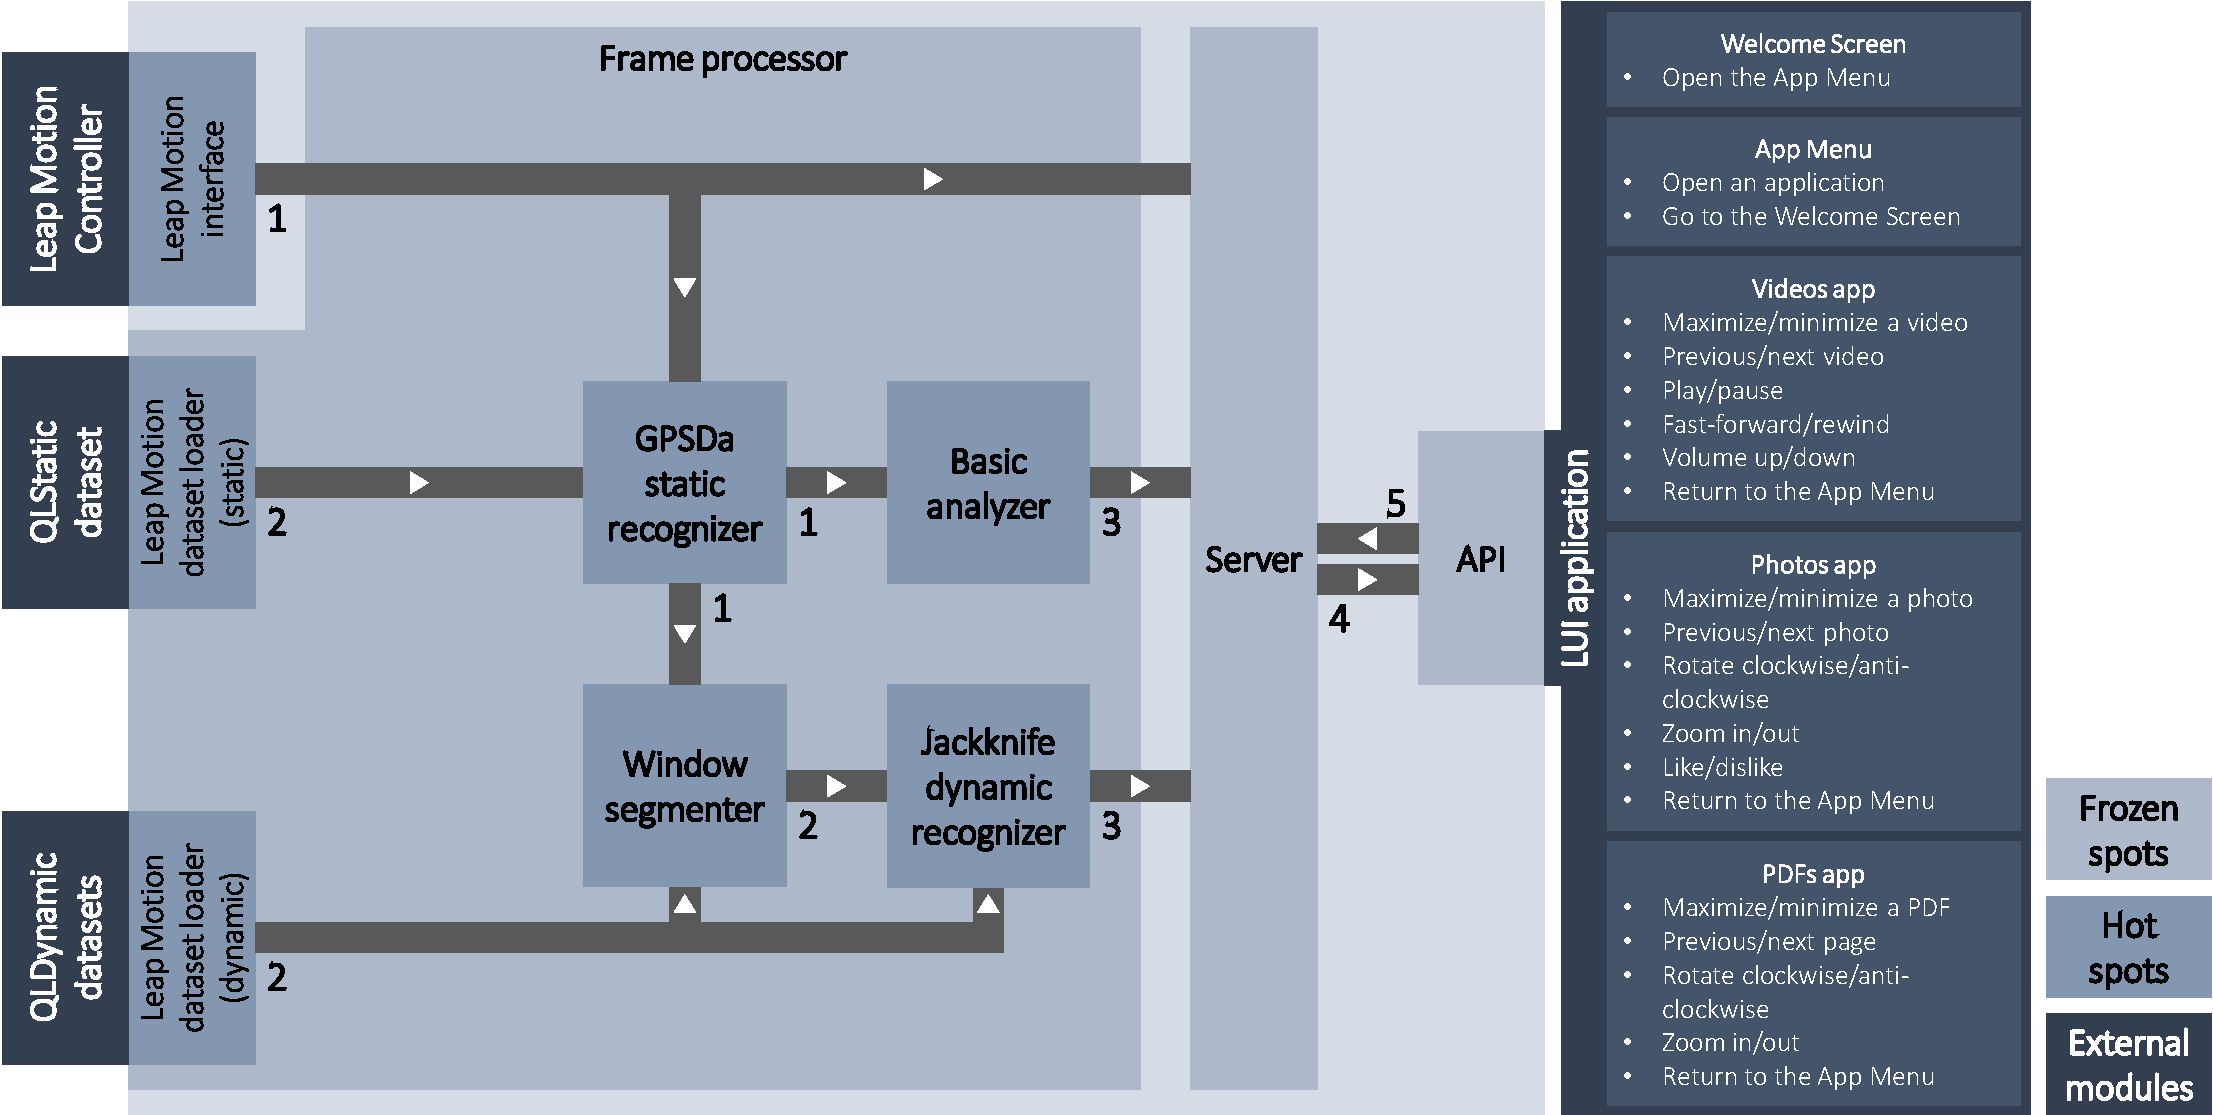
\includegraphics[width=\linewidth]{Figures/LUI/Architecture/quantumleap-lui.pdf}
    \vspace{-16pt}
    \caption{Instantiation of the \ql framework for \lui.}
    \label{fig:lui:quantumleap}
    % \vspace{-16pt}
\end{figure}

In addition to simplifying future modifications to the \lui gesture recognition pipeline, the use of \ql reduced the size of its source code by around 1280 lines of code (LOCs), distributed as follows: 
\begin{itemize}[noitemsep]
    \item 101 LOCs to connect to the LMC and extract data in the correct format.
    \item 110 LOCs to load the dynamic gesture dataset.
    \item 63 LOCs to load the static gesture dataset.
    \item 143 LOCs for the GPSDa static recognizer.
    \item 60 LOCs for the analyzer.
    \item 78 LOCs for the window segmenter.
    \item 725 LOCs for the JackKnife dynamic gesture recognizer.
\end{itemize}
If we factor out the time required to conceive, design, and develop an adequate pipeline for gesture recognition from scratch, and to integrate it into a working environment, the benefits of \ql in terms of time-saving become more obvious than in terms of LOCs saving.

% %--------------------------------------------------------------------------------%
% \subsection{Gesture Recognition Pipeline}


%================================================================================%
\section{Evaluation} \label{sec:lui:evaluation}
This section reports the results of an experiment performed on the third \lui version, according to a procedure inspired by~\cite{Vogiatzidakis:2022}.

%--------------------------------------------------------------------------------%
\subsection{Experiment Protocol} \label{sec:lui:evaluation:protocol}
\subsubsection{Environment}
The experiment involved multiple devices, including a large TV screen for displaying the \lui application and tutorial videos (\fig~\ref{fig:lui:evaluation-apparatus}), an LMC for capturing the participants' gestures, and a laptop for running the \lui application and controlling the experiment with a custom software. A camera was positioned to record both the participants' hands and the TV screen. The \lui application was configured to record the logs of the gestures recognized by the system.
Participants were installed at a desk and faced a large screen situated around two meters on the opposite side of the desk. The LMC was positioned in front of them.

\begin{figure}[htb]
    \centering
    \begin{subfigure}{.495\textwidth}
        \centering
        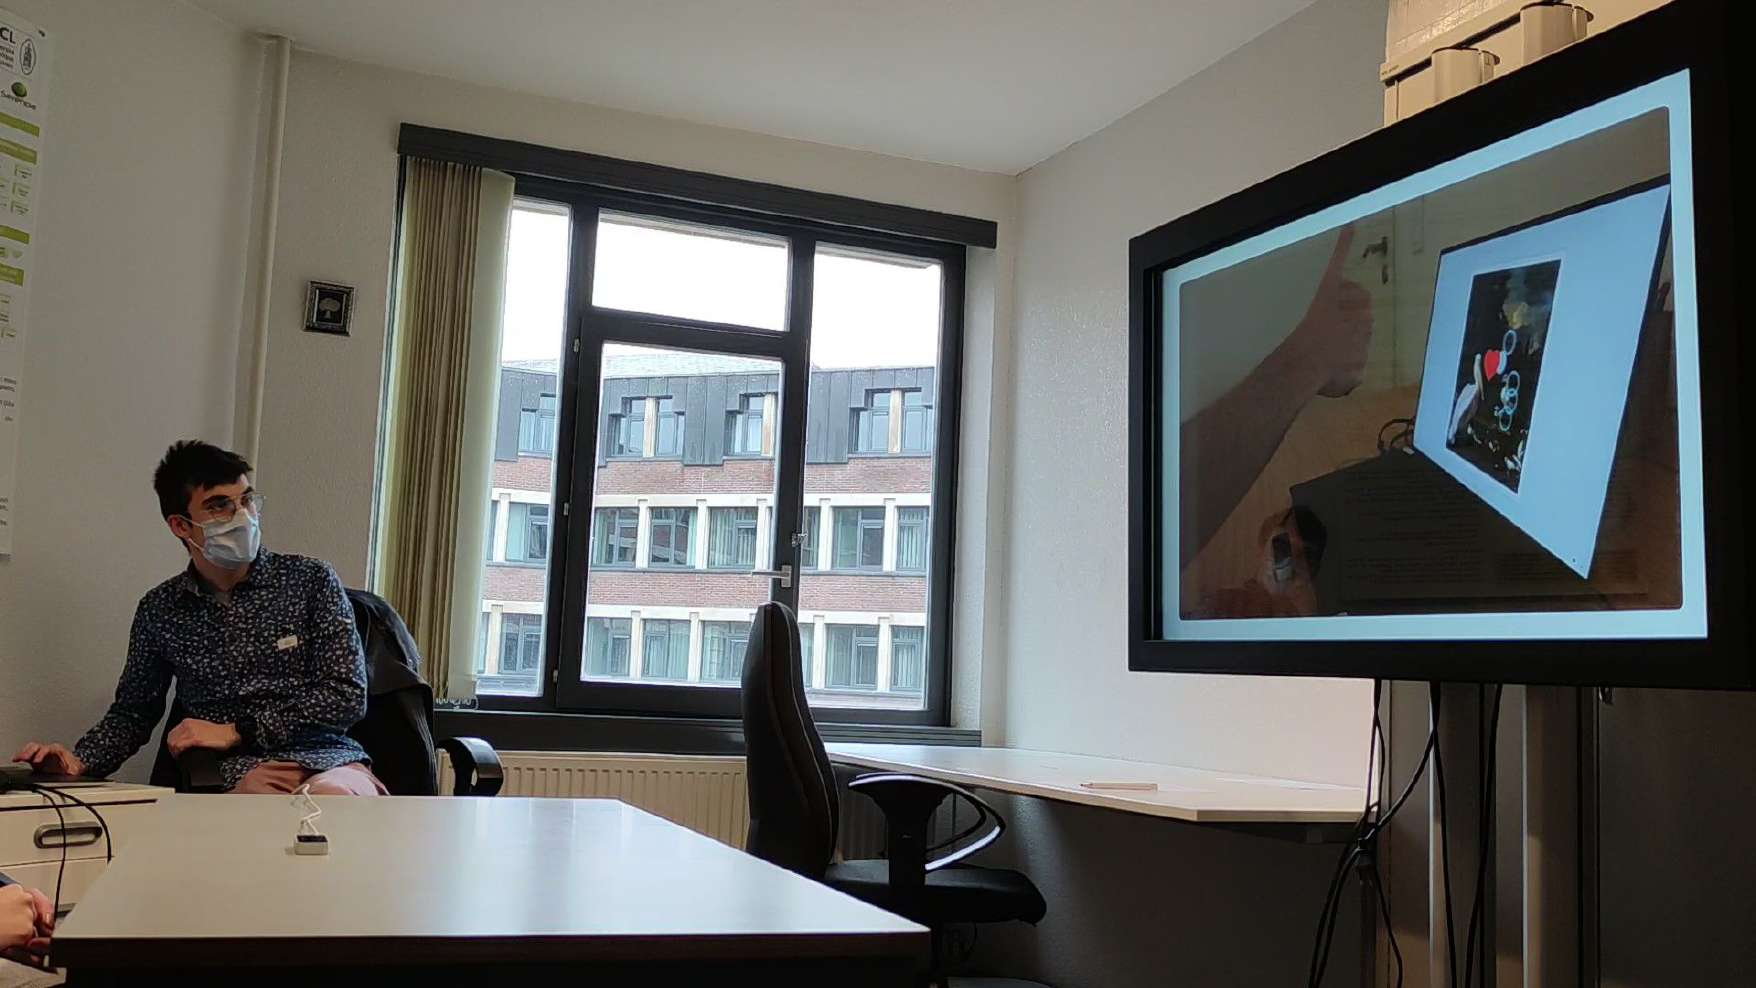
\includegraphics[width=\linewidth,trim={75 0 35 0},clip]{Figures/LUI/Evaluation/experiment-tutorial.pdf}
        \vspace{-14pt}
        \captionsetup{width=.9\linewidth}
        \caption{Tutorial video playing on the screen.}
        \label{fig:lui:evaluation-apparatus-tutorial}
    \end{subfigure}
    \begin{subfigure}{.495\textwidth}
        \centering
        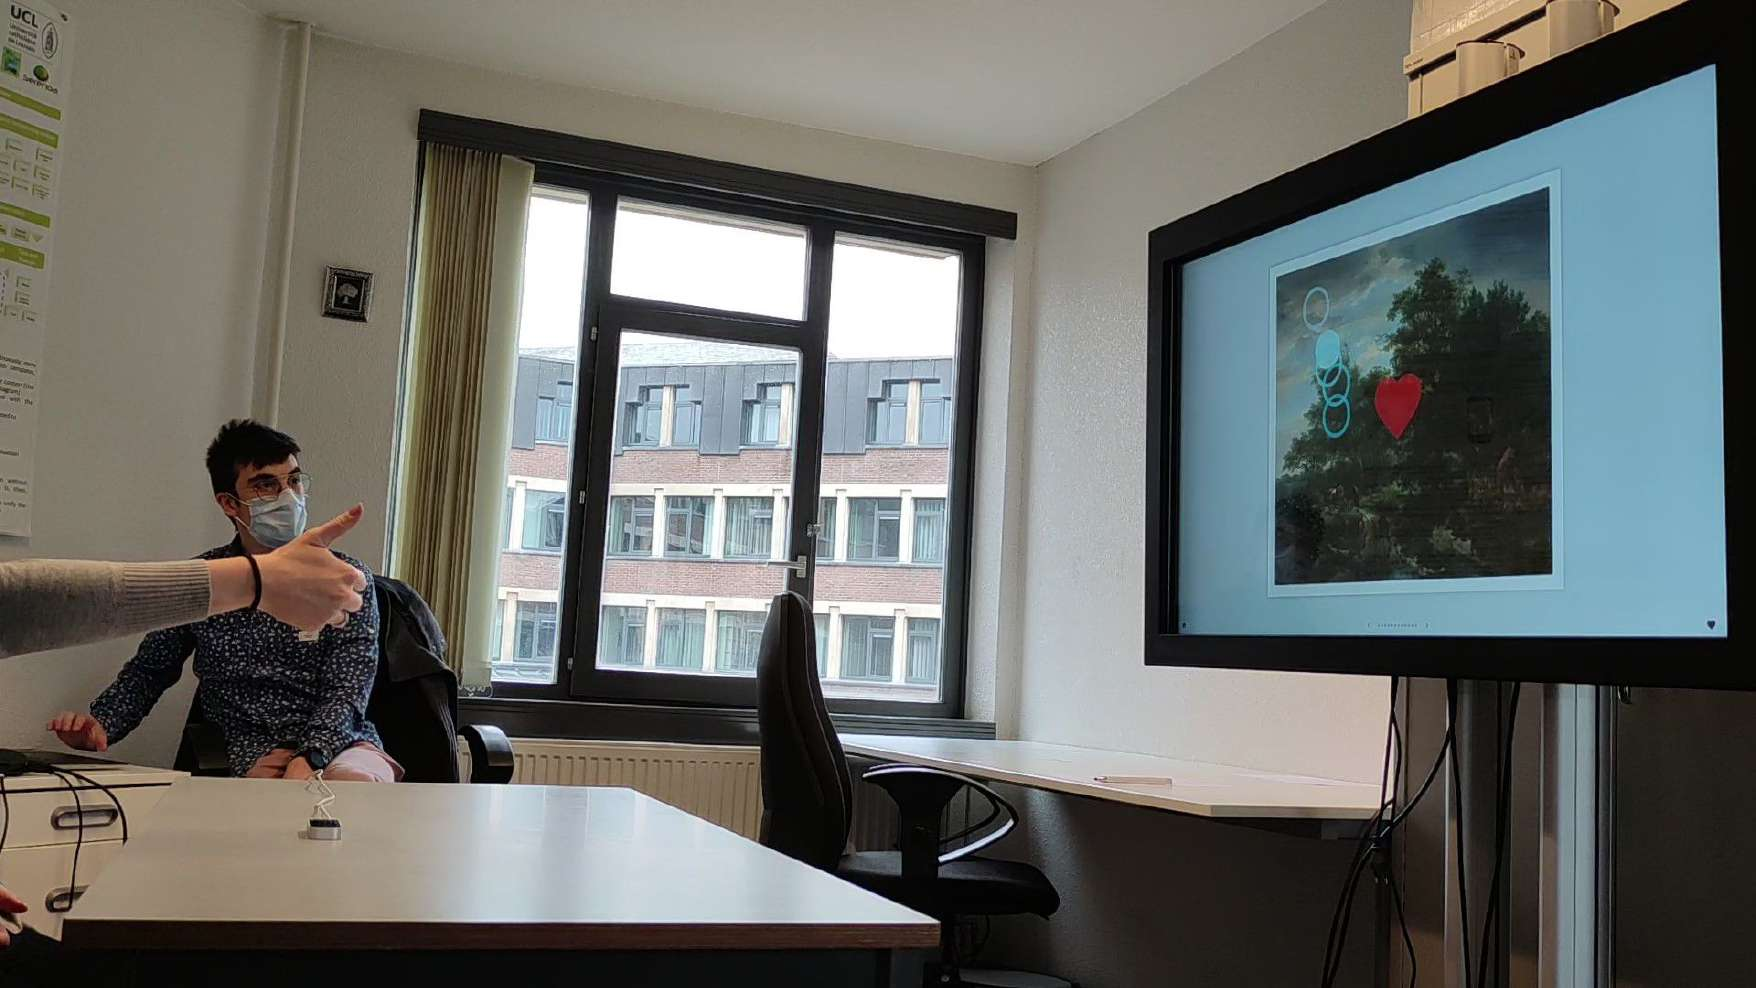
\includegraphics[width=\linewidth,trim={80 0 30 0},clip]{Figures/LUI/Evaluation/experiment-gesture.pdf} 
        \vspace{-14pt}
        \captionsetup{width=.9\linewidth}
        \caption{Participant performing a gesture.}
        \label{fig:lui:evaluation-apparatus-gesture}
    \end{subfigure}
    \vspace{-18pt}
    \caption{The setup of the experiment.}
    \label{fig:lui:evaluation-apparatus}
    % \vspace{-8pt}
\end{figure}

\subsubsection{Participants}
A stratified sampling of 17 participants (8 females and 9 males), aged between 22 and 65 years old ($M{=}37.5$, $SD{=}15.3$ years) was randomly selected from a list of volunteers to balance between genders, backgrounds, and ages (\tab~\ref{tab:lui:participants-distribution}). All participants were right-handed and all of them used smartphones daily. All but one participant ($\frac{16}{17}{=}94.1\%$) used computers at least once a week, and only two participants ($\frac{2}{17}{=}11.8\%$) frequently used gestural interaction. Occupations included student, researcher, employee, computer scientist, physiotherapist, and accountant.

\begin{table*}[tb]
    \footnotesize
    \centering
	\renewcommand{\arraystretch}{1.1}
	\captionsetup{justification=centering}
	\begin{tabular}{l>{\centering\arraybackslash}p{0.82cm}>{\centering\arraybackslash}p{0.82cm}>{\centering\arraybackslash}p{0.82cm}>{\centering\arraybackslash}p{0.82cm}>{\centering\arraybackslash}p{0.82cm}>{\centering\arraybackslash}p{0.82cm}>{\centering\arraybackslash}p{0.82cm}>{\centering\arraybackslash}p{0.82cm}}
	    \toprule
	    Gender & \multicolumn{4}{c}{\textcolor{white}{Female} \cellcolor{grayblue}} & \multicolumn{4}{c}{\textcolor{white}{Male} \cellcolor{grayblue+}} \\
	    Background & \multicolumn{2}{c}{\textcolor{white}{Technical} \cellcolor{graybluebright-}} & \multicolumn{2}{c}{\textcolor{white}{Non-technical} \cellcolor{graybluebright}} & \multicolumn{2}{c}{\textcolor{white}{Technical}\cellcolor{graybluebright-}} & \multicolumn{2}{c}{\textcolor{white}{Non-technical}\cellcolor{graybluebright}} \\
	    Age [years] & ${\leq}$ 30 \cellcolor{graybluebrighter} & ${>}$ 30 \cellcolor{graybluebrighterer} & ${\leq}$ 30  \cellcolor{graybluebrighter} & ${>}$ 30 \cellcolor{graybluebrighterer} & ${\leq}$ 30 \cellcolor{graybluebrighter} & ${>}$ 30 \cellcolor{graybluebrighterer} & ${\leq}$ 30 \cellcolor{graybluebrighter} & ${>}$ 30 \cellcolor{graybluebrighterer} \\
	    \#participants & 2 \cellcolor{graybluebrighter} & 2 \cellcolor{graybluebrighterer} & 2 \cellcolor{graybluebrighter} & 2 \cellcolor{graybluebrighterer} & 2 \cellcolor{graybluebrighter} & 2 \cellcolor{graybluebrighterer} & 2 \cellcolor{graybluebrighter} & 3 \cellcolor{graybluebrighterer} \\
        \bottomrule
	\end{tabular}
	\vspace{-4pt}
	\caption{Distribution of the participants in our study.}
	% \vspace{-10pt}
	\label{tab:lui:participants-distribution}
\end{table*}

\subsubsection{Procedure and Tasks}
The experiment consisted of two sessions conducted on separate days. The interval between the first and the second sessions of a participant ranged from 3 to 14 days ($M{=}7$, $SD{=}2.2$ days). 

\paragraph{Session 1 (Discovery and Short-term Memorability).} The first session was aimed at introducing \lui to participants and evaluating its user experience and the short-term memorability of its gesture set. It consisted of six phases:

\begin{table*}[!tb]
    \footnotesize
    \centering
    \renewcommand{\arraystretch}{1.1}
    \captionsetup{justification=centering}
    \begin{tabular}{llp{3.7cm}>{\raggedright\arraybackslash}p{3.4cm}}
        \toprule
        \textbf{Id} & \textbf{Task} & \textbf{Target(s)} & \textbf{Gestures}\\
        \midrule
        A1 & Previous & Photo, video, document, page & Flick right \\
        A2 & Next & Photo, video, document, page & Flick left \\
        A3 & Enable fullscreen & Photo, video, document, app & Tap \\
        A4 & Disable fullscreen & Photo, video, document, app & Flick up \\
        A5 & Zoom in & Photo, document, map & Pinch out \\
        A6 & Zoom out & Photo, document, map & Pinch in \\
        A7 & Volume up & Video & Swipe up \\
        A8 & Volume down & Video & Swipe down \\
        A9 & Rotate clockwise & Photo, document & Rotate a knob clockwise \\
        A10 & Rotate anti-clockwise & Photo, document & Rotate a knob anti-clockwise \\
        A11 & Play & Video & Tap \\
        A12 & Pause & Video & Tap \\
        A13 & Like & Photo & Thumbs up \\
        A14 & Dislike & Photo & Thumbs down \\
        A15 & Fast-forward & Video & Swipe left\\
        A16 & Rewind & Video & Swipe right \\
        A17 & Pan & Map & Move hand while pointing index \\
        \bottomrule
    \end{tabular}
    \vspace{-4pt}
    \caption{The 17 atomic tasks, target content, and associated gestures.}
    % \vspace{-10pt}
    \label{tab:lui:tasks-atomic}
\end{table*}

\begin{table*}[tb]
    \footnotesize
    \renewcommand{\arraystretch}{1.1}
    \captionsetup{justification=centering}
    \begin{tabular}{llp{0.5\linewidth}p{0.25\linewidth}}
        \toprule
        \textbf{Id} & \textbf{Task} & \textbf{Instructions} & \textbf{Required actions}\\
        \midrule
        C1 & Maps & In the Maps app, move and enlarge the map so that the two blue markers are situated at the left and right sides of the screen. & Enable fullscreen, zoom in, pan  \\
        C2 & Photos & In the Photos app, manipulate the windmill painting so that the author's name is the right way up and large enough to be easily readable. & Enable fullscreen, next, zoom in, rotate clockwise\slash anticlockwise \\
        C3 & Videos & In the Videos app, find the words pronounced halfway through the ``sea turtles'' video. Fast-forward through the video to get to the right part. & Enable fullscreen, next, play, fast-forward \\
        \bottomrule
    \end{tabular}
    \vspace{-4pt}
    \caption{The three compound tasks and the minimum set of actions required to complete each task.}
    % \vspace{-10pt}
    \label{tab:lui:tasks-compound}
\end{table*}

\begin{enumerate}
    \item \textit{Consent form and demographic information.} The participants were introduced to the procedure and informed that they could choose to leave the experiment at any time. They were then invited to sign a GDPR-compliant consent form and fill in a demographic survey with information such as their age, gender, level of education, occupation, digital skills~\cite{Rose:2012}, and previous experience with technologies such as smartphones, computers, and gestural interaction.
    
    \item \textit{Discovery phase.} Participants interacted freely with the \lui application for three minutes, starting from the app menu. They did not receive any specific instructions or information about the interface, except that it was controllable using the movements of the right hand above the sensor, without touching any surface. This phase served as a first introduction of \lui to the participants.
    
    \item \textit{Learning phase.} This phase served to teach the gestures to the participants and let them familiarize themselves with the system. The participants were given 17 tasks in a random order (\tab~\ref{tab:lui:tasks-atomic}). Each task was read aloud by the experimenter, who then played a short tutorial video of the associated gesture (\fig~\ref{fig:lui:evaluation-apparatus-tutorial}). 
    The use of videos ensured that all participants received the same instructions. Once the tutorial finished playing, the experimenter loaded the associated page of the \lui application and prompted the participants to perform the gesture in order to complete the task (\fig~\ref{fig:lui:evaluation-apparatus-gesture}). Participants could re-watch the tutorial videos as many times as necessary. If a participant accidentally left the current page (\eg by performing the wrong gesture), the experimenter informed them and re-loaded the correct page.  %The task was skipped after four failed attempts.
    
    \item \textit{Resting phase.} Participants were given five minutes to rest in a separate room.
    
    \item \textit{Testing phase.} This phase aimed to evaluate the short-term memorability of the gesture set by asking participants to perform 20 tasks with no external help. The participants first completed 17 atomic tasks (\tab~\ref{tab:lui:tasks-atomic}) in a random order, following a similar procedure to the learning phase: the experimenter first read the task aloud, loaded the associated page of the \lui application, and prompted the participants to perform the gesture. The target content was randomly selected for each task (\eg for the ``zoom in'' task, the target could be a picture, a document, or a map) and the tasks were grouped by target content.
    The participants then performed three compound tasks (\tab~\ref{tab:lui:tasks-compound}). For each compound task, the experimenter read the task aloud, loaded the application menu, and prompted the participants to perform the task. Participants could request the experimenter to repeat the instructions or to go back to the application menu.

    Participants were instructed to fill in at the end of each session a UEQ+ questionnaire (User Experience Questionnaire)~\cite{Schrepp:2017}, a modular extension of UEQ in which we selected 7 scales (\ie attractiveness, efficiency, perspicuity, dependability, stimulation, usefulness, and intuitive use) among 20 scales to focus on evaluating the user experience of participants interacting by gestures with \lui. Each scale is, in turn, decomposed into four subscales to be evaluated (\eg attractiveness is decomposed into four subscales: annoying \vs enjoyable, bad \vs good, unpleasant \vs pleasant, and unfriendly \vs friendly), each subscale being a differential scale with 7 points between items of each pair (\eg annoying o o o o o o o enjoyable). 

    \item \textit{Questionnaire.} Participants were asked to complete a UEQ+ questionnaire (User Experience Questionnaire)~\cite{Schrepp:2017}, a modular extension of UEQ. We selected 7 UEQ+ scales (\ie attractiveness, efficiency, perspicuity, dependability, stimulation, usefulness, and intuitive use) among the 20 available scales to focus on evaluating the user experience of participants interacting by gestures with \lui. Each scale consists of four subscales to be evaluated (\eg attractiveness is decomposed into four subscales: annoying \vs enjoyable, bad \vs good, unpleasant \vs pleasant, and unfriendly \vs friendly).
    %\item \textit{Interview and questionnaires.} After completing the testing phase, participants were interviewed to collect their feedback about the \lui application. The interview consisted of three questions: (1) ``What is the first positive thing that comes to mind regarding your experience with the \lui application?'', (2) ``What is the first negative thing that comes to mind regarding your experience with the \lui application?'', and (3)``Do you have any other comments?''. Then, they were asked to complete a questionnaire consisting of seven UEQ+ scales.
    % and three ad hoc scales targeting the discoverability, learnability, and social acceptability of the \lui application.
\end{enumerate}

\paragraph{Session 2 (Long-term Memorability).} The second session was much shorter and consisted of only three phases:
\begin{enumerate}
    \item \textit{Introduction.} Participants were welcomed and reminded of the procedure, in particular, that they could leave the experiment at any time.
    
    \item \textit{Testing phase.} This second testing phase served to evaluate the long-term memorability of the \lui gesture set. We followed the same procedure as in the testing phase of the first session.
    
    \item \textit{Questionnaire.} At the end of the session, participants were asked to fill in the same UEQ+ questionnaire as in the first session.
\end{enumerate}

\subsubsection{Metrics and Data Collection}
We collected a set of metrics for the learning and testing phases of both sessions to give us insight into the performance and usability of the system:
\begin{enumerate}
    \item The \custominlinehighlight{Task Success Rate} measures the percentage between the number of successful tasks (\ie the gesture is correctly remembered, produced, and recognized) and the total number of executed tasks. An atomic task was considered successful if it was correctly executed within a maximum of four trials. Regarding compound tasks, the number of trials was not limited since they required participants to perform several gestures in an undefined order. We thus considered a compound task unsuccessful only if it was skipped by the participant.
    \item The \custominlinehighlight{Number of Trials} measures the total number of gestures executed for each task, whether successful, incorrectly recalled, incorrectly executed, or incorrectly recognized by the system.
    % \item The \custominlinehighlight{Thinking-time} measures the time, in seconds, needed by participants to remember a gesture for a given task.
    % \item The \custominlinehighlight{Memorability rate} measures the percentage between the number of correctly remembered gestures and the total number of gestures produced.
    % \item The \custominlinehighlight{Recognition rate} measures the percentage between the number of correctly recognized gestures and the total number of gestures produced. Note that a gesture could be properly remembered by a participant, but not accurately recognized by \lui or could be inadequately remembered, but accurately recognized. In the first case, it is \lui's fault. In the second case, it is the participant's fault.
\end{enumerate}
%Each scale consists of 4 pairs of items with opposite meanings with a 7-point Likert scale + 1 item for estimating the relevance of the scale. 
% (2) three ad hoc scales to assess the perceived discoverability, learnability, and social acceptability of the \lui gestural interface. The discoverability scale was removed from the questionnaire of the second session of the experiment as it was no longer relevant.
In addition to the metrics, demographic information, and questionnaires, we captured video footage of the discovery, learning, and testing phases.

\begin{table*}[!hbt]
    \renewcommand{\arraystretch}{1.1}
    \footnotesize
    \centering
    \begin{tabular}{lp{3.45cm}ccc}
        \toprule
        \textbf{Id} & \textbf{Task} & \textbf{Learning phase} & \textbf{Testing phase 1} & \textbf{Testing phase 2} \\
        \midrule
        A1 & Previous & 100\% & 100\% & 100\%  \\ 
        A2 & Next & 100\% & 94\% & 94\%  \\ 
        A3 & Enable fullscreen & 88\% & 82\% & 100\%  \\ 
        A4 & Disable fullscreen & 76\% & 88\% & 100\%  \\ 
        A5 & Zoom in & 100\% & 88\% & 94\%  \\ 
        A6 & Zoom out & 94\% & 94\% & 82\%  \\ 
        A7 & Volume up & 94\% & 88\% & 82\%  \\ 
        A8 & Volume down & 82\% & 100\% & 94\%  \\ 
        A9 & Rotate clockwise & 71\% & 71\% & 71\%  \\ 
        A10 & Rotate anti-clockwise & 82\% & 82\% & 71\%  \\ 
        A11 & Play & 82\% & 88\% & 100\%  \\ 
        A12 & Pause & 94\% & 88\% & 82\%  \\ 
        A13 & Like & 100\% & 100\% & 100\%  \\ 
        A14 & Dislike & 100\% & 100\% & 94\%  \\ 
        A15 & Fast-forward & 88\% & 88\% & 88\%  \\ 
        A16 & Rewind & 82\% & 82\% & 71\%  \\ 
        A17 & Pan & 88\% & 88\% & 88\%  \\ 
        \midrule
        C1 & Photo & -- & 100\% & 94\%  \\ 
        C2 & Video & -- & 82\% & 94\%  \\ 
        C3 & Map & -- & 76\% & 65\% \\ 
        \bottomrule
    \end{tabular}
    \vspace{-4pt}
    \caption{Success rate for the 17 atomic and 3 compound tasks.}
	% \vspace{-10pt}
	\label{tab:lui:success-rate}
\end{table*}

%--------------------------------------------------------------------------------%
\subsection{Results and Discussion} \label{sec:lui:evaluation:results}
\subsubsection{Task Success Rate}
\tab~\ref{tab:lui:success-rate} gives the success rate for the atomic and compound tasks.
Only two atomic tasks have a success rate below 80\% in the learning phase: tasks A4 (disable full screen) and A9 (rotate clockwise). In the first testing phase, only task A9 has a success rate below 80\%, while in the second testing phase, the overall success rate decreases slightly, and three tasks have a success rate lower than 80\%: tasks A9, A10 (rotate anticlockwise), and A16 (rewind). 
Overall, the lower success rate of the rotating (anti-)clockwise tasks may be explained by the high sensitivity of the system to the users' hand pose. For instance, if the users' fingers were too far apart when performing the ``grab'' gesture, it was not recognized by the system. To a lesser extent, this high sensitivity may have affected the recognition of other static gestures (see \tab~\ref{tab:lui:elicitation-to-recognition}), such as in the ``fast-forward'', ``rewind'', and ``pan'' tasks.

\begin{table*}[!b]
    \renewcommand{\arraystretch}{1.1}
    \footnotesize
    \centering
    \begin{tabular}{lp{3.1cm}cccccc}
        \toprule
        \multirow{2}{*}{\textbf{Id}} & \multirow{2}{*}{\textbf{Task}} & \multicolumn{2}{c}{\textbf{Learning phase}} & \multicolumn{2}{c}{\textbf{Testing phase 1}} & \multicolumn{2}{c}{\textbf{Testing phase 2}} \\
        ~ & ~ & Mean & Median & Mean & Median & Mean & Median \\
        \midrule
        A1 & Previous & 1,2 & 1 & 1,6 & 1 & 1,7 & 1  \\
        A2 & Next & 1,1 & 1 & 1,3 & 1 & 1,6 & \cellcolor{highlightcolor}2  \\
        A3 & Enable fullscreen & 1,5 & 1 & 1,5 & 1 & 1,1 & 1  \\
        A4 & Disable fullscreen & 1,2 & 1 & 1,7 & \cellcolor{highlightcolor}2 & 1,5 & 1  \\
        A5 & Zoom in & 1,4 & 1 & 1,3 & 1 & 1,5 & 1  \\
        A6 & Zoom out & 1,4 & 1 & 1,1 & 1 & 1,2 & 1  \\
        A7 & Volume up & 1,3 & 1 & 1,3 & 1 & 1,1 & 1  \\
        A8 & Volume down & 2,0 & \cellcolor{highlightcolor}2 & 1,5 & 1 & 1,3 & 1  \\
        A9 & Rotate clockwise & 2,1 & \cellcolor{highlightcolor}1,5 & 1,6 & \cellcolor{highlightcolor}1,5 & 1,9 & \cellcolor{highlightcolor}1,5  \\
        A10 & Rotate anti-clockwise & 1,8 & \cellcolor{highlightcolor}1,5 & 2,1 & \cellcolor{highlightcolor}1,5 & 2,4 & \cellcolor{highlightcolor}2,5  \\
        A11 & Play & 1,3 & 1 & 2,0 & 1 & 1,6 & 1  \\
        A12 & Pause & 1,4 & 1 & 1,5 & 1 & 1,8 & \cellcolor{highlightcolor}1,5  \\
        A13 & Like & 1,0 & 1 & 1,2 & 1 & 1,3 & 1  \\
        A14 & Dislike & 1,0 & 1 & 1,1 & 1 & 1,0 & 1  \\
        A15 & Fast-forward & 1,7 & 1 & 1,7 & 1 & 1,9 & \cellcolor{highlightcolor}2  \\
        A16 & Rewind & 1,4 & 1 & 1,7 & 1 & 1,4 & 1  \\
        A17 & Pan & 1,3 & 1 & 1,3 & 1 & 1,5 & 1 \\
        \bottomrule
    \end{tabular}
    \vspace{-4pt}
    \captionsetup{width=.99\linewidth}
    \caption{Number of trials for successful completion of each atomic task.}
	\vspace{-10pt}
	\label{tab:lui:trials}
\end{table*}


Regarding compound tasks, tasks C1 (photo) and C2 (video) had a higher success rate than task C3 (map) in both the first and second testing phases. The ``pan'' gesture used in the Maps application was not elicited, which may have impacted the usability of the application. In addition, this task required more precision than the other two, as it required participants to accurately manipulate the map so that two markers were situated on each side of the screen.

\begin{figure}[!b]
    \centering
    \begin{subfigure}{.495\linewidth}
        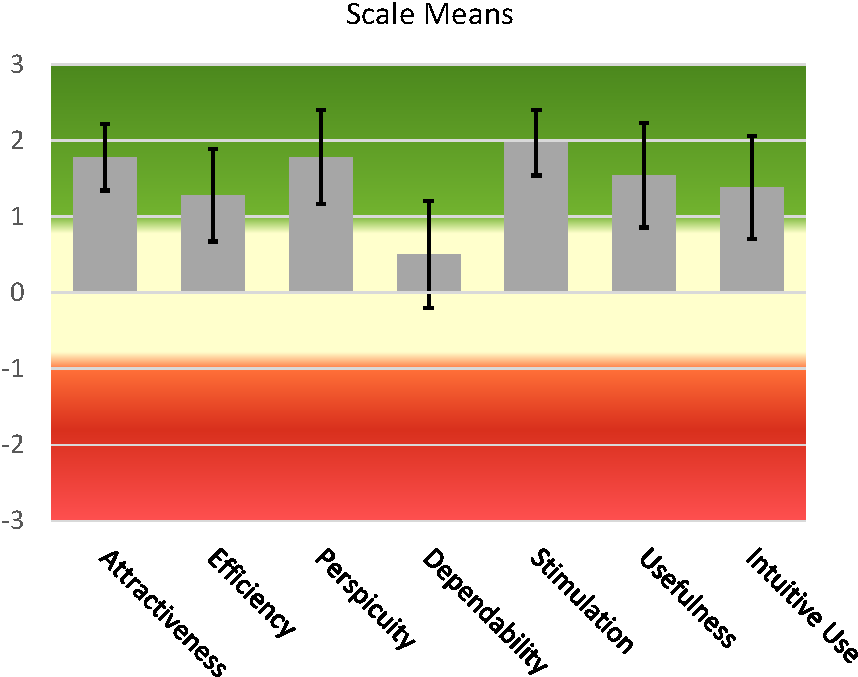
\includegraphics[width=\linewidth]{Figures/LUI/Evaluation/ueq+_session_1_scale_means.pdf}
        \caption{Session 1.}
        \label{fig:lui:ueqplus-scales:session1}
    \end{subfigure}
    \begin{subfigure}{.495\linewidth}
        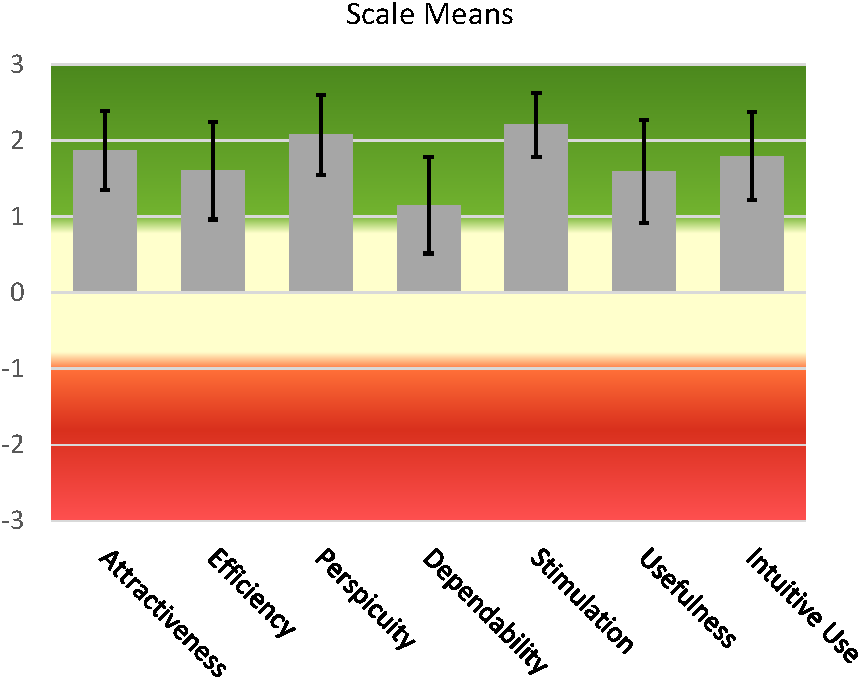
\includegraphics[width=\linewidth]{Figures/LUI/Evaluation/ueq+_session_2_scale_means.pdf}
        \caption{Session 2.}
        \label{fig:lui:ueqplus-scales:session2}
    \end{subfigure}
    \vspace{-16pt}
    \caption{Mean score for each scale of the UEQ+ questionnaire.}
    \label{fig:lui:ueqplus-scales}
    % \vspace{-8pt}
\end{figure}

\subsubsection{Number of Trials}

\tab~\ref{tab:lui:trials} gives the average and median number of tries needed to successfully complete the atomic tasks. These metrics are presented for the learning session and the two testing sessions, allowing in particular to study the memorability of gestures.

As presented, most tasks were completed with a single try. The most problematic tasks were the rotations, whether clockwise or anticlockwise. We can also observe that more attempts were needed to pass the tasks in session 2, especially for A1 (previous), A2 (next), A12 (pause), and A15 (fast forward). On the contrary, the tasks of increasing or decreasing the volume (A7 and A8) required fewer tries over time.

\subsubsection{Results of the UEQ+ Questionnaire}
Users' answers to the 7 selected UEQ+ scales were computed and interpreted
with the \href{https://ueqplus.ueq-research.org/Material/UEQ_Plus_Data_Analysis_Tool.xlsx}{UEQ data analysis tool}. \fig~\ref{fig:lui:ueqplus-scales} represents the mean score for each selected scale on an interval [-3,...,+3], where a value of -3 expresses the weakest value and +3 expresses the strongest value for both sessions (first in \fig~\ref{fig:lui:ueqplus-scales:session1} and second in \fig~\ref{fig:lui:ueqplus-scales:session2}).
If we stick to the interpretation that a value greater than or equal to 0.8 represents a positive evaluation~\cite{Schrepp:2017}, then all mean scores for session 1 are considered positive (ranging from $M{=}1.28$ for efficiency to $M{=}1.97$ for stimulation), except dependability ($M{=}0.50$, $SD{=}2.22$) considered as a neutral value. This low value can be explained by the cognitive destabilization of participants producing these kinds of gestures for the first time, and being puzzled by them. However, this phenomenon was observed transiently insofar as the gestures, initially felt to be difficult to produce because they were unknown, then became easier to produce. Indeed, dependability increased by 130\% ($M{=}1.15$, $SD{=}1.80$) in session 2. 
Mean scores for session 2 are all superior to those obtained for session 1 and range from 
$M{=}1.15$ for dependability to $M{=}2.21$ for stimulation. The mean score for some scales even largely increased, such as efficiency (from $M{=}1.28$ to $M{=}1.60$), perspicuity (from $M{=}1.78$ to $M{=}2.07$), and intuitive use (from $M{=}1.38$ to $M{=}1.79)$.
The KPI (Key Performance Indicator) computed by UEQ+~\cite{Hinderks:2019} increased from 1.44 for session 1 to 1.74 for session 2, confirming the overall positive evolution.

%================================================================================%
\section{Discussion} \label{sec:lui:discussion}
In this section, we discuss the main strengths and limitations of the \lui application, which we designed following a user-centered iterative development method.
%--------------------------------------------------------------------------------%
\subsection{Strengths} \label{sec:lui:discussion:strengths}
The main strengths of \lui lie in the three requirements defined in Section~\ref{sec:lui:description:requirements}, which we now revisit in the light of this work:
%
\begin{enumerate}
    \item \textit{Consistency.} The gesture set of \lui was designed to be consistent across the various types of media contents, by assigning similar gestures to similar functions, regardless of the media type. In addition, it is expected to be compliant with end users' expectations as the gesture set was based on a contextual gesture elicitation study.
    \item \textit{Continuity.} The \lui application supports continuous interaction with media contents thanks to \ql. The segmentation module allows the continuous recognition of gestures while they are being issued, without input from the user, and the static recognizer enables the manipulation of media objects with immediate and continuous feedback.
    \item \textit{Customizability.} Thanks to \ql, the \lui application supports customizability by enabling users with no coding skills to include their own gestures in three steps (\fig~\ref{fig:lui:customization-steps}): (1) record new gesture samples using custom software, \eg our LeapGesturePlayback tool\footnote{The code of the gesture recording tool is available on GitHub at \url{https://github.com/sluyters/LeapGesturePlayback}.} (\fig~\ref{fig:lui:customization-steps:record}), (2) overwrite the old gesture files with the new samples (\fig~\ref{fig:lui:customization-steps:files}), and (3) restart \ql to propagate the changes, which takes less than ten seconds on a modern computer.
\end{enumerate}

\begin{figure}[p]
    \centering
    
    \begin{subfigure}{.90\textwidth}
        \centering
        \fbox{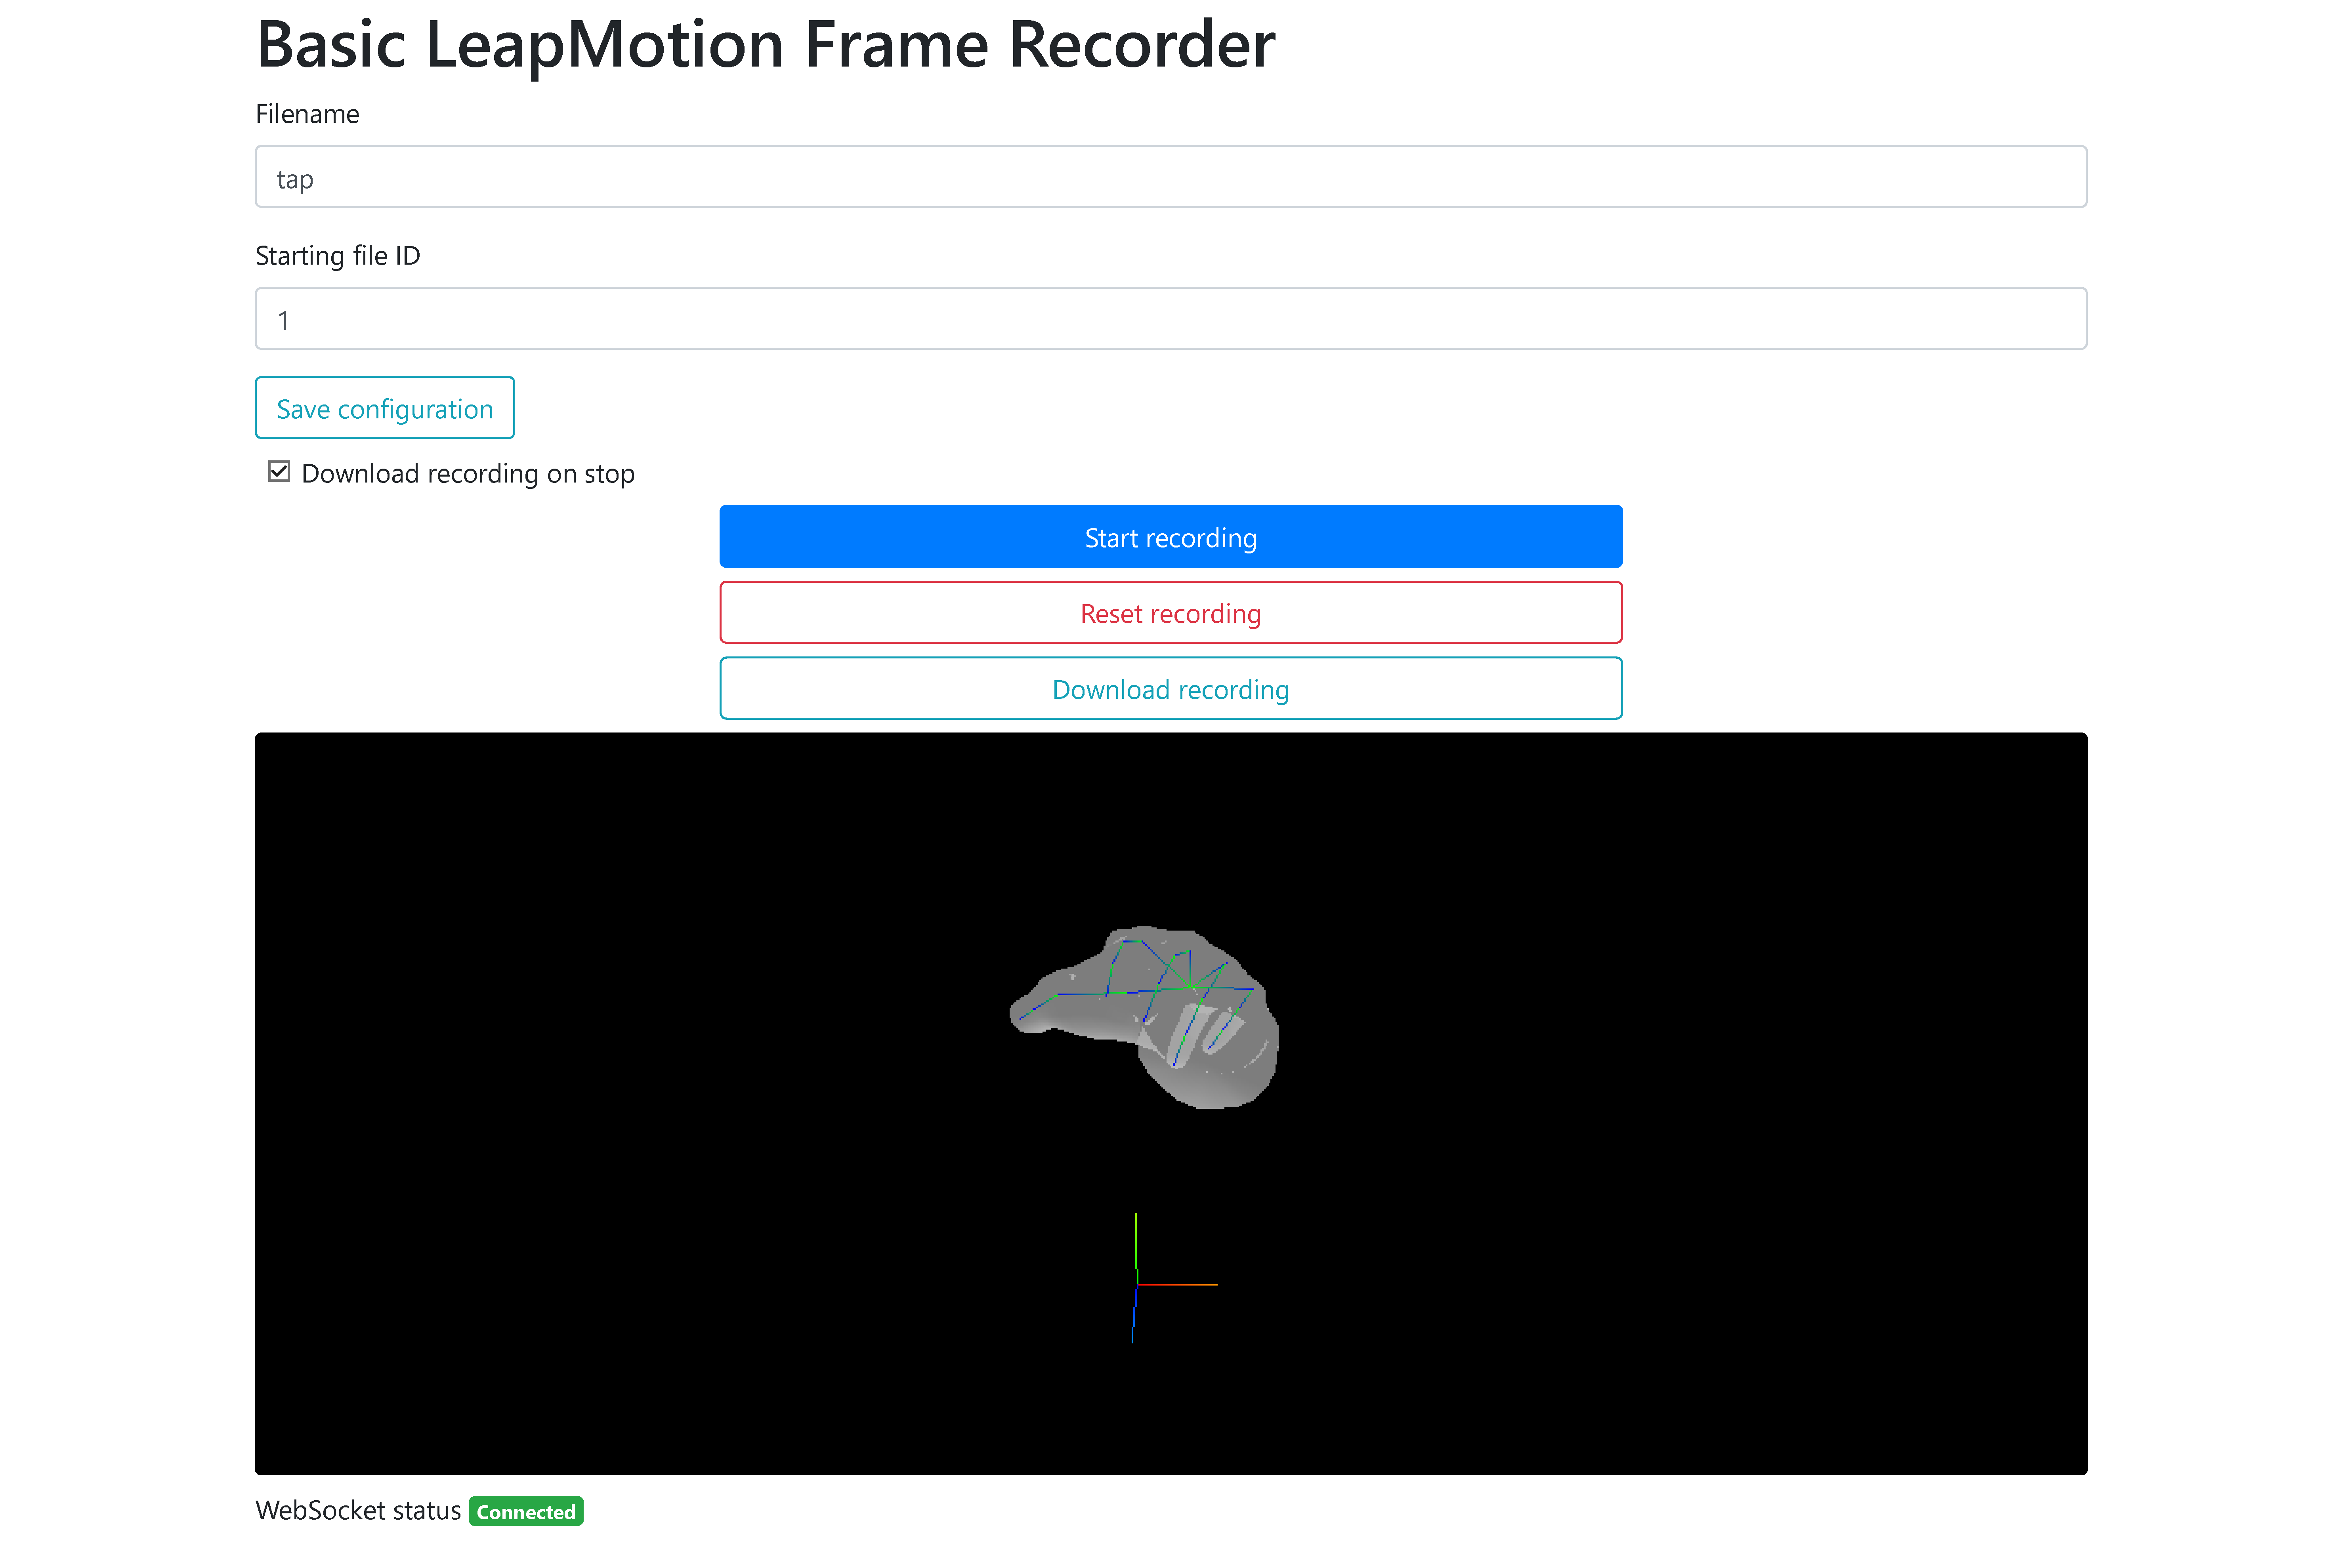
\includegraphics[width=.97\linewidth]{Figures/LUI/Customization/recorder.pdf}} 
        \captionsetup{width=.99\linewidth}
        \vspace{-2pt}
        \caption{Recording new gesture samples.}
        \label{fig:lui:customization-steps:record}
    \end{subfigure}
    \vspace{2pt}
    
    \begin{subfigure}{.90\textwidth}
        \centering
        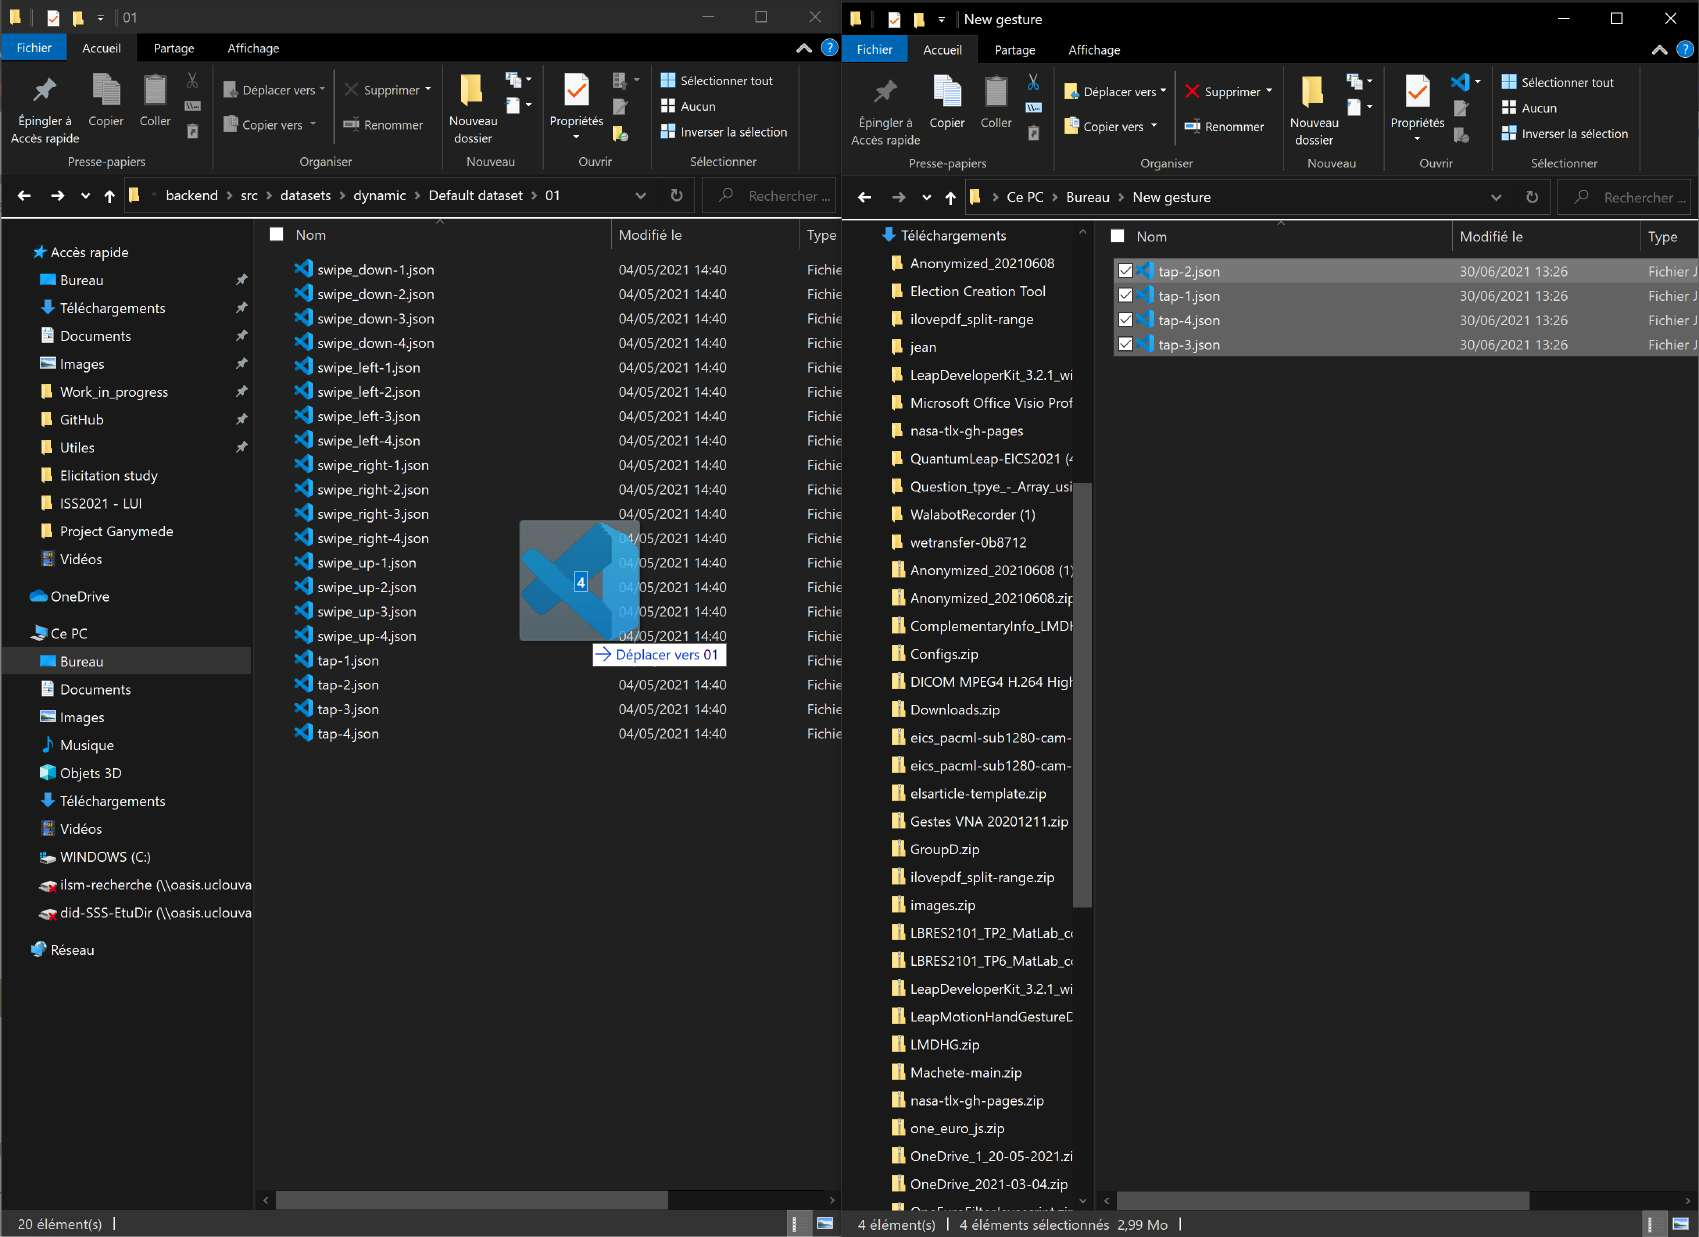
\includegraphics[width=.99\linewidth]{Figures/LUI/Customization/files.pdf}  
        \vspace{-2pt}
        \captionsetup{width=.99\linewidth}
        \caption{Replacing old gesture files with new samples.}
        \label{fig:lui:customization-steps:files}
    \end{subfigure}
    \vspace{-6pt}
    \caption{Two main steps for customizing the \lui gesture set.}
    \label{fig:lui:customization-steps}
    % \vspace{-16pt}
\end{figure}

%--------------------------------------------------------------------------------%
\subsection{Limitations} \label{sec:lui:discussion:limitations}
The \lui application has a few limitations, some of which arise from its use of the \ql framework.
%
First, while utilizing simple template-matching recognizers allows users to quickly and easily customize the \lui gesture set with their own gestures, employing properly trained state-of-the-art machine learning recognizers might accommodate a broader range of gestures and enable better gesture recognition accuracy. 
% Gesture set modifications
Moreover, taking into account modifications to the gesture set requires a restart of \ql. Although this process is swift thanks to the use of template-matching recognizers~\cite{Brunelli:2009}, as opposed to neural network-based recognizers which may require extensive re-training before recognizing the updated gesture set~\cite{Brunelli:2009}, the need for a restart could be avoided altogether. 
%
In addition, the customization process could be further streamlined and simplified by integrating it into the \lui application, enabling users to modify the gesture set without leaving the application.
% Segmentation
Furthermore, gesture segmentation is not perfect, and parasitic motion may be mistaken for a gesture intended by the user, despite the workarounds that we implemented (\eg rejection thresholds). Hence, users must remain careful while interacting with the application to avoid triggering actions inadvertently.
% Multi-user
Lastly, \lui does not support concurrent interaction from multiple users due to limitations of \ql. As a result, concurrent gestures from two users will interfere with each other.

Other limitations of \lui are related to our development method, specifically, the design of the gesture set and the proposed evaluation procedure.
%
First, user fatigue may become a problem during long interactions with \lui, as mid-air gestures can be more tiring than traditional interaction methods~\cite{Siddhpuria:2017,Jakobsen:2015,Hansberger:2017} (Section~\ref{sec:state_of_the_art:overview:challenges:gorilla-arm}). Minimizing the physical effort of mid-air gestures is critical to supporting prolonged gesture interaction~\cite{Hansberger:2017}.
%
Then, while user-elicited gesture sets have been shown to improve the immediate usability of an application~\cite{Wobbrock:2005}, the GES procedure followed in this chapter is not without flaws.
Indeed, the small sample size of our study may also not accurately represent the majority of the population, as gesture propositions are affected by participants' cultural background~\cite{Archer:1997}. 
Our choice of illustrations for the referents featured notable differences from the final LUI application and may have influenced participants' gesture propositions. 
In addition, GESs usually rely on subjective criteria for gesture clustering, which may further impact the validity of their findings~\cite{Vatavu:2019}. 
Fortunately, the customizability of \lui contributes to mitigating these issues by enabling end users to define their own set of gestures.
%
Finally, our evaluation procedure focused on collecting quantitative data. While this approach is a great way to evaluate the usability of an application, it provides little insight into the actual reasons behind user challenges and potential avenues for improvement. Collecting additional qualitative data, \eg by incorporating thinking-aloud techniques~\cite{vanSomeren:1994} into our evaluation procedure, would provide us with a more comprehensive understanding of users' thoughts and reasoning.


%================================================================================%
\section{Conclusion} \label{sec:lui:conclusion}
% Summary
In this chapter, we introduced an iterative and participatory process for designing gesture-based applications, comprising three stages: (1) designing an intuitive and consistent gesture set based on user preferences identified from the literature or through a GES, (2) implementing a gesture recognition dataflow and identifying the most optimal algorithms for gesture recognition, and (3) evaluating the final gestural interface with potential end users of the system.
%
We applied this process in the development of \lui, a gesture-based application designed for browsing and manipulating multimedia content (images, videos, documents, and maps) on large displays. The use of the \ql framework (Chapter~\ref{chap:quantumleap}) and its testing tool (Chapter~\ref{chap:quantumleap-testing}) greatly facilitated the implementation of consistent, continuous, and customizable mid-air gesture interaction into \lui.
%
After evaluating \lui in an experiment with 17 participants, we noted an increase in its perceived usability between the two experimental sessions, despite a few participants having trouble remembering some of the gestures. We also observed some unpredictability in gesture recognition for certain gestures, attributed in part to slight variations in the way they were performed by the participants. This underscores the importance of supporting gesture set customization.

% Software quality properties
The \lui application inherits multiple ISO/IEC 25010 software quality properties~\cite{iso25010} from its use of \ql and its testing tool (Chapters~\ref{chap:quantumleap} and~\ref{chap:quantumleap-testing}), including \textit{maintainability} and \textit{portability}.
%
Our methodology also supports the \textit{usability} property, by encouraging developers to involve end users in the development process of their application, by conducting GESs to identify user preferences, and by evaluating their application among potential users.

% Future works
This chapter opens up promising avenues for future work.
% 
First, the current iteration of \lui relies exclusively on single-handed gestures, which aligns with user preferences observed in our GES. However, because these preferences may change depending on the sensor and context of use, it would be relevant to implement and evaluate the performance of the system on a gesture set of two-handed, or even whole-body gestures.
% 
In addition, we focused on a single-user scenario where one person controls the system and others are spectators. Future work could investigate multiuser scenarios of two types: (1) a collaborative scenario, where multiple users cooperate on the same screen simultaneously, and (2) a ``talking stick'' scenario where control can switch between users (\eg in a classroom or an office meeting). Implementing these scenarios might involve one device capable of sensing multiple users concurrently (\eg MS Kinect) or multiple devices, each capturing gestures from one or more users (\eg one LMC in front of each seat at a conference table).
%
Next, we could look into incorporating speech recognition into \lui, to complement mid-air gestures by providing a simple way to execute complex commands, such as searching for specific content by keywords. 
% 
Finally, if we seek to deploy the system on public displays, several challenges will certainly arise, including dealing with users' privacy concerns and a less forgiving environment. 
As such, we could investigate other types of sensors, such as radars, that address most privacy issues related to vision-based sensors and are less sensitive to environmental conditions. UI elements would also have to be carefully designed to attract users, retain their attention, and effectively communicate the supported gestures.

